% =====================================================================
%  Anatomía de un LLM — Fase VI — Módulo 27
%  Optimización geométrica y software 3D
%  Compilar: latexmk -r ../latexmkrc M27-geometria-3d.tex
% =====================================================================
\documentclass[11pt,a4paper,twoside,openany]{book}
\usepackage{../estilo-apuntes}

\newcommand{\ApuntesCurso}{Anatomía de un LLM}
\newcommand{\ApuntesModulo}{Módulo 27}

% Notación propia del módulo
\newcommand{\xf}{\tilde{x}}
\newcommand{\Emin}{E_{\min}}
\newcommand{\rmin}{r_{\min}}
\newcommand{\Vol}{\operatorname{Vol}}
\newcommand{\IoU}{\operatorname{IoU}}
\newcommand{\sigm}{\operatorname{sig}}
\newcommand{\clip}{\operatorname{clip}}
\newcommand{\diag}{\operatorname{diag}}
\newcommand{\CD}{\operatorname{CD}}
\newcommand{\T}{\top}
\newcommand{\hx}{\hat{x}}
\makeatletter\g@addto@macro\UrlBreaks{\do\-\do\/}\makeatother

\hypersetup{pdftitle={Módulo 27. Optimización geométrica y software 3D},pdfauthor={Anatomía de un LLM}}

\begin{document}
\frontmatter
% ------------------------------------------------------------------ Portada
\begin{titlepage}
\centering
\vspace*{2.5cm}
{\large\scshape Anatomía de un LLM}\par
\vspace{0.4cm}
{\normalsize Fundamentos matemáticos de los modelos de lenguaje}\par
\vspace{2.2cm}
\rule{\textwidth}{0.8pt}\par\vspace{0.5cm}
{\small\scshape Fase VI \textperiodcentered\ Diseño y construcción de optimizadores con IA}\par\vspace{0.3cm}
{\Huge\bfseries Módulo 27\par}\vspace{0.3cm}
{\LARGE Optimización geométrica y software 3D\par}
\vspace{0.2cm}
{\large Representaciones diferenciables, topología, simuladores, renderizado y pipelines 3D\par}
\vspace{0.5cm}\rule{\textwidth}{0.4pt}\par
\vspace{1.6cm}
{\large Apuntes del curso}\par
\vfill
{\small Edición de octubre de 2026}\par
\end{titlepage}

% ------------------------------------------------------- Presentación
\chapter*{Presentación del módulo}
\addcontentsline{toc}{chapter}{Presentación del módulo}
\markboth{Presentación del módulo}{}

Un optimizador geométrico busca una forma: la distribución de material de una pieza, el perfil de una aleta, la malla de un objeto reconstruido a partir de fotografías o el nivel de detalle con que se dibuja una escena. En todos los casos aparece la misma cadena: unos parámetros generan una geometría, un simulador o un renderizador la evalúan, una pérdida resume el resultado y un gradiente, calculado con el método adjunto o con diferenciación automática, indica cómo modificar los parámetros. Este módulo estudia los eslabones de esa cadena y los ensambla en casos completos. Empieza por las representaciones 3D y su diferenciabilidad; sigue con la optimización de topología por el método SIMP, que es el ejemplo clásico de diseño guiado por sensibilidades adjuntas; continúa con los simuladores diferenciables y los modelos sustitutos neuronales, y con el renderizado diferenciable, que convierte la reconstrucción 3D (incluidos NeRF y el \emph{Gaussian splatting}) en un problema de descenso de gradiente. Los dos últimos temas pasan del laboratorio a la producción: la optimización de los pipelines de software 3D y videojuegos (simplificación de mallas, niveles de detalle, compresión de texturas, empaquetado UV, automatización con Blender y presupuestos de milisegundos), y la validación de la geometría producida por modelos generativos antes de fabricarla o cargarla en un motor. Sobre productos comerciales (Autodesk Fusion, nTop, Unreal Engine) solo se usa información pública, que se cita.

\section*{Objetivos}
Al finalizar el módulo, el estudiante debe ser capaz de:
\begin{enumerate}[label=\arabic*.]
  \item describir mallas, nubes de puntos, vóxeles, funciones de distancia con signo y campos neuronales, decidir cuál conviene a un problema y calcular derivadas de magnitudes geométricas respecto a sus parámetros;
  \item formular el problema de flexibilidad mínima con la interpolación SIMP, deducir sus sensibilidades por el método adjunto, justificar los filtros y la actualización por criterios de optimalidad, e implementar el caso de la viga MBB;
  \item derivar a través de un simulador mediante el teorema de la función implícita, construir y validar un modelo sustituto y acotar el error que comete al optimizar sobre él;
  \item explicar por qué la rasterización clásica no es diferenciable, cómo la suavizan los renderizadores diferenciables y cómo NeRF y el \emph{Gaussian splatting} se entrenan por descenso de gradiente;
  \item plantear como problemas de optimización la simplificación de mallas por error cuádrico, la selección de niveles de detalle con un presupuesto de tiempo por fotograma, la compresión de texturas y el empaquetado UV;
  \item validar automáticamente la geometría generada por IA (variedad, orientación, volumen, voladizos, espesor) y diseñar un bucle de generación y verificación robusto.
\end{enumerate}

\section*{Requisitos previos}
De la Fase~0 se usan el producto vectorial y el producto mixto (0.7, §1.4), los multiplicadores de Lagrange (0.7, §5.4) y la independencia de sucesos (0.8, §4.4). Del módulo~3 se usan las matrices simétricas y el teorema espectral (tema~3) y el análisis de componentes principales (§5.4); del módulo~4, la regla de la cadena y el jacobiano (tema~2), la convexidad (tema~5) y la comprobación de gradientes por diferencias finitas (tema~6); del módulo~7, el descenso de gradiente (tema~2) y Adam (§5.3); del módulo~8, los mínimos cuadrados y las ecuaciones normales (§2.2) y la validación (§1.4 y §6.5); del módulo~9, el perceptrón multicapa (tema~1); del módulo~10, el modo inverso (tema~3), los productos vector-jacobiano (§4.3), el recálculo por puntos de control (§5.2) y los adjuntos como multiplicadores de Lagrange (§5.4), que son la base del método adjunto de este módulo; de los módulos~12 y~15, la tokenización y la generación autorregresiva, que reaparecen en los generadores de mallas; del módulo~17, el modelo \emph{roofline} (§2.2), y del módulo~21, la sobreoptimización de una recompensa aprendida (§6.4), que tiene un análogo exacto en la optimización sobre un sustituto o contra un validador.

\section*{Organización}
\begin{center}\small
\begin{tabular}{@{}cp{7.4cm}p{4.6cm}@{}}
\toprule
Tema & Contenido & Fuentes principales \\
\midrule
1 & Representaciones 3D y su diferenciabilidad & \cite{cs348n}, \cite{deepsdf}, \cite{mc}, \cite{ingp} \\
2 & Optimización de forma y de topología & \cite{bs}, \cite{andreassen}, \cite{sigmund99}, \cite{mit18s096} \\
3 & Simuladores diferenciables y modelos sustitutos & \cite{kw}, \cite{johnson}, \cite{difftaichi}, \cite{fno} \\
4 & Renderizado diferenciable y reconstrucción 3D & \cite{softras}, \cite{nerf}, \cite{gs}, \cite{cmu16825} \\
5 & Optimización de pipelines de software 3D y videojuegos & \cite{garland}, \cite{nanite}, \cite{msbc}, \cite{ucsd190} \\
6 & IA generativa para 3D y validación de la geometría & \cite{dreamfusion}, \cite{meshgpt}, \cite{cmu16825}, \cite{langelaar} \\
\bottomrule
\end{tabular}
\end{center}

Cada tema combina teoría formal con al menos un caso de estudio desarrollado con datos numéricos (sintéticos, pero con unidades y órdenes de magnitud realistas), una tabla de tecnologías y una observación sobre los errores más frecuentes en la práctica. Termina con una lista de lecturas y con ejercicios graduados en tres niveles: $\star$ comprensión, $\star\star$ formulación y cálculo a mano, y $\star\star\star$ demostración o diseño razonado. Los ejercicios marcados con \emph{Fuente} están adaptados de cursos y libros universitarios; el enunciado se ha redactado de nuevo y, en algunos casos, se han cambiado los datos para que puedan resolverse a mano. Las soluciones completas están en el \cref{ap:soluciones}. El cuaderno \texttt{M27-practica.ipynb} implementa los seis casos de estudio en numpy, scipy, scikit-learn y torch, y se ejecuta en una CPU en menos de un minuto.

\section*{Sobre las fuentes}
El texto es de redacción propia. Las representaciones del tema~1 siguen la clase «Classical 3D Geometry Representations» del curso CS348n de Stanford~\cite{cs348n} y su tarea~2~\cite{cs348nhw2}, el artículo de DeepSDF~\cite{deepsdf} y el de \emph{marching cubes}~\cite{mc}. La optimización de topología del tema~2 sigue el capítulo~1 del libro de Bendsøe y Sigmund~\cite{bs}, el artículo fundacional de Bendsøe~\cite{bendsoe89}, los códigos de 99 y 88 líneas~\cite{sigmund99,andreassen}, el estudio de inestabilidades de Sigmund y Petersson~\cite{sigpet} y el análisis de filtros de Bourdin~\cite{bourdin}; el método adjunto se presenta como en las notas de cálculo matricial del MIT~\cite{mit18s096} y en las de S.~G. Johnson para 18.335J~\cite{johnson}. El tema~3 sigue los capítulos de modelos sustitutos de Kochenderfer y Wheeler~\cite{kw} y los artículos originales de DiffTaichi~\cite{difftaichi}, PINN~\cite{pinn}, FNO~\cite{fno} y MeshGraphNets~\cite{mgn}; la física de la aleta procede del capítulo~3 de Incropera \emph{et al.}~\cite{incropera}. El tema~4 sigue SoftRas~\cite{softras}, PyTorch3D~\cite{pytorch3d}, nvdiffrast~\cite{nvdiffrast}, NeRF~\cite{nerf}, el \emph{Gaussian splatting}~\cite{gs} y las tareas~2 y~3 del curso 16-825 de Carnegie Mellon~\cite{cmu16825}. El tema~5 sigue a Garland y Heckbert~\cite{garland}, las clases de simplificación de UCSD~\cite{ucsd190} y Princeton~\cite{cos526}, la presentación de Nanite~\cite{nanite} y la documentación de Microsoft~\cite{msbc} y de Blender~\cite{blenderapi}. El tema~6 sigue DreamFusion~\cite{dreamfusion}, Shap-E~\cite{shape}, MeshGPT~\cite{meshgpt}, la tarea~4 de 16-825~\cite{cmu16825} y el filtro de fabricación aditiva de Langelaar~\cite{langelaar}. Los casos industriales (soporte de asiento de General Motors, Autodesk Fusion, nTop) se describen solo con la información que sus autores han publicado~\cite{gmautodesk,fusiongd,ntop}.

\section*{Notación}
\begin{center}\small
\begin{tabularx}{\textwidth}{@{}l>{\raggedright\arraybackslash}X@{}}
\toprule
Símbolo & Significado \\
\midrule
$\theta$ & parámetros de diseño (forma, densidades, coeficientes) \\
$(V,F)$, $E$ & malla: vértices, caras (triángulos) y aristas; $\chi=\abs{V}-\abs{E}+\abs{F}$ es la característica de Euler \\
$f:\R^3\to\R$ & función implícita o de distancia con signo (SDF): $f<0$ dentro, $f=0$ en la superficie \\
$x_e\in[0,1]$, $\xf_e$ & densidad de diseño del elemento $e$ y densidad física (filtrada) \\
$p$, $E_0$, $\Emin$ & exponente de penalización SIMP, módulo del material sólido y módulo mínimo \\
$K$, $U$, $F$ & matriz de rigidez, desplazamientos y cargas, con $KU=F$ \\
$c=F^\T U$ & flexibilidad (\emph{compliance}): trabajo de las cargas; cuanto menor, más rígida la pieza \\
$k_0$, $u_e$ & matriz de rigidez del elemento con $E=1$ y desplazamientos de sus nodos \\
$H_{ei}$, $\rmin$ & pesos del filtro y radio del filtro \\
$R(u,\theta)=0$ & ecuaciones discretas de un simulador; $\lambda$ es el vector adjunto \\
$\hat s$ & modelo sustituto de una respuesta simulada $s$ \\
$\sigma(\cdot)$, $\sigm$ & densidad volumétrica (NeRF) y función sigmoide $\sigm(z)=1/(1+e^{-z})$ \\
$\alpha_i$, $T_i$, $w_i$ & opacidad, transmitancia y peso de la muestra $i$ de un rayo \\
$Q$ & cuádrica de error de un vértice (matriz simétrica $4\times 4$) \\
$\bar v=(v,1)$ & coordenadas homogéneas de un punto $v\in\R^3$ \\
\bottomrule
\end{tabularx}
\end{center}

\tableofcontents

\mainmatter
% =====================================================================
\chapter{Representaciones 3D y su diferenciabilidad}
\label{tema:1}
% =====================================================================

Antes de optimizar una forma hay que decidir cómo se describe con números. La elección no es neutral: determina qué cambios de forma son posibles (por ejemplo, si pueden aparecer agujeros), cuánta memoria hace falta y, sobre todo, si la magnitud que se quiere optimizar es una función derivable de los parámetros. Este tema presenta el esquema común de todos los optimizadores del módulo y repasa las representaciones clásicas y neuronales siguiendo la clase «Classical 3D Geometry Representations» del curso CS348n de Stanford~\cite{cs348n}, el artículo de DeepSDF~\cite{deepsdf}, el de \emph{marching cubes}~\cite{mc} y el de las codificaciones con tablas \emph{hash} de Müller \emph{et al.}~\cite{ingp}.

\section{El optimizador geométrico}

\begin{definicion}[Optimizador geométrico]\label{def:opt-geom}
Sea $\Theta\subseteq\R^n$ un conjunto de parámetros de diseño. Un \emph{optimizador geométrico} resuelve
\[
\min_{\theta\in\Theta}\ J(\theta)=\mathcal{L}\bigl(S(G(\theta))\bigr)\quad\text{sujeto a}\quad g_j(\theta)\le 0,\ j=1,\dots,m,
\]
donde $G$ construye una geometría a partir de $\theta$, $S$ la evalúa (un simulador físico, que devuelve campos como desplazamientos o temperaturas, o un renderizador, que devuelve imágenes), $\mathcal{L}$ resume la evaluación en un número (flexibilidad, calor disipado, error frente a fotografías) y las $g_j$ expresan restricciones de fabricación, de volumen o de presupuesto.
\end{definicion}

\begin{figure}[h]
\centering
\begin{tikzpicture}[node distance=0.55cm and 0.75cm, every node/.style={font=\small},
  caja/.style={draw, rounded corners=2pt, minimum height=0.9cm, align=center, inner sep=4pt},
  flecha/.style={-{Stealth[length=2.2mm]}, thick}]
\node[caja] (th) {parámetros\\ $\theta$};
\node[caja, right=of th] (g) {geometría\\ $G(\theta)$};
\node[caja, right=of g] (s) {simulador o\\ renderizador $S$};
\node[caja, right=of s] (l) {pérdida\\ $\mathcal{L}$};
\draw[flecha] (th) -- (g); \draw[flecha] (g) -- (s); \draw[flecha] (s) -- (l);
\draw[flecha, dashed] (l.south) -- ++(0,-0.9) -| node[pos=0.25, below] {gradiente $\nabla_\theta J$: adjunto o diferenciación automática} (th.south);
\node[caja, above=0.55cm of s, dotted] (sus) {sustituto $\hat s(\theta)$};
\draw[flecha, dotted] (th.north) |- (sus.west); \draw[flecha, dotted] (sus.east) -| (l.north);
\end{tikzpicture}
\caption{Esquema común de los optimizadores del módulo. La rama punteada sustituye el simulador por un modelo aprendido (\cref{tema:3}).}
\label{fig:cadena}
\end{figure}

El gradiente $\nabla_\theta J$ puede obtenerse de tres maneras. Las diferencias finitas (módulo~4, tema~6) necesitan $n+1$ evaluaciones de $S$ y son inviables cuando $n$ es del orden de miles. El modo inverso de la diferenciación automática o, cuando $S$ resuelve un sistema de ecuaciones, el método adjunto (módulo~10, §5.4, y \cref{tema:2}) calculan el gradiente completo con un coste comparable a una o dos evaluaciones, independientemente de $n$. Y cuando $S$ no es derivable o es demasiado caro, se aprende un sustituto $\hat s$ con unas decenas de evaluaciones y se optimiza sobre él (\cref{tema:3}). En los tres casos, la primera condición es que la geometría $G(\theta)$ dependa de $\theta$ de forma suave, y eso depende de la representación.

\section{Representaciones explícitas: mallas, nubes de puntos y vóxeles}

\begin{definicion}[Malla triangular]\label{def:malla}
Una \emph{malla triangular} es un par $(V,F)$ formado por una lista de vértices $v_1,\dots,v_{\abs{V}}\in\R^3$ y una lista de caras, cada una un triplete ordenado $(a,b,c)$ de índices de vértices. El orden de los índices define la orientación de la cara y su normal $n_f=(v_b-v_a)\times(v_c-v_a)/\norm{(v_b-v_a)\times(v_c-v_a)}$. El conjunto $E$ de aristas está formado por los pares no ordenados de vértices consecutivos de alguna cara. La malla es \emph{cerrada} si cada arista pertenece exactamente a dos caras, y está \emph{orientada de forma coherente} si cada arista compartida se recorre en sentidos opuestos en sus dos caras.
\end{definicion}

\begin{proposicion}\label{prop:3f2e}
En una malla triangular cerrada, $2\abs{E}=3\abs{F}$. En particular, el número de caras es par.
\end{proposicion}

\begin{proof}
Se cuentan de dos maneras los pares (arista, cara que la contiene). Cada cara tiene tres aristas, luego hay $3\abs{F}$ pares; cada arista está en exactamente dos caras, luego hay $2\abs{E}$ pares. Como $3\abs{F}=2\abs{E}$ es par, $\abs{F}$ es par.
\end{proof}

La característica de Euler $\chi=\abs{V}-\abs{E}+\abs{F}$ de una malla cerrada y conexa que no se corta a sí misma depende solo de su topología: $\chi=2-2g$, donde $g$ es el género o número de «asas» (0 para una esfera, 1 para un toro). Este resultado de topología se admite sin demostración.

\begin{corolario}\label{cor:euler}
Si una malla triangular cerrada tiene $\chi=2$ (topología de esfera), entonces $\abs{F}=2\abs{V}-4$ y $\abs{E}=3\abs{V}-6$.
\end{corolario}

\begin{proof}
De la \cref{prop:3f2e}, $\abs{E}=\tfrac32\abs{F}$. Sustituyendo en $\abs{V}-\abs{E}+\abs{F}=2$ se obtiene $\abs{V}-\tfrac12\abs{F}=2$, es decir, $\abs{F}=2\abs{V}-4$, y entonces $\abs{E}=\tfrac32(2\abs{V}-4)=3\abs{V}-6$.
\end{proof}

El corolario da una regla de memoria útil: una malla cerrada tiene aproximadamente el doble de caras que de vértices. Con posiciones en coma flotante de 32 bits (12 bytes por vértice) e índices enteros de 32 bits (12 bytes por cara), cuesta unos 36 bytes por vértice.

\begin{definicion}[Nube de puntos y distancia de Chamfer]\label{def:chamfer}
Una \emph{nube de puntos} es un conjunto finito $A\subset\R^3$, opcionalmente con normales. La \emph{distancia de Chamfer} entre dos nubes $A$ y $B$ es
\[
\CD(A,B)=\frac{1}{\abs{A}}\sum_{a\in A}\min_{b\in B}\norm{a-b}^2+\frac{1}{\abs{B}}\sum_{b\in B}\min_{a\in A}\norm{a-b}^2 .
\]
\end{definicion}

La distancia de Chamfer es derivable respecto a las coordenadas de los puntos salvo en los empates del mínimo: el gradiente respecto a $a$ empuja $a$ hacia su vecino más próximo en $B$. Es la pérdida habitual para ajustar nubes de puntos~\cite{cmu16825}. Una \emph{rejilla de vóxeles} de resolución $n$ guarda un valor (ocupación, densidad o distancia) en cada una de las $n^3$ celdas de una caja; es la representación más sencilla de derivar, porque cada parámetro es un valor de celda, pero su memoria crece con el cubo de la resolución.

\begin{proposicion}[Volumen de una malla cerrada y su gradiente]\label{prop:volumen}
Sea $(V,F)$ una malla triangular cerrada, orientada de forma coherente con normales hacia fuera, que encierra la región $\Omega$. Entonces
\[
\Vol(\Omega)=\frac16\sum_{(a,b,c)\in F}\det(v_a,v_b,v_c)=\frac16\sum_{(a,b,c)\in F}v_a\cdot(v_b\times v_c),
\]
y la derivada respecto a la posición de un vértice $v_i$ es $\nabla_{v_i}\Vol=\frac16\sum v_b\times v_c$, sumando sobre las caras que contienen a $i$, escritas en el orden cíclico $(i,b,c)$.
\end{proposicion}

\begin{proof}
Por el teorema de la divergencia aplicado al campo $\phi(x)=x/3$, cuya divergencia vale~1, $\Vol(\Omega)=\frac13\int_{\partial\Omega}x\cdot n\,dA$. Sobre una cara plana $x\cdot n$ es constante e igual a $v_a\cdot n_f$, y el área por la normal es $A_fn_f=\frac12(v_b-v_a)\times(v_c-v_a)$. Por tanto, la cara aporta $\frac13 v_a\cdot\frac12(v_b-v_a)\times(v_c-v_a)$. Desarrollando el producto vectorial, $(v_b-v_a)\times(v_c-v_a)=v_b\times v_c-v_b\times v_a-v_a\times v_c$, y los dos últimos términos son perpendiculares a $v_a$; queda $\frac16 v_a\cdot(v_b\times v_c)$, que es el producto mixto (0.7, §1.4). El determinante es lineal en cada columna e invariante por permutaciones cíclicas, así que cada cara que contiene a $v_i$ puede escribirse como $\det(v_i,v_b,v_c)$, cuyo gradiente respecto a $v_i$ es $v_b\times v_c$.
\end{proof}

\begin{ejemplo}\label{ej:tetra}
Sea el tetraedro de vértices $v_0=0$, $v_1=(a,0,0)$, $v_2=(0,a,0)$, $v_3=(0,0,a)$ con $a=30$ mm y caras orientadas hacia fuera $(0,2,1)$, $(0,1,3)$, $(0,3,2)$ y $(1,2,3)$. Las tres primeras contienen el origen y aportan determinante nulo; la cuarta aporta $\det(v_1,v_2,v_3)=a^3$. Luego $\Vol=a^3/6=4500$ mm³. Para $v_3$, las caras que lo contienen, en orden cíclico, son $(3,0,1)$, $(3,2,0)$ y $(3,1,2)$, y $\nabla_{v_3}\Vol=\frac16(v_0\times v_1+v_2\times v_0+v_1\times v_2)=\frac16(0,0,a^2)=(0,0,150)$ mm². Es lo esperado: $\Vol=\frac13\cdot\text{base}\cdot\text{altura}$ con base $a^2/2=450$ mm², luego $\partial\Vol/\partial(\text{altura})=150$ mm².
\end{ejemplo}

\section{Representaciones implícitas y funciones de distancia con signo}

\begin{definicion}[Superficie implícita y SDF]\label{def:sdf}
Una función continua $f:\R^3\to\R$ define el sólido $\Omega=\{f\le 0\}$ y la superficie implícita $\{f=0\}$. Se dice que $f$ es una \emph{función de distancia con signo} (SDF) de $\Omega$ si $f(x)=-\operatorname{dist}(x,\partial\Omega)$ para $x\in\Omega$ y $f(x)=\operatorname{dist}(x,\partial\Omega)$ fuera de $\Omega$.
\end{definicion}

Por ejemplo, $f(x)=\norm{x-c}-r$ es la SDF de la bola de centro $c$ y radio $r$, y en todo punto $x\ne c$ su gradiente $\nabla f=(x-c)/\norm{x-c}$ tiene norma~1.

\begin{proposicion}[Una SDF es 1-lipschitziana]\label{prop:lipschitz}
Si $f$ es la SDF de $\Omega$, entonces $\abs{f(x)-f(y)}\le\norm{x-y}$ para todo $x,y$. En consecuencia, en los puntos en que $f$ es derivable, $\norm{\nabla f}\le 1$.
\end{proposicion}

\begin{proof}
Sea $d(x)=\operatorname{dist}(x,\partial\Omega)$. Si $x$ e $y$ están del mismo lado, para todo $z\in\partial\Omega$ se tiene $d(x)\le\norm{x-z}\le\norm{x-y}+\norm{y-z}$; tomando el ínfimo en $z$, $d(x)\le\norm{x-y}+d(y)$, y por simetría $\abs{d(x)-d(y)}\le\norm{x-y}$. Si están en lados opuestos, el segmento que los une corta $\partial\Omega$ en algún punto $z$ (por continuidad de $f$ y el teorema de Bolzano), y $\abs{f(x)-f(y)}=d(x)+d(y)\le\norm{x-z}+\norm{z-y}=\norm{x-y}$. Para la consecuencia, $\abs{\nabla f(x)\cdot u}=\lim_{t\to 0^+}\abs{f(x+tu)-f(x)}/t\le 1$ para todo vector unitario $u$; con $u=\nabla f/\norm{\nabla f}$ se obtiene $\norm{\nabla f}\le 1$.
\end{proof}

De hecho, una SDF cumple casi en todas partes la \emph{ecuación eikonal} $\norm{\nabla f}=1$, y su gradiente sobre la superficie es la normal exterior. Las operaciones booleanas son inmediatas: si $f_1$ y $f_2$ describen $\Omega_1$ y $\Omega_2$, entonces $\min(f_1,f_2)$ describe la unión, $\max(f_1,f_2)$ la intersección y $\max(f_1,-f_2)$ la diferencia $\Omega_1\setminus\Omega_2$. Los conjuntos son exactos, aunque los valores resultantes pueden ser solo cotas de la distancia (por ejemplo, dentro de una unión). Esta robustez de las operaciones es el argumento del modelado implícito que usan herramientas comerciales como nTop, que publica que sus operaciones booleanas, desfases y redondeos no fallan, y que modula celosías y espesores con campos escalares procedentes de simulaciones~\cite{ntop}.

Para fabricar o renderizar con rasterización hay que convertir $f$ en una malla. El algoritmo de \emph{marching cubes}~\cite{mc} evalúa $f$ en los nodos de una rejilla y, en cada arista con cambio de signo entre $f_0<0$ y $f_1>0$, coloca un vértice por interpolación lineal en la fracción $t=f_0/(f_0-f_1)$ de la arista; una tabla indexada por el patrón de signos de los ocho vértices del cubo da los triángulos. El coste es una evaluación de $f$ por nodo, $n^3$ en total, y el error de posición es del orden del paso de la rejilla.

\section{Campos neuronales}

Un \emph{campo neuronal} representa $f$ con una red, $f_\varphi(x)$, típicamente un perceptrón multicapa (módulo~9). DeepSDF~\cite{deepsdf} ajusta una red de ocho capas de 512 unidades a valores de SDF muestreados con la pérdida $L^1$ recortada
\[
\ell\bigl(f_\varphi(x),s\bigr)=\bigl\lvert\clip(f_\varphi(x),-\delta,\delta)-\clip(s,-\delta,\delta)\bigr\rvert,
\]
con $\delta=0{,}1$, que concentra la capacidad cerca de la superficie. Para representar una familia de formas, DeepSDF asigna a cada forma un código latente $z_i$ que se optimiza junto con los pesos, con un término $\norm{z_i}^2/\sigma^2$ que procede de un prior gaussiano (un \emph{autodecodificador}); a una forma nueva se le asigna su código optimizando solo $z$ con los pesos congelados. La analogía con un LLM es directa: los códigos $z_i$ desempeñan el papel de las filas de la matriz de embeddings (módulo~12, §4.1), que también son parámetros libres aprendidos por descenso de gradiente.

Cuando no se dispone de valores de SDF sino solo de puntos de la superficie, se impone $f_\varphi=0$ en ellos y se añade la regularización eikonal $\E_x\bigl[(\norm{\nabla_xf_\varphi(x)}-1)^2\bigr]$, cuyo gradiente respecto a $x$ se obtiene por diferenciación automática~\cite{cs348nhw2}. Los perceptrones con entradas $(x,y,z)$ aprenden mal los detalles finos; dos remedios son la codificación posicional sinusoidal (\cref{tema:4}), análoga a la del Transformer (módulo~14, §4.2), y las rejillas multirresolución de vectores entrenables indexadas con funciones \emph{hash}, con las que Müller \emph{et al.} entrenan campos neuronales de calidad en segundos~\cite{ingp}.

\section{Diferenciabilidad y elección de la representación}

\begin{table}[h]
\centering\small
\begin{tabularx}{\textwidth}{@{}l>{\raggedright\arraybackslash}X>{\raggedright\arraybackslash}Xr@{}}
\toprule
Representación & Parámetros derivables & Cambios de topología & Memoria \\
\midrule
Malla & posiciones de los vértices (conectividad fija) & no, salvo remallado & 4,1 MB \\
Nube de puntos & coordenadas de los puntos & no aplica (sin superficie) & --- \\
Vóxeles (ocupación) & valor de cada celda & sí & 0,29--2,3 MB \\
SDF en rejilla & valor de cada nodo & sí & 9,2 MB \\
Campo neuronal & pesos de la red & sí & 7,4 MB \\
\bottomrule
\end{tabularx}
\caption{Comparación para un soporte que cabe en una caja de $120\times 60\times 40$ mm con resolución de 0,5 mm. Vóxeles: $240\cdot 120\cdot 80=2\,304\,000$ celdas (1 bit o 1 byte por celda). SDF: 4 bytes por nodo. Malla: superficie de la caja $28\,800$ mm² en triángulos rectángulos de catetos 0,5 mm, $230\,400$ caras y $115\,200$ vértices. Red: 8 capas de 512 unidades, $1{,}84\cdot 10^{6}$ parámetros de 4 bytes.}
\label{tab:repr}
\end{table}

El \cref{tab:repr} resume el compromiso. Una malla con conectividad fija es compacta y es lo que consumen los motores y las impresoras, pero su optimización no puede abrir agujeros; las representaciones volumétricas (densidades, SDF, campos) sí pueden, y por eso la optimización de topología (\cref{tema:2}) trabaja con densidades por elemento. En todas ellas la derivabilidad se refiere a la magnitud que se evalúa: el volumen de una malla es un polinomio en las coordenadas (\cref{prop:volumen}), pero la imagen rasterizada de esa misma malla es constante a trozos (\cref{tema:4}).

\section{Caso de estudio: ajuste de una esfera a un escaneo parcial}

\begin{ejemplo}[Ajuste algebraico frente a ajuste geométrico]\label{ej:esfera}
\emph{Contexto.} En una inspección dimensional, un escáner 3D captura solo la parte superior de un alojamiento esférico: 300 puntos de un casquete de $40^\circ$ de semiapertura, con ruido gaussiano isótropo de desviación $0{,}5$ mm. Los valores nominales son centro $c^\star=(12;\,-5;\,30)$ mm y radio $r^\star=25$ mm (en el cuaderno, los datos se generan con semilla fija).

\emph{Formulación A (algebraica).} Como $\norm{x}^2=2c\cdot x+(r^2-\norm{c}^2)$, el problema
\[
\min_{c,\,k}\ \sum_{i=1}^{300}\bigl(\norm{x_i}^2-2c\cdot x_i-k\bigr)^2
\]
es de mínimos cuadrados lineales en $(c,k)$ (módulo~8, §2.2), con $r=\sqrt{k+\norm{c}^2}$.

\emph{Formulación B (geométrica).} Se minimizan los residuos de la SDF, que son las distancias euclídeas de los puntos a la esfera:
\[
\min_{c,\,r}\ \sum_{i=1}^{300}\rho_i^2,\qquad \rho_i=\norm{x_i-c}-r,\qquad \frac{\partial\rho_i}{\partial(c,r)}=\Bigl(-\frac{(x_i-c)^\T}{\norm{x_i-c}},\ -1\Bigr).
\]
Es un problema no lineal; se resuelve por Gauss--Newton, $\Delta=\arg\min_\Delta\norm{J\Delta+\rho}^2$, partiendo de la solución algebraica.

\emph{Elección del método.} Con ruido gaussiano en las coordenadas, el residuo geométrico es (aproximadamente) el que corresponde a la máxima verosimilitud; el residuo algebraico pondera cada punto por un factor $\norm{x_i-c}+r$ y está sesgado cuando los datos cubren solo una parte de la superficie. La formulación A, barata y sin iteraciones, sirve como inicialización.

\emph{Resultado.} El ajuste algebraico da $r=23{,}977$ mm, un error de $-1{,}02$ mm, y un error de centro de $1{,}24$ mm, con residuo cuadrático medio de $0{,}491$ mm. Gauss--Newton converge en 8 iteraciones a $r=25{,}418$ mm (error $+0{,}42$ mm), error de centro $0{,}39$ mm y residuo medio $0{,}477$ mm. El residuo es del orden del ruido, como debe ser; el error que queda en $r$ refleja que, con un casquete de $40^\circ$, el radio y la coordenada $z$ del centro están muy correlacionados: alejar el centro y aumentar el radio casi no cambia la superficie observada. La conclusión práctica es medir más superficie o fijar el radio nominal y ajustar solo el centro.
\end{ejemplo}

\begin{table}[h]
\centering\small
\begin{tabularx}{\textwidth}{@{}l>{\raggedright\arraybackslash}X>{\raggedright\arraybackslash}p{2.6cm}>{\raggedright\arraybackslash}X@{}}
\toprule
Herramienta & Para qué sirve & Licencia & Cuándo elegirla \\
\midrule
trimesh & cargar, reparar y medir mallas (volumen, estanqueidad) & MIT & validación y utilidades en Python puro \\
Open3D & nubes de puntos, registro, reconstrucción & MIT & datos de escáner y visualización \\
PyMeshLab & filtros de MeshLab (remallado, simplificación) & GPL-3.0 & procesado por lotes con algoritmos maduros \\
libigl & geometría discreta (laplacianos, parametrización) & MPL-2.0 & investigación y prototipos de procesado de geometría \\
scikit-image & \emph{marching cubes} sobre rejillas & BSD-3 & extraer mallas de SDF o densidades \\
PyTorch3D & mallas y nubes por lotes, pérdidas y renderizado derivables & BSD & ajuste de formas con gradientes en PyTorch \\
Kaolin (NVIDIA) & operadores 3D derivables y conversiones & Apache-2.0 & ecosistema NVIDIA con GPU \\
\bottomrule
\end{tabularx}
\caption{Tecnologías del tema~1. Licencias según los metadatos publicados por cada proyecto.}
\label{tab:tec1}
\end{table}

\begin{observacion}[Errores frecuentes en la práctica]\label{obs:errores1}
(i) \emph{Unidades y escala}: mezclar milímetros y metros, o normalizar la forma a $[-1,1]^3$ sin guardar la escala, invalida tolerancias y pérdidas. (ii) \emph{Normales invertidas o malla abierta}: el volumen de la \cref{prop:volumen} cambia de signo o deja de tener sentido; hay que validar antes de medir (\cref{tema:6}). (iii) \emph{Una función implícita no es una SDF}: $\norm{x}^2-r^2$ tiene la misma superficie que $\norm{x}-r$, pero sus valores no son distancias; sin regularización eikonal, una pérdida que use valores de $f$ como distancias (espesores, márgenes) se equivoca. (iv) \emph{Resolución de extracción}: \emph{marching cubes} con un paso mayor que el espesor de una pared la hace desaparecer. (v) \emph{Fugas de datos al evaluar un campo neuronal}: medir el error en los mismos puntos usados para ajustarlo sobrestima la calidad; se evalúa en puntos nuevos o con la distancia de Chamfer frente a la malla de referencia. (vi) \emph{Ajustes algebraicos en datos parciales}: como en el \cref{ej:esfera}, son sesgados; deben refinarse con el residuo geométrico.
\end{observacion}

\begin{lecturas}
\item L.~Guibas, CS348n~\cite{cs348n}: clases «Classical 3D Geometry Representations» y «Generative Models I» (DeepSDF).
\item J.~J. Park \emph{et al.}~\cite{deepsdf}: §3 (SDF con redes y pérdida recortada) y §4 (autodecodificador).
\item W.~E. Lorensen y H.~E. Cline~\cite{mc}: el algoritmo de \emph{marching cubes}.
\item T.~Müller \emph{et al.}~\cite{ingp}: codificación multirresolución con tablas \emph{hash}.
\item CMU 16-825~\cite{cmu16825}, tarea~2, §1 «Exploring loss functions»: ajuste de vóxeles, nubes y mallas.
\end{lecturas}

\section*{Ejercicios del tema 1}
\addcontentsline{toc}{section}{Ejercicios del tema 1}

\begin{ejercicio}{1}{eje:1-repr}
Indique, justificándolo, qué representación conviene en cada caso: (a) una optimización que debe poder abrir agujeros en una pieza; (b) un recurso que se cargará en un motor de videojuegos; (c) la salida bruta de un escáner LiDAR; (d) el ajuste de una forma a fotografías con PyTorch3D partiendo de una esfera.
\end{ejercicio}

\begin{ejercicio}{1}{eje:1-tetra-cubo}
Construya las listas de caras de un tetraedro y de un cubo triangulado (cada cara cuadrada dividida en dos triángulos). Cuente vértices, aristas y caras y compruebe la característica de Euler y la \cref{prop:3f2e}.
\fuente{adaptado de CMU 16-825, «Learning for 3D Vision» (S.~Tulsiani), tarea~1, §2.1 «Constructing a Tetrahedron» y §2.2 «Constructing a Cube»~\cite{cmu16825}.}
\end{ejercicio}

\begin{ejercicio}{2}{eje:1-euler}
Una icosfera obtenida subdividiendo tres veces un icosaedro tiene $1280$ caras y es cerrada con topología de esfera. Calcule $\abs{E}$ y $\abs{V}$ y la memoria en bytes de la malla con posiciones \texttt{float32} e índices \texttt{int32}.
\end{ejercicio}

\begin{ejercicio}{2}{eje:1-sdf}
Sean la esfera $f_e(x)=\norm{x}-20$ y la caja centrada de semilados $(10,10,5)$, con SDF $f_b$ (todo en mm). Calcule $f_e$, $f_b$, la unión, la intersección y la diferencia caja menos esfera en $p_1=(0,0,0)$, $p_2=(15,0,0)$ y $p_3=(0,0,12)$. La SDF de una caja de semilados $b$ es $f_b(x)=\norm{\max(q,0)}+\min(\max_i q_i,0)$, con $q=\abs{x}-b$ componente a componente.
\end{ejercicio}

\begin{ejercicio}{2}{eje:1-mc}
(a) En una arista de \emph{marching cubes} que va de $x=2$ mm, con $f=-0{,}3$, a $x=3$ mm, con $f=0{,}5$, ¿dónde se coloca el vértice? (b) Calcule la distancia de Chamfer entre $A=\{(0,0),(1,0)\}$ y $B=\{(0,1),(2,0)\}$ en el plano.
\end{ejercicio}

\begin{ejercicio}{2}{eje:1-clamp}
Una red predice $f_\varphi=0{,}05$; $0{,}30$; $-0{,}08$; $-0{,}40$ en cuatro puntos cuyas SDF verdaderas son $0{,}02$; $0{,}12$; $0{,}15$; $-0{,}02$. Calcule la pérdida $L^1$ recortada media con $\delta=0{,}1$ e interprete los términos nulos.
\fuente{adaptado de Stanford CS348n (L.~Guibas, primavera de 2023), tarea~2, problema~1(a) «Supervised SDF fitting»~\cite{cs348nhw2}.}
\end{ejercicio}

\begin{ejercicio}{2}{eje:1-vol}
Para el tetraedro del \cref{ej:tetra} con $a=30$ mm, calcule $\nabla_{v_1}\Vol$ con la \cref{prop:volumen} y compruebe el resultado con la fórmula base por altura. ¿Cuánto cambia el volumen si $v_1$ se desplaza $0{,}5$ mm en la dirección $x$?
\end{ejercicio}

\begin{ejercicio}{3}{eje:1-eikonal}
(a) Demuestre que $f(x)=\norm{x-c}-r$ cumple $\norm{\nabla f}=1$ en todo $x\ne c$. (b) Sea $g=\varphi\circ f$ con $\varphi$ derivable, estrictamente creciente y $\varphi(0)=0$. Demuestre que $g$ describe el mismo sólido y que $\norm{\nabla g}=\varphi'(f)$. (c) Para $g(x)=\norm{x}^2-4$ (es decir, $\varphi(t)=t^2+4t$ con $r=2$), calcule el término eikonal $(\norm{\nabla g}-1)^2$ en el punto $(2,0,0)$ de la superficie y explique qué corrige la regularización.
\fuente{adaptado de Stanford CS348n (L.~Guibas, primavera de 2023), tarea~2, problema~1(b) «Eikonal training»~\cite{cs348nhw2}.}
\end{ejercicio}

\begin{ejercicio}{3}{eje:1-traslacion}
Sea una malla triangular cerrada y orientada de forma coherente. (a) Demuestre que $\sum_{f}(v_b-v_a)\times(v_c-v_a)=0$. (b) Deduzca que la fórmula de la \cref{prop:volumen} no cambia al trasladar todos los vértices un mismo vector $t$, y que $\sum_i\nabla_{v_i}\Vol=0$.
\end{ejercicio}

% =====================================================================
\chapter{Optimización de forma y de topología}
\label{tema:2}
% =====================================================================

La optimización de topología responde a una pregunta de diseño mecánico: dado un volumen de trabajo, unos apoyos, unas cargas y una cantidad de material, ¿dónde se pone el material para que la pieza sea lo más rígida posible? A diferencia de la optimización de forma, que mueve una frontera ya existente, aquí se permite que aparezcan y desaparezcan agujeros. Este tema sigue el capítulo~1 de Bendsøe y Sigmund~\cite{bs}, el artículo de Bendsøe de 1989 que formuló el problema como distribución de material~\cite{bendsoe89}, los códigos didácticos de 99 y 88 líneas~\cite{sigmund99,andreassen}, el estudio de inestabilidades de Sigmund y Petersson~\cite{sigpet} y el análisis de filtros de Bourdin~\cite{bourdin}. El método adjunto se presenta como en las notas de cálculo matricial del MIT~\cite[§6.3]{mit18s096}.

\section{El problema de flexibilidad mínima}

Se discretiza el dominio de diseño en $N$ elementos finitos cuadrados. El elemento $e$ tiene una densidad $x_e\in[0,1]$ (0 vacío, 1 material) y una matriz de rigidez $E_e\,k_0$, donde $k_0\in\R^{8\times 8}$ es la del elemento bilineal con módulo unidad. El ensamblado da la matriz global $K(x)=\sum_e E_e(x_e)\,P_e^\T k_0P_e$, simétrica y definida positiva una vez impuestos los apoyos, donde $P_e$ extrae los ocho grados de libertad del elemento.

\begin{definicion}[Flexibilidad mínima con restricción de volumen]\label{def:compliance}
Dadas las cargas $F$ y una fracción de volumen $f_V\in(0,1)$, el problema es
\[
\min_{x\in[0,1]^N}\ c(x)=F^\T U(x)\quad\text{sujeto a}\quad K(x)\,U(x)=F,\qquad \frac1N\sum_{e=1}^N x_e=f_V .
\]
La \emph{flexibilidad} $c=F^\T U=U^\T KU$ es el trabajo de las cargas exteriores, igual al doble de la energía elástica almacenada; minimizarla equivale a maximizar la rigidez global.
\end{definicion}

Si las densidades solo pudieran valer 0 o 1, el problema sería combinatorio, con $2^N$ diseños. La relajación a $[0,1]$ lo vuelve continuo y derivable, pero entonces hay que conseguir que el óptimo no esté lleno de material «gris» de densidad intermedia, que no se puede fabricar.

\section{La interpolación SIMP}

\begin{definicion}[SIMP modificado]\label{def:simp}
El método SIMP (\emph{solid isotropic material with penalization}) interpola el módulo de Young como
\[
E_e(x_e)=\Emin+x_e^{\,p}\,(E_0-\Emin),\qquad p>1,
\]
con $\Emin>0$ pequeño (por ejemplo $10^{-9}E_0$) para que $K$ no sea singular cuando hay elementos vacíos~\cite[§2.1]{andreassen}.
\end{definicion}

La penalización funciona porque el volumen es lineal en $x_e$ y la rigidez no. Con $p=3$, un elemento a densidad $0{,}5$ consume la mitad del material pero aporta solo $0{,}5^3=0{,}125$ de la rigidez: la relación rigidez/volumen es $x_e^{p-1}=0{,}25$, cuatro veces peor que la del material sólido. El optimizador aprende así a evitar los grises. El precio es la pérdida de convexidad.

\begin{teorema}[Convexidad con $p=1$]\label{teo:convexo}
Si $E_e(x_e)=\Emin+x_e(E_0-\Emin)$, es decir, con $p=1$, la flexibilidad $c(x)=F^\T K(x)^{-1}F$ es una función convexa de $x$ en $[0,1]^N$.
\end{teorema}

\begin{proof}
Para una matriz $K$ simétrica definida positiva se cumple
\[
F^\T K^{-1}F=\max_{u}\ \bigl(2F^\T u-u^\T Ku\bigr),
\]
porque la función de $u$ entre paréntesis es cóncava, su gradiente $2F-2Ku$ se anula en $u=K^{-1}F$ y su valor ahí es $2F^\T K^{-1}F-F^\T K^{-1}F=F^\T K^{-1}F$. Con $p=1$, $K(x)$ es afín en $x$, así que para cada $u$ fijo la función $x\mapsto 2F^\T u-u^\T K(x)u$ es afín. El máximo puntual de una familia de funciones afines es convexo (módulo~4, tema~5), luego $c$ es convexa.
\end{proof}

Con $p=1$ (la «chapa de espesor variable») el problema es convexo y su óptimo global es fácil de alcanzar, pero contiene grandes zonas grises. Con $p=3$, el valor estándar, desaparece la convexidad y el resultado depende del punto de partida y de los parámetros; el filtrado y las estrategias de continuación en $p$ mitigan el problema~\cite{sigpet}.

\section{Sensibilidades por el método adjunto}

\begin{teorema}[Método adjunto para ecuaciones de equilibrio]\label{teo:adjunto}
Sea $J(x)=g\bigl(x,U(x)\bigr)$ con $K(x)U=F$, $K(x)$ invertible y derivable, y $F$ independiente de $x$. Sea $\lambda$ la solución del \emph{problema adjunto} $K(x)^\T\lambda=\bigl(\partial g/\partial U\bigr)^\T$. Entonces
\[
\frac{dJ}{dx_e}=\frac{\partial g}{\partial x_e}-\lambda^\T\frac{\partial K}{\partial x_e}\,U .
\]
\end{teorema}

\begin{proof}
Derivando $KU=F$ respecto a $x_e$ se obtiene $\frac{\partial K}{\partial x_e}U+K\frac{dU}{dx_e}=0$, luego $\frac{dU}{dx_e}=-K^{-1}\frac{\partial K}{\partial x_e}U$. Por la regla de la cadena,
\[
\frac{dJ}{dx_e}=\frac{\partial g}{\partial x_e}+\frac{\partial g}{\partial U}\frac{dU}{dx_e}=\frac{\partial g}{\partial x_e}-\frac{\partial g}{\partial U}K^{-1}\frac{\partial K}{\partial x_e}U .
\]
Agrupando de izquierda a derecha, $\frac{\partial g}{\partial U}K^{-1}=\lambda^\T$ con $K^\T\lambda=(\partial g/\partial U)^\T$, y queda la fórmula.
\end{proof}

La demostración es la asociatividad del producto de jacobianos que distingue el modo inverso del directo (módulo~10, §4.2): multiplicar primero $\frac{\partial g}{\partial U}K^{-1}$ cuesta una sola resolución, sea cual sea el número $N$ de variables, mientras que calcular cada $dU/dx_e$ costaría $N$ resoluciones. El vector $\lambda$ es el multiplicador de Lagrange de la restricción $KU=F$ (módulo~10, §5.4).

\begin{corolario}[La flexibilidad es autoadjunta]\label{cor:autoadjunto}
Para $c=F^\T U$ se tiene $\lambda=U$ y
\[
\frac{\partial c}{\partial x_e}=-U^\T\frac{\partial K}{\partial x_e}U=-p\,x_e^{\,p-1}(E_0-\Emin)\,u_e^\T k_0u_e\ \le 0 .
\]
\end{corolario}

\begin{proof}
$g=F^\T U$ no depende explícitamente de $x$ y $(\partial g/\partial U)^\T=F$, luego el problema adjunto es $K\lambda=F$ ($K$ es simétrica), cuya solución es $U$. Además $\partial K/\partial x_e=p\,x_e^{p-1}(E_0-\Emin)P_e^\T k_0P_e$, y $U^\T P_e^\T k_0P_eU=u_e^\T k_0u_e\ge 0$ porque $k_0$ es semidefinida positiva.
\end{proof}

El signo tiene una lectura física: añadir material nunca hace la estructura más flexible. Calcular el gradiente completo no cuesta ninguna resolución adicional; basta con la energía $u_e^\T k_0u_e$ de cada elemento.

\begin{ejemplo}[Dos barras en serie]\label{ej:serie}
Dos barras en serie, con rigideces $k_e=x_e^{3}k_0$ ($k_0=1000$ N/mm), densidades $x=(0{,}8;\ 0{,}5)$ y carga $F=100$ N en el extremo libre. Entonces $k=(512;\ 125)$ N/mm y $c=F^2(1/k_1+1/k_2)=10^4(0{,}001953+0{,}008)=99{,}53$ N·mm. Los alargamientos son $u_e=F/k_e$, y por el \cref{cor:autoadjunto},
\[
\frac{\partial c}{\partial x_e}=-3x_e^2k_0\,u_e^2=-\frac{3x_e^2k_0F^2}{k_e^2}:\qquad \frac{\partial c}{\partial x_1}=-73{,}24,\quad \frac{\partial c}{\partial x_2}=-480\ \ \text{N·mm}.
\]
Con el mismo material añadido, la barra débil reduce la flexibilidad 6,6 veces más: la sensibilidad indica dónde se necesita el material.
\end{ejemplo}

\section{Actualización por criterios de optimalidad}

Con $V(x)=\sum_ev_ex_e$ (en la malla regular, $v_e=1$), la lagrangiana del problema es $c(x)+\Lambda\bigl(V(x)-Nf_V\bigr)$ más los términos de las cotas. Para un elemento con $0<x_e<1$, la condición de estacionariedad (0.7, §5.4) es $-\partial c/\partial x_e=\Lambda\,v_e$, es decir,
\[
B_e:=\frac{-\partial c/\partial x_e}{\Lambda\,\partial V/\partial x_e}=1 .
\]
La actualización por criterios de optimalidad (OC) convierte esta condición en una iteración de punto fijo: si $B_e>1$, el elemento rinde más que el precio $\Lambda$ del material y conviene aumentar $x_e$; si $B_e<1$, disminuirla.

\begin{definicion}[Actualización OC]\label{def:oc}
Con amortiguamiento $\eta=1/2$ y límite de movimiento $m$ (0,2 en~\cite{andreassen}),
\[
x_e^{\text{nuevo}}=\clip\Bigl(x_eB_e^{\eta},\ \max(0,x_e-m),\ \min(1,x_e+m)\Bigr),
\]
donde $\Lambda$ se elige por bisección para que $x^{\text{nuevo}}$ cumpla la restricción de volumen.
\end{definicion}

\begin{proposicion}\label{prop:biseccion}
Si $\partial c/\partial x_e<0$ para todo $e$, el volumen $V\bigl(x^{\text{nuevo}}(\Lambda)\bigr)$ es una función continua y no creciente de $\Lambda>0$; por tanto, la bisección encuentra un $\Lambda$ que cumple la restricción siempre que esta sea alcanzable dentro de los límites de movimiento.
\end{proposicion}

\begin{proof}
$B_e^\eta=\bigl(-\partial_ec/(\Lambda v_e)\bigr)^{\eta}$ es continua y estrictamente decreciente en $\Lambda$, la función $\clip$ es continua y no decreciente en su primer argumento, y $V$ es una suma con coeficientes positivos. Una función continua y monótona que toma valores por encima y por debajo del objetivo en los extremos del intervalo de búsqueda alcanza el objetivo (teorema de Bolzano), y la bisección lo localiza.
\end{proof}

\section{Inestabilidades numéricas y filtros}

Sin regularización, SIMP produce dos patologías bien documentadas~\cite{sigpet}: \emph{tableros de ajedrez}, zonas de elementos sólidos y vacíos alternados que el elemento bilineal considera artificialmente rígidas, y \emph{dependencia de la malla}: al refinar aparecen cada vez más barras finas, porque el problema continuo carece de solución con microestructura acotada. La solución estándar es imponer una escala de longitud mínima mediante un filtro de radio $\rmin$, con pesos
\[
H_{ei}=\max\bigl(0,\ \rmin-\operatorname{dist}(e,i)\bigr),
\]
donde la distancia se mide entre centros de elementos.

\begin{definicion}[Filtros de sensibilidades y de densidades]\label{def:filtros}
El \emph{filtro de sensibilidades}~\cite{sigmund99,andreassen} sustituye las derivadas por un promedio ponderado,
\[
\widehat{\frac{\partial c}{\partial x_e}}=\frac{1}{\max(\gamma,x_e)\sum_iH_{ei}}\sum_iH_{ei}\,x_i\,\frac{\partial c}{\partial x_i},\qquad \gamma=10^{-3}.
\]
El \emph{filtro de densidades}~\cite{bourdin} define densidades físicas $\xf_e=\sum_iH_{ei}x_i/\sum_iH_{ei}$, con las que se calcula la rigidez; las sensibilidades respecto a las variables de diseño se obtienen por la regla de la cadena,
\[
\frac{\partial c}{\partial x_j}=\sum_e\frac{\partial c}{\partial\xf_e}\frac{\partial\xf_e}{\partial x_j}=\sum_e\frac{H_{ej}}{\sum_iH_{ei}}\,\frac{\partial c}{\partial\xf_e}.
\]
\end{definicion}

El filtro de densidades tiene una justificación matemática: Bourdin demuestra que el problema filtrado tiene solución y que las aproximaciones por elementos finitos convergen~\cite{bourdin}. El filtro de sensibilidades es heurístico (el gradiente filtrado no es el de ninguna función), pero funciona muy bien en la práctica. En ambos casos, el diseño que se presenta es el de las densidades físicas $\xf$, no el de las variables $x$~\cite[§2.3]{andreassen}. La proyección de Heaviside, $\bar x=1-e^{-\beta\xf}+\xf e^{-\beta}$ con $\beta$ creciente, elimina los grises que el filtro de densidades deja en los bordes.

\section{Caso de estudio: la viga MBB}

\begin{ejemplo}[Viga MBB con el código de 88 líneas en numpy]\label{ej:mbb}
\emph{Problema.} La viga MBB es una viga biapoyada con una carga puntual en el centro del borde superior. Por simetría se modela la mitad: un dominio de $60\times 20$ elementos cuadrados de 1 mm, con los desplazamientos horizontales impedidos en el borde izquierdo (eje de simetría), el vertical impedido en la esquina inferior derecha (apoyo) y una carga vertical unitaria en la esquina superior izquierda. Fracción de volumen $f_V=0{,}5$, $p=3$, $E_0=1$, $\Emin=10^{-9}$, $\nu=0{,}3$, filtro de sensibilidades con $\rmin=2{,}4$ ($0{,}04$ veces la anchura, como en los ensayos de~\cite[§3.4]{andreassen}).

\emph{Formulación.} La de la \cref{def:compliance} con SIMP, $N=1200$ variables y $2\cdot 61\cdot 21=2562$ grados de libertad. En cada iteración: (1) ensamblar $K(\xf)$ en formato disperso; (2) resolver $KU=F$; (3) calcular $u_e^\T k_0u_e$ y las sensibilidades del \cref{cor:autoadjunto}; (4) filtrar; (5) actualizar con OC (\cref{def:oc}). Se para cuando el cambio máximo de densidad es menor que 0,01.

\emph{Elección del método.} Las sensibilidades adjuntas cuestan cero resoluciones adicionales; por diferencias finitas, cada iteración necesitaría 1201 resoluciones. OC es el método más simple para un problema con una única restricción y gradientes de signo conocido (\cref{prop:biseccion}); con varias restricciones se usa el método de las asíntotas móviles (MMA).

\emph{Resultado.} La traducción a numpy y scipy del código de Andreassen \emph{et al.} converge en 106 iteraciones (unos 1,6 s en una CPU) a una flexibilidad $c=216{,}81$, el valor publicado en~\cite[fig.~3]{andreassen}; la flexibilidad inicial con densidad uniforme era $1007{,}0$, de modo que la optimización la reduce un 78~\%. Con filtro de densidades se obtiene $c=233{,}71$, también idéntico al publicado, en 144 iteraciones, y un diseño con bordes más difusos (\cref{fig:mbb}): la medida de grises $4\,\overline{\xf(1-\xf)}$ vale $0{,}265$ con el filtro de sensibilidades y $0{,}330$ con el de densidades. Con la llamada por defecto del artículo, $\rmin=1{,}5$, la flexibilidad baja a $203{,}19$ porque se permiten barras más finas.

\emph{Unidades físicas.} Para elementos cuadrados en tensión plana, $K$ escala con $E_0t$ ($t$ espesor) y no depende del tamaño del elemento, así que $c_{\text{fís}}=\bar c\,F^2/(E_0t)$. Con aluminio ($E_0=70$ GPa), $t=10$ mm y $F=1$ kN en el semimodelo (2 kN sobre la viga completa de $120\times 20$ mm): $c_{\text{fís}}=216{,}81\cdot 10^6/(7\cdot 10^{8})=0{,}310$ J, flecha bajo la carga $c/F=0{,}310$ mm y masa del semimodelo $0{,}5\cdot 60\cdot 20\cdot 10$ mm³ $\cdot\,2{,}70$ g/cm³ $=16{,}2$ g.
\end{ejemplo}

\begin{figure}[h]
\centering
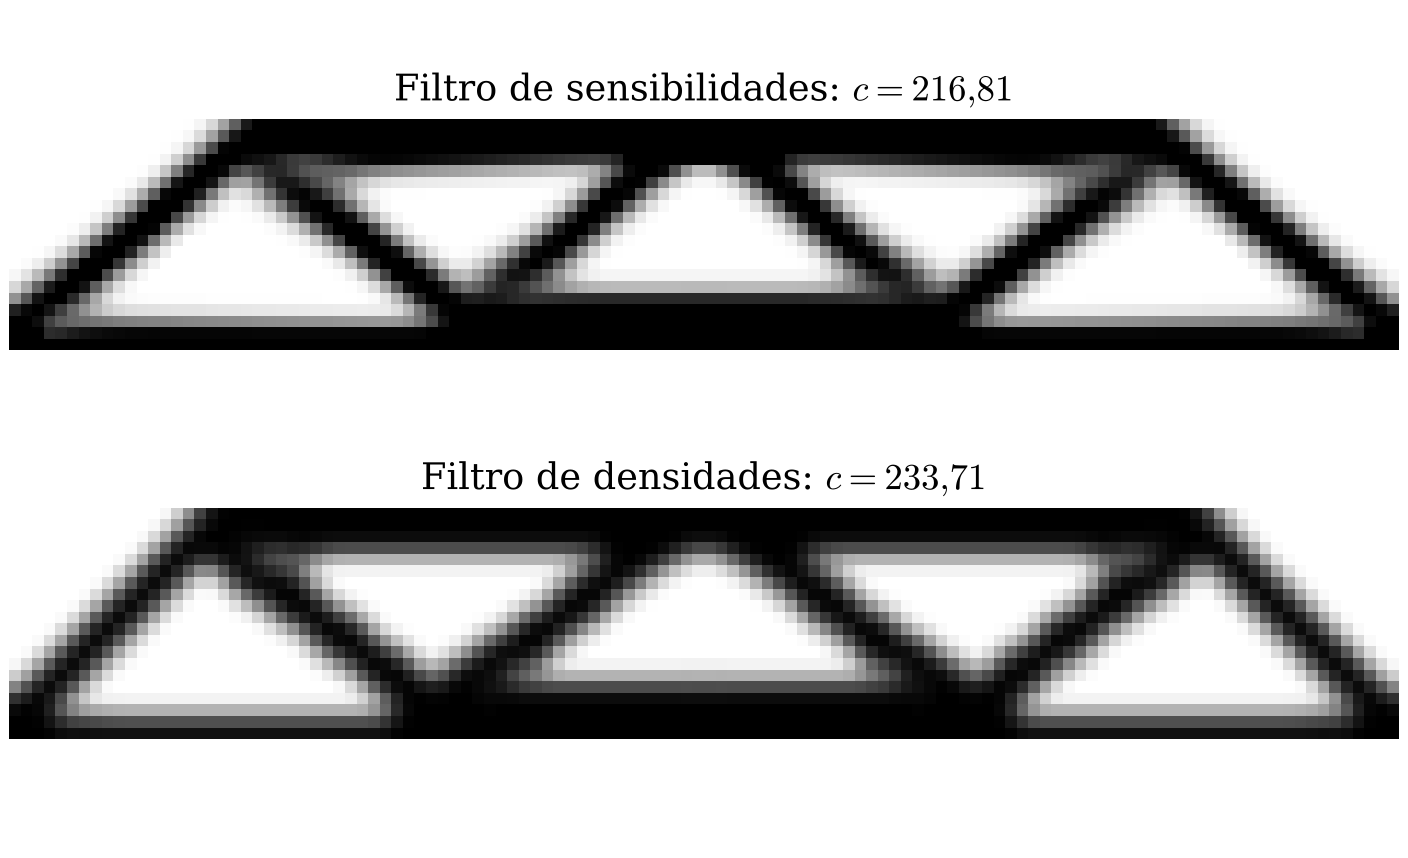
\includegraphics[width=0.82\textwidth]{fig-mbb.png}
\caption{Diseños de la viga MBB completa (semimodelo de $60\times 20$ elementos reflejado), $f_V=0{,}5$, $p=3$, $\rmin=2{,}4$. Negro: material. Calculado con el cuaderno del módulo.}
\label{fig:mbb}
\end{figure}

\section{Fabricación aditiva y diseño generativo}

Un diseño optimizado solo es útil si se puede fabricar. Las restricciones más comunes son el tamaño mínimo de las barras y de los huecos, que el radio del filtro controla; la dirección de fabricación, porque en fabricación aditiva las superficies que miran hacia abajo con poca inclinación necesitan soportes (\cref{tema:6}); y, para mecanizado o fundición, la accesibilidad de la herramienta y el desmoldeo. Langelaar propuso un filtro que, capa a capa, solo permite material que esté sostenido por material de la capa inferior, de modo que el resultado es imprimible sin soportes~\cite{langelaar}. Tras optimizar, el flujo habitual es umbralizar $\xf$, extraer la superficie (\emph{marching cubes} o \emph{squares}, \cref{tema:1}), suavizarla, reconstruir una geometría CAD y \emph{volver a verificar} con un análisis de elementos finitos más fino, incluyendo tensiones, que el problema de flexibilidad no controla.

Los programas comerciales de \emph{diseño generativo} empaquetan este flujo. La documentación pública de Autodesk Fusion describe métodos de fabricación seleccionables (sin restricciones, aditiva con dirección de impresión, fresado de 2,5, 3 y 5 ejes, corte en 2 ejes y fundición con espesor mínimo, ángulo de desmoldeo y dirección de expulsión), cada uno de los cuales genera su propio conjunto de resultados~\cite{fusiongd}. El caso publicado más citado es el soporte de cinturón de un asiento de General Motors: según Autodesk, el diseño generativo consolidó ocho piezas en una sola de acero inoxidable, un 40~\% más ligera y un 20~\% más resistente que la anterior~\cite{gmautodesk}. nTop combina el modelado implícito con resultados de optimización de topología y con campos que modulan celosías y espesores~\cite{ntop}. No se han publicado los algoritmos internos de estos productos.

\begin{table}[h]
\centering\small
\begin{tabularx}{\textwidth}{@{}l>{\raggedright\arraybackslash}X>{\raggedright\arraybackslash}p{2.7cm}>{\raggedright\arraybackslash}X@{}}
\toprule
Herramienta & Para qué sirve & Licencia o tipo & Cuándo elegirla \\
\midrule
top88 y variantes (DTU) & códigos didácticos SIMP en MATLAB & descarga gratuita (DTU) & aprender y prototipar en 2D \\
numpy + scipy.sparse & montaje y resolución de elementos finitos & BSD & reproducir top88 en Python (cuaderno) \\
NLopt (MMA) & optimización con muchas restricciones & MIT & sustituir OC cuando hay varias restricciones \\
dolfin-adjoint & adjuntos automáticos sobre FEniCS & LGPL & EDP generales en 2D y 3D sin derivar a mano \\
Autodesk Fusion & diseño generativo con restricciones de fabricación & comercial & ingeniería de producto con CAD integrado \\
nTop & modelado implícito, celosías, campos & comercial & piezas para fabricación aditiva con celosías \\
\bottomrule
\end{tabularx}
\caption{Tecnologías del tema~2.}
\label{tab:tec2}
\end{table}

\begin{observacion}[Errores frecuentes en la práctica]\label{obs:errores2}
(i) \emph{No filtrar}: aparecen tableros de ajedrez y el resultado depende de la malla. (ii) \emph{Presentar $x$ en lugar de $\xf$} con el filtro de densidades: el diseño mostrado no es el analizado. (iii) \emph{$\Emin=0$}: $K$ se vuelve singular en cuanto un elemento se vacía. (iv) \emph{Confundir rigidez con resistencia}: mínima flexibilidad no garantiza tensiones admisibles; hay que comprobarlas, sobre todo en esquinas entrantes. (v) \emph{Mínimos locales}: con $p=3$ el resultado depende de los parámetros; conviene la continuación en $p$ y comparar varias ejecuciones. (vi) \emph{Olvidar la fabricación}: voladizos, cavidades cerradas que atrapan polvo o resina y espesores inferiores a la resolución de la máquina. (vii) \emph{Coste}: en 3D, la resolución de $KU=F$ domina; se necesitan resolvedores iterativos con precondicionadores multimalla para pasar de unos miles a millones de elementos.
\end{observacion}

\begin{lecturas}
\item M.~P. Bendsøe y O.~Sigmund~\cite{bs}, cap.~1 «Topology optimization by distribution of isotropic material».
\item E.~Andreassen \emph{et al.}~\cite{andreassen}: §2 (formulación, SIMP modificado, OC y filtros) y §3 (implementación).
\item O.~Sigmund y J.~Petersson~\cite{sigpet}: tableros de ajedrez, dependencia de la malla y mínimos locales.
\item P.~Bright, A.~Edelman y S.~G. Johnson~\cite{mit18s096}, §6.3 «Reverse-mode “adjoint” differentiation».
\item M.~Langelaar~\cite{langelaar}: restricciones de voladizo para fabricación aditiva.
\end{lecturas}

\section*{Ejercicios del tema 2}
\addcontentsline{toc}{section}{Ejercicios del tema 2}

\begin{ejercicio}{1}{eje:2-vf}
Justifique si son verdaderas o falsas: (a) con $p=1$ el diseño óptimo suele ser blanco y negro; (b) $\Emin>0$ evita que $K$ sea singular; (c) minimizar la flexibilidad equivale a minimizar la flecha en todos los puntos; (d) el filtro de sensibilidades calcula el gradiente exacto de una función filtrada.
\end{ejercicio}

\begin{ejercicio}{1}{eje:2-gd}
Explique por qué el resultado de un programa de diseño generativo debe volver a analizarse por elementos finitos antes de fabricarlo, y cite dos comprobaciones que el problema de flexibilidad mínima no incluye.
\end{ejercicio}

\begin{ejercicio}{2}{eje:2-penal}
Para $x_e=0{,}5$, calcule la relación rigidez/volumen $E_e/(E_0x_e)$ con $p=1,2,3$ ($\Emin\approx 0$). ¿Qué densidad necesita un elemento con $p=3$ para aportar la mitad de la rigidez del sólido?
\end{ejercicio}

\begin{ejercicio}{2}{eje:2-oc}
Tres elementos con $x=(0{,}5;\ 0{,}5;\ 0{,}5)$, sensibilidades $\partial c/\partial x=(-4;\ -1;\ -0{,}25)$, $\partial V/\partial x_e=1$, $\eta=1/2$, $m=0{,}2$ y volumen objetivo $1{,}5$. Aplique la \cref{def:oc} y encuentre el valor de $\Lambda$ que cumple el volumen.
\end{ejercicio}

\begin{ejercicio}{2}{eje:2-filtro}
En una malla regular con $\rmin=1{,}5$ y densidades uniformes $x_i=0{,}5$, el elemento central de un bloque $3\times 3$ tiene sensibilidad $-4$; sus cuatro vecinos laterales, $-2$, y sus cuatro vecinos diagonales, $-1$. Calcule la sensibilidad filtrada del elemento central.
\end{ejercicio}

\begin{ejercicio}{2}{eje:2-cadena}
Una fila de tres elementos con $\rmin=1{,}5$ (peso propio $1{,}5$ y peso $0{,}5$ para los vecinos inmediatos) y $x=(1;\ 0{,}5;\ 0)$. Calcule las densidades físicas $\xf$ y, si $\partial c/\partial\xf=(-3;\ -2;\ -1)$, las sensibilidades respecto a $x$. Compruebe que la suma de sensibilidades se conserva.
\fuente{adaptado de IUPUI ME 60602 «Topology Optimization» (A.~Tovar), clase~12 «Well-posedness, numerical problems, filters»~\cite{tovar}.}
\end{ejercicio}

\begin{ejercicio}{2}{eje:2-fisico}
El resultado adimensional $\bar c=216{,}81$ de la viga MBB se fabrica en acero ($E_0=200$ GPa, densidad $7{,}85$ g/cm³) con espesor $t=5$ mm, elementos de 1 mm y una carga de 2 kN en el semimodelo. Calcule la flexibilidad física, la flecha bajo la carga y la masa del semimodelo.
\end{ejercicio}

\begin{ejercicio}{3}{eje:2-mecanismo}
En un mecanismo flexible se quiere maximizar el desplazamiento de un nodo de salida, $g=L^\T U$, con $L$ el vector canónico de ese grado de libertad. (a) Escriba el problema adjunto y la sensibilidad $dg/dx_e$ con el \cref{teo:adjunto}. ¿Cuántas resoluciones cuesta el gradiente? (b) Compruébelo en el sistema de dos muelles en serie del \cref{ej:serie} tomando como salida el nodo intermedio, $g=u_1$, cuyo valor exacto es $F/k_1$.
\fuente{adaptado de MIT 18.S096 «Matrix Calculus for Machine Learning and Beyond» (A.~Edelman y S.~G. Johnson, IAP 2023), §6.3 «Reverse-mode “adjoint” differentiation»~\cite{mit18s096}.}
\end{ejercicio}

\begin{ejercicio}{3}{eje:2-kkt}
(a) Demuestre que en el problema de la \cref{def:compliance} con SIMP se cumple $\partial c/\partial x_e\le 0$ y deduzca que en un óptimo con $0<x_e<1$ para algún $e$ la restricción de volumen puede tomarse como desigualdad activa $\sum_ex_e\le Nf_V$. (b) Escriba las condiciones de Karush--Kuhn--Tucker con las cotas $0\le x_e\le 1$ y deduzca que, para los elementos interiores, $B_e=1$, y que en los elementos con $x_e=1$ se cumple $B_e\ge 1$.
\fuente{adaptado de M.~P. Bendsøe y O.~Sigmund, \emph{Topology Optimization}, cap.~1~\cite{bs}.}
\end{ejercicio}

% =====================================================================
\chapter{Simuladores diferenciables y modelos sustitutos}
\label{tema:3}
% =====================================================================

El \cref{tema:2} obtuvo el gradiente de un simulador de elementos finitos derivando a mano sus ecuaciones. Este tema generaliza la idea a cualquier simulador, estacionario o temporal, y presenta la alternativa cuando derivar no es posible o el simulador es demasiado caro: aprender un modelo sustituto con pocas simulaciones y optimizar sobre él. Se siguen las notas de S.~G. Johnson sobre adjuntos para recurrencias~\cite{johnson}, las de cálculo matricial del MIT~\cite[§6.3]{mit18s096}, los capítulos de modelos sustitutos de Kochenderfer y Wheeler~\cite{kw}, y los artículos de DiffTaichi~\cite{difftaichi}, las redes informadas por la física~\cite{pinn}, el operador neuronal de Fourier~\cite{fno} y MeshGraphNets~\cite{mgn}. La física de la aleta procede del capítulo~3 de Incropera \emph{et al.}~\cite{incropera}.

\section{Derivar a través de un simulador}

Casi todo simulador discreto resuelve un sistema de ecuaciones $R(u,\theta)=0$, donde $u\in\R^m$ es el estado (temperaturas, desplazamientos, velocidades) y $\theta\in\R^n$ son los parámetros de diseño.

\begin{teorema}[Sensibilidad por la función implícita y el adjunto]\label{teo:implicita}
Sean $R:\R^m\times\R^n\to\R^m$ y $J(\theta)=g\bigl(u(\theta),\theta\bigr)$ funciones continuamente derivables, con $R(u(\theta),\theta)=0$ y $\partial R/\partial u$ invertible en la solución. Entonces
\[
\frac{du}{d\theta}=-\Bigl(\frac{\partial R}{\partial u}\Bigr)^{-1}\frac{\partial R}{\partial\theta},\qquad
\frac{dJ}{d\theta}=\frac{\partial g}{\partial\theta}-\lambda^\T\frac{\partial R}{\partial\theta},\quad\text{con}\quad\Bigl(\frac{\partial R}{\partial u}\Bigr)^{\!\T}\lambda=\Bigl(\frac{\partial g}{\partial u}\Bigr)^{\!\T}.
\]
\end{teorema}

\begin{proof}
El teorema de la función implícita garantiza que $u(\theta)$ es derivable cerca de la solución. Derivando la identidad $R(u(\theta),\theta)=0$ se obtiene $\frac{\partial R}{\partial u}\frac{du}{d\theta}+\frac{\partial R}{\partial\theta}=0$, de donde sale la primera fórmula. Sustituyéndola en $\frac{dJ}{d\theta}=\frac{\partial g}{\partial\theta}+\frac{\partial g}{\partial u}\frac{du}{d\theta}$ y agrupando $\frac{\partial g}{\partial u}\bigl(\frac{\partial R}{\partial u}\bigr)^{-1}=\lambda^\T$ se obtiene la segunda.
\end{proof}

El \cref{teo:adjunto} es el caso $R=K(x)U-F$. El coste del adjunto es una resolución con la matriz transpuesta, que en problemas lineales puede reutilizar la factorización ya calculada; el de la sensibilidad directa, $n$ resoluciones. Para simuladores temporales, $u_{k+1}=\Phi(u_k,\theta)$, el mismo razonamiento da una recurrencia adjunta que se recorre hacia atrás en el tiempo~\cite{johnson}:
\[
\lambda_N=\Bigl(\frac{\partial g}{\partial u_N}\Bigr)^{\!\T},\qquad \lambda_{k-1}=\Bigl(\frac{\partial\Phi}{\partial u}\Bigr)^{\!\T}_{\!k}\lambda_k,\qquad \frac{dg}{d\theta}=\frac{\partial g}{\partial\theta}+\sum_{k=1}^N\lambda_k^\T\frac{\partial\Phi}{\partial\theta}\Big|_{u_{k-1}} .
\]
Es la retropropagación a través del tiempo de una red recurrente (módulo~12, §5.3), con los mismos problemas: hay que guardar todos los estados, lo que se alivia con el recálculo por puntos de control (módulo~10, §5.2), y en dinámicas caóticas o con muchos pasos el gradiente puede explotar.

\section{Diferenciación automática de simuladores}

En lugar de derivar a mano, el simulador se puede escribir en un lenguaje que propague derivadas. JAX transforma programas de Python y NumPy (derivación, vectorización y compilación para GPU y TPU)~\cite{jax}; NVIDIA Warp compila núcleos de Python para GPU que son derivables~\cite{warp}; Taichi, con su extensión DiffTaichi, permite escribir simuladores físicos derivables, y sus autores informan de que su simulador elástico necesita unas 4,2 veces menos líneas que una versión CUDA escrita a mano, con velocidad similar, y es 188 veces más rápido que la implementación en TensorFlow~\cite{difftaichi}. PyTorch también sirve cuando el simulador se expresa con operaciones de tensores, como en el caso de estudio de este tema.

Tres advertencias limitan el enfoque. Los eventos discretos (contactos, cambios de malla, condicionales sobre el estado) producen funciones discontinuas cuya derivada automática es correcta pero inútil, porque vale cero o no ve el salto. Las derivadas de un resolvedor iterativo no deben calcularse a través de sus iteraciones, sino con el \cref{teo:implicita} en la solución convergida. Y el coste de memoria del modo inverso crece con el número de pasos de tiempo.

\section{Modelos sustitutos}

\begin{definicion}[Modelo sustituto]\label{def:sustituto}
Sea $s:\Theta\to\R$ una respuesta cara de evaluar (el resultado de un simulador). Un \emph{modelo sustituto} es una función $\hat s_\varphi$ barata, ajustada con un conjunto de diseño $\{(\theta_i,s(\theta_i))\}_{i=1}^M$, con la que se sustituye a $s$ dentro de la optimización.
\end{definicion}

Los sustitutos clásicos son las superficies de respuesta polinómicas ajustadas por mínimos cuadrados y los procesos gaussianos, que además estiman su incertidumbre~\cite{kw}. Los neuronales cubren desde un perceptrón que aproxima una respuesta escalar hasta modelos que aproximan campos completos: las redes informadas por la física (PINN) minimizan el residuo de la ecuación diferencial en puntos de colocación, calculando las derivadas de la red por diferenciación automática~\cite{pinn}; los operadores neuronales de Fourier aprenden la aplicación entre funciones de entrada y de salida, y sus autores informan de aceleraciones de hasta tres órdenes de magnitud frente a resolvedores clásicos~\cite{fno}; MeshGraphNets aprende la dinámica sobre la malla de simulación con una red de grafos~\cite{mgn}. Bibliotecas como NVIDIA PhysicsNeMo (antes Modulus) agrupan estas arquitecturas para construir sustitutos de CFD, mecánica estructural o análisis térmico~\cite{physicsnemo}.

El diseño de experimentos importa tanto como el modelo. El muestreo por hipercubo latino divide el rango de cada variable en $M$ intervalos y toma exactamente una muestra por intervalo, de modo que sus proyecciones sobre cada eje quedan uniformemente repartidas~\cite{kw}.

\begin{proposicion}[Error del óptimo de un sustituto]\label{prop:2eps}
Sea $\Theta$ compacto, $s$ y $\hat s$ continuas y $\sup_{\theta\in\Theta}\abs{\hat s(\theta)-s(\theta)}\le\varepsilon$. Si $\theta^\star$ minimiza $s$ y $\hat\theta$ minimiza $\hat s$ en $\Theta$, entonces
\[
s(\theta^\star)\le s(\hat\theta)\le s(\theta^\star)+2\varepsilon .
\]
\end{proposicion}

\begin{proof}
La primera desigualdad es la optimalidad de $\theta^\star$. Para la segunda, $s(\hat\theta)\le\hat s(\hat\theta)+\varepsilon\le\hat s(\theta^\star)+\varepsilon\le s(\theta^\star)+2\varepsilon$, usando sucesivamente la cota de error, la optimalidad de $\hat\theta$ para $\hat s$ y otra vez la cota.
\end{proof}

La proposición es tranquilizadora y peligrosa a la vez: la garantía exige un error \emph{uniforme} en todo $\Theta$, mientras que la validación solo mide el error en unos puntos. El optimizador busca precisamente las zonas en que $\hat s$ es optimista, que suelen ser aquellas en que hay pocos datos. Es el mismo fenómeno que la sobreoptimización de un modelo de recompensa (módulo~21, §6.4). Por eso todo diseño propuesto por un sustituto se verifica con el simulador y, si hay presupuesto, se añade a los datos y se reajusta el modelo.

\section{Caso de estudio: el perfil de una aleta disipadora}

\begin{ejemplo}[Aleta de aluminio con sustituto neuronal y con simulador diferenciable]\label{ej:aleta}
\emph{Contexto.} Un disipador de aluminio ($k=200$ W/(m·K)) refrigerado por aire forzado ($h=60$ W/(m²·K)) debe evacuar calor desde una base a $\theta_b=T_b-T_\infty=50$ K. La masa de cada aleta está fijada: por cada metro de profundidad, el área del perfil es $A=60$ mm². El perfil es trapecial, con espesor $t(x)=t_b(1-s\,x/L)$ para $0\le x\le L$, donde $L$ es la longitud y $s\in[0,1)$ la conicidad; la condición de área fija da $t_b=A/\bigl(L(1-s/2)\bigr)$. Por extrusión, la punta debe medir al menos $t_{\min}=0{,}3$ mm.

\emph{Modelo físico.} Con aleta delgada (número de Biot $ht/(2k)\ll 1$), conducción longitudinal y convección por las dos caras, la temperatura $\theta(x)$ por metro de profundidad satisface~\cite{incropera}
\[
\frac{d}{dx}\Bigl(k\,t(x)\,\frac{d\theta}{dx}\Bigr)-2h\,\theta=0,\qquad \theta(0)=\theta_b,\qquad \theta'(L)=0,
\]
y el calor evacuado es $q=2h\int_0^L\theta\,dx$. Para $s=0$ hay solución cerrada, $q=\sqrt{2hkt}\,\theta_b\tanh(mL)$ con $m=\sqrt{2h/(kt)}$.

\emph{Formulación.}
\[
\max_{L,\,s}\ q(L,s)\quad\text{sujeto a}\quad t_b(1-s)\ge t_{\min},\quad 20\le L\le 100\ \text{mm},\quad 0\le s\le 0{,}9 .
\]
El simulador discretiza la ecuación por volúmenes finitos con 400 celdas y resuelve un sistema tridiagonal; reproduce la solución cerrada de la aleta rectangular con un error relativo de $1{,}4\cdot 10^{-6}$.

\emph{Línea base.} Para $s=0$, el óptimo con área fija cumple $\sinh(2\beta)=6\beta$ con $\beta=mL$ (\cref{eje:3-schmidt}), es decir, $\beta=1{,}4192$. Con los datos, $L=58{,}6$ mm, $t=1{,}02$ mm y $q=220{,}4$ W/m: unos 11 W para una aleta de 50 mm de profundidad.

\emph{Método 1: sustituto neuronal.} Se supone que cada simulación es cara (en un diseño real sería un cálculo CFD conjugado de horas) y se dispone de 40. Se toman 60 puntos por hipercubo latino en $(L,s)$, se descartan los no fabricables y se simulan los 40 primeros factibles. Un perceptrón 2--32--32--1 con activación tanh, entrenado con 32 puntos, tiene un error cuadrático medio de 10,1 W/m (4,9~\% de la media) en los 8 reservados. Reentrenado con los 40, su máximo en una rejilla factible de $201\times 201$ está en $L=62{,}4$ mm y $s=0{,}815$, con predicción de 242,2 W/m; la simulación de verificación (la número 41) da 242,0 W/m.

\emph{Método 2: simulador diferenciable.} El mismo simulador escrito con tensores de PyTorch (200 celdas, sistema denso) da $\partial q/\partial L$ y $\partial q/\partial s$ por diferenciación automática, que coinciden con diferencias finitas centradas en seis cifras. Ascenso de gradiente con Adam (módulo~7, §5.3) y \emph{proyección} sobre la restricción de la punta, $s\le s_{\max}(L)=(1-r)/(1-r/2)$ con $r=t_{\min}L/A$, converge en 150 iteraciones a $L=66{,}3$ mm y $s=0{,}801$, con $q=242{,}2$ W/m y la restricción activa (punta de 0,300 mm).

\emph{Comprobación y conclusión.} Una búsqueda exhaustiva en $81\times 96$ puntos (7776 simulaciones) da $q=242{,}1$ W/m en $L=66$ mm y $s=0{,}80$. Los dos métodos llegan a menos del 0,1~\% de ese valor y mejoran la aleta rectangular óptima en un 9,8~\% con la misma masa. El óptimo está sobre la restricción de fabricación: si se pudiera hacer la punta más fina, la aleta mejoraría hacia el perfil triangular. El sustituto encontró una solución algo distinta ($L=62$ mm) con casi el mismo calor porque la función es muy plana cerca del óptimo; el método del gradiente necesita el simulador derivable, pero no un presupuesto de muestras.
\end{ejemplo}

\begin{table}[h]
\centering\small
\begin{tabularx}{\textwidth}{@{}l>{\raggedright\arraybackslash}X>{\raggedright\arraybackslash}p{2.3cm}>{\raggedright\arraybackslash}X@{}}
\toprule
Herramienta & Para qué sirve & Licencia & Cuándo elegirla \\
\midrule
JAX & derivación, vectorización y compilación de código NumPy & Apache-2.0 & simuladores nuevos escritos en estilo funcional \\
NVIDIA Warp & núcleos de simulación derivables en GPU & Apache-2.0 & física de partículas, telas o sólidos en GPU \\
Taichi (DiffTaichi) & lenguaje para simulación física derivable & Apache-2.0 & simuladores de partículas y rejillas de alto rendimiento \\
PyTorch & tensores y diferenciación automática & BSD-3 (con componentes de otras licencias) & simuladores pequeños unidos a redes neuronales \\
NVIDIA PhysicsNeMo & PINN, operadores neuronales y GNN para física & Apache-2.0 & sustitutos de CFD o de estructuras a escala industrial \\
scikit-learn & MLP, procesos gaussianos, validación & BSD-3 & sustitutos de pocas variables con pocos datos \\
dolfin-adjoint & adjuntos automáticos de modelos FEniCS & LGPL & EDP generales con elementos finitos \\
\bottomrule
\end{tabularx}
\caption{Tecnologías del tema~3. Licencias según los metadatos publicados por cada proyecto.}
\label{tab:tec3}
\end{table}

\begin{observacion}[Errores frecuentes en la práctica]\label{obs:errores3}
(i) \emph{Sobreajuste del sustituto}: con 40 puntos y miles de pesos, la red interpola el ruido; hay que reservar datos de validación y regularizar. (ii) \emph{Extrapolación}: el optimizador lleva el diseño a los bordes del dominio, donde hay menos datos; se verifica siempre con el simulador (\cref{prop:2eps}). (iii) \emph{Fugas de datos}: si los puntos de validación son casi idénticos a los de entrenamiento (simulaciones repetidas con otra malla, por ejemplo), el error de validación es optimista. (iv) \emph{La verdad tampoco es exacta}: el simulador tiene error de discretización; hay que comprobar la convergencia de malla antes de entrenar con él. (v) \emph{Validez del modelo físico}: el caso supone aleta delgada; con $ht/k$ grande o radiación apreciable, el modelo unidimensional no vale. (vi) \emph{Restricciones de seguridad}: un sustituto puede predecir un diseño factible que no lo es; las restricciones críticas se comprueban con el simulador o con un margen. (vii) \emph{Coste mal contado}: el entrenamiento del sustituto y las simulaciones de verificación forman parte del presupuesto.
\end{observacion}

\begin{lecturas}
\item M.~J. Kochenderfer y T.~A. Wheeler~\cite{kw}: caps. «Sampling Plans», «Surrogate Models», «Probabilistic Surrogate Models» y «Surrogate Optimization».
\item S.~G. Johnson~\cite{johnson}: adjuntos para relaciones de recurrencia (MIT 18.335J).
\item Y.~Hu \emph{et al.}~\cite{difftaichi}: programación diferenciable para simulación física.
\item M.~Raissi, P.~Perdikaris y G.~E. Karniadakis~\cite{pinn}; Z.~Li \emph{et al.}~\cite{fno}; T.~Pfaff \emph{et al.}~\cite{mgn}.
\item F.~P. Incropera \emph{et al.}~\cite{incropera}, cap.~3: conducción unidimensional y superficies extendidas.
\end{lecturas}

\section*{Ejercicios del tema 3}
\addcontentsline{toc}{section}{Ejercicios del tema 3}

\begin{ejercicio}{1}{eje:3-elegir}
Para cada caso, elija entre sustituto, simulador diferenciable o diferencias finitas y justifíquelo: (a) 3 parámetros y un CFD comercial de cajas negras que tarda 6 horas; (b) 5000 densidades y un código de elementos finitos propio; (c) un simulador de choques con contactos y 20 parámetros.
\end{ejercicio}

\begin{ejercicio}{1}{eje:3-pinn}
Escriba la pérdida de una red informada por la física $\theta_\varphi(x)$ para la aleta rectangular del \cref{ej:aleta}: identifique el término de residuo y los de condiciones de contorno, y explique por qué no hace falta malla.
\end{ejercicio}

\begin{ejercicio}{2}{eje:3-aleta}
Para una aleta rectangular de $L=40$ mm y $t=1{,}5$ mm ($A=60$ mm²), con los datos del \cref{ej:aleta}, calcule $m$, $mL$, el calor $q$, la eficiencia $\eta=\tanh(mL)/(mL)$ y el número de Biot $ht/(2k)$.
\fuente{adaptado de F.~P. Incropera \emph{et al.}, \emph{Fundamentals of Heat and Mass Transfer}, cap.~3 (aletas de sección uniforme)~\cite{incropera}.}
\end{ejercicio}

\begin{ejercicio}{2}{eje:3-coste}
La viga MBB tiene 1200 variables y cada resolución de $KU=F$ tarda 10 ms. Compare el tiempo de calcular el gradiente por diferencias finitas hacia delante y por el método adjunto, y el de 100 iteraciones de optimización con cada uno.
\end{ejercicio}

\begin{ejercicio}{2}{eje:3-implicita}
Sea $R(u,\theta)=A(\theta)u-b$ con $A(\theta)=\begin{psmallmatrix}2+\theta&-1\\-1&2\end{psmallmatrix}$, $b=(1,0)^\T$ y $J=u_1+u_2$. En $\theta=0$, calcule $u$, el vector adjunto $\lambda$ y $dJ/d\theta$, y compruébelo con una diferencia finita de paso $0{,}01$.
\end{ejercicio}

\begin{ejercicio}{2}{eje:3-cuadratico}
Se simula la aleta rectangular del \cref{ej:aleta} en $L=30$, 60 y 90 mm, con resultados $q=165{,}38$; $220{,}34$ y $198{,}20$ W/m. Ajuste un sustituto cuadrático $\hat q(L)=\beta_0+\beta_1L+\beta_2L^2$ ($L$ en mm), calcule su máximo y compárelo con el óptimo verdadero ($L=58{,}6$ mm, $q=220{,}42$ W/m), sabiendo que el simulador da $218{,}13$ W/m en el máximo del sustituto.
\fuente{adaptado de M.~J. Kochenderfer y T.~A. Wheeler, \emph{Algorithms for Optimization}, cap. «Surrogate Models»~\cite{kw}.}
\end{ejercicio}

\begin{ejercicio}{2}{eje:3-recurrencia}
Un componente se enfría según $\theta_{k+1}=(1-a\Delta t)\,\theta_k$ con $\theta_0=50$ K, $\Delta t=1$ s y $a=0{,}1$ s$^{-1}$. Calcule $\theta_3$ y $d\theta_3/da$ derivando la expresión cerrada y con la recurrencia adjunta hacia atrás.
\fuente{adaptado de S.~G. Johnson, «Adjoint methods and sensitivity analysis for recurrence relations», notas de MIT 18.335J (otoño de 2010)~\cite{johnson}.}
\end{ejercicio}

\begin{ejercicio}{3}{eje:3-cota}
(a) Demuestre la \cref{prop:2eps}. (b) Construya un ejemplo con $\Theta=[0,1]$ en el que el sustituto tenga error nulo en tres puntos de validación y, sin embargo, su minimizador sea pésimo para $s$. ¿Qué enseña sobre la validación de sustitutos?
\end{ejercicio}

\begin{ejercicio}{3}{eje:3-schmidt}
(a) Demuestre que, para la aleta rectangular de área de perfil fija $A$, el calor $q(L)=\sqrt{2hkA/L}\,\theta_b\tanh\bigl(c\,L^{3/2}\bigr)$, con $c=\sqrt{2h/(kA)}$, es máximo cuando $\beta=cL^{3/2}$ cumple $\sinh(2\beta)=6\beta$. (b) Con $h=40$ W/(m²·K), $k=170$ W/(m·K), $A=50$ mm² y $\theta_b=50$ K, calcule $L$, $t$ y $q$ óptimos, usando $\beta=1{,}4192$.
\end{ejercicio}

% =====================================================================
\chapter{Renderizado diferenciable y reconstrucción 3D}
\label{tema:4}
% =====================================================================

Reconstruir un objeto a partir de fotografías es un problema inverso: se busca la geometría (y la apariencia) cuyas imágenes renderizadas coinciden con las observadas. Si el renderizador es derivable, el problema se resuelve por descenso de gradiente, igual que el entrenamiento de una red. Este tema explica por qué la rasterización clásica no es derivable, cómo la suavizan SoftRas~\cite{softras} y las bibliotecas actuales~\cite{pytorch3d,nvdiffrast,mitsuba3}, y cómo NeRF~\cite{nerf} y el \emph{Gaussian splatting}~\cite{gs} convierten la reconstrucción de escenas en una optimización. Se apoya en las clases «Graphics Pipeline and Rasterization» de MIT 6.837~\cite{mit6837}, en la clase de renderizado neuronal de CS348n~\cite{cs348n} y en las tareas~2 y~3 del curso 16-825 de Carnegie Mellon~\cite{cmu16825}.

\section{Formación de la imagen y rasterización}

Una cámara estenopeica con matriz de rotación $W$, centro $o$ y distancia focal $\phi$ (en píxeles) proyecta el punto $X$ en el píxel $\bigl(\phi\,X_c^{(1)}/X_c^{(3)},\ \phi\,X_c^{(2)}/X_c^{(3)}\bigr)$, con $X_c=W(X-o)$. La rasterización recorre los triángulos proyectados y asigna a cada píxel el triángulo más cercano que lo cubre (\emph{z-buffer})~\cite{mit6837}. La silueta de una malla es la función indicadora de los píxeles cubiertos.

\begin{proposicion}[La rasterización tiene gradiente nulo casi en todas partes]\label{prop:grad-cero}
Sea $I_p(\theta)\in\{0,1\}$ el valor de la silueta en el píxel $p$ (muestreado en su centro) como función de las coordenadas $\theta$ de los vértices. Entonces $I_p$ es constante a trozos: en todo $\theta$ en que ningún borde de triángulo proyectado pasa exactamente por el centro de $p$, $\nabla_\theta I_p=0$.
\end{proposicion}

\begin{proof}
La pertenencia del centro del píxel a un triángulo proyectado se decide con los signos de tres funciones de arista, continuas en $\theta$. Si ninguna se anula, sus signos se conservan en un entorno de $\theta$ y la cobertura no cambia, así que $I_p$ es constante en ese entorno. Los puntos en que alguna se anula forman un conjunto de medida nula.
\end{proof}

Una pérdida que compare siluetas rasterizadas tiene, por tanto, gradiente nulo salvo en un conjunto de medida nula, donde no existe: el descenso de gradiente no recibe información. Hay dos soluciones: suavizar el renderizador, o calcular explícitamente la contribución de los bordes (como hacen los métodos de antialias derivable de nvdiffrast~\cite{nvdiffrast} y los renderizadores físicos como Mitsuba~3~\cite{mitsuba3}).

\section{Rasterización suave}

\begin{definicion}[Mapa de probabilidad de SoftRas]\label{def:softras}
Para el píxel $p_i$ y el triángulo proyectado $f_j$, SoftRas~\cite[§3.2]{softras} define
\[
D_j^i=\sigm\Bigl(\delta_j^i\,\frac{d^2(i,j)}{\sigma}\Bigr),
\]
donde $d(i,j)$ es la distancia del píxel al borde del triángulo, $\delta_j^i=+1$ si el píxel está dentro y $-1$ si está fuera, y $\sigma>0$ controla la nitidez. La silueta suave se obtiene agregando los triángulos como sucesos independientes~\cite[§3.3]{softras},
\[
I_s^i=1-\prod_j\bigl(1-D_j^i\bigr).
\]
\end{definicion}

Cuando $\sigma\to 0$, $D_j^i$ tiende a la indicadora del triángulo y se recupera la rasterización clásica; con $\sigma>0$, todos los triángulos cercanos reciben gradiente, incluso los ocultos y los vértices alejados del borde. El valor por defecto en el artículo es $\sigma=10^{-4}$ en coordenadas de imagen normalizadas. La pérdida de siluetas más usada es $1-\IoU$ suave, con $\IoU(S,T)=\sum_iS_iT_i/\sum_i(S_i+T_i-S_iT_i)$~\cite[§4.1]{softras}. El compromiso es claro: un $\sigma$ grande da gradientes en una región amplia, útiles al principio, pero sesga la silueta (la «hincha»); un $\sigma$ pequeño es fiel pero casi no da gradiente. De ahí la práctica de \emph{recocer} $\sigma$ de grande a pequeño, que se ve en el caso de estudio.

Las bibliotecas actuales implementan estas ideas con eficiencia. PyTorch3D proporciona estructuras de mallas y nubes por lotes, pérdidas 3D y un renderizador derivable modular~\cite{pytorch3d}. nvdiffrast ofrece primitivas de alto rendimiento (rasterización, interpolación de atributos, filtrado de texturas y antialias) que aprovechan el hardware gráfico y se integran en PyTorch o TensorFlow~\cite{nvdiffrast}. Mitsuba~3, construido sobre el compilador Dr.Jit, calcula derivadas de simulaciones completas de transporte de luz respecto a la cámara, la geometría, los materiales o las texturas~\cite{mitsuba3}.

\section{Renderizado volumétrico y NeRF}

Un campo de radiancia neuronal (NeRF) representa una escena con una red que, para cada punto $X$ y dirección de vista $d$, devuelve una densidad $\sigma(X)\ge 0$ y un color $c(X,d)$~\cite{nerf}. El color de un rayo $r(t)=o+td$ es
\[
C(r)=\int_{t_n}^{t_f}T(t)\,\sigma(r(t))\,c(r(t),d)\,dt,\qquad T(t)=\exp\Bigl(-\int_{t_n}^{t}\sigma(r(u))\,du\Bigr),
\]
donde $T(t)$ es la transmitancia, la probabilidad de que la luz recorra el rayo hasta $t$ sin ser absorbida. Con muestras $t_1<\dots<t_N$ y $\delta_i=t_{i+1}-t_i$, la cuadratura de NeRF~\cite[§4]{nerf} es
\[
\hat C(r)=\sum_{i=1}^N w_i\,c_i,\qquad w_i=T_i\,\alpha_i,\qquad \alpha_i=1-e^{-\sigma_i\delta_i},\qquad T_i=\exp\Bigl(-\sum_{j<i}\sigma_j\delta_j\Bigr)=\prod_{j<i}(1-\alpha_j).
\]

\begin{proposicion}[Los pesos del rayo]\label{prop:pesos}
Con $\sigma_i\ge 0$, los pesos cumplen $w_i\ge 0$ y $\sum_{i=1}^Nw_i=1-T_{N+1}\le 1$, donde $T_{N+1}=\prod_{j\le N}(1-\alpha_j)$ es la transmitancia residual.
\end{proposicion}

\begin{proof}
Como $\sigma_i\delta_i\ge 0$, se tiene $\alpha_i\in[0,1)$ y $T_i\in(0,1]$, luego $w_i\ge 0$. Además $w_i=T_i\alpha_i=T_i-T_i(1-\alpha_i)=T_i-T_{i+1}$, y la suma es telescópica: $\sum_{i=1}^N(T_i-T_{i+1})=T_1-T_{N+1}=1-T_{N+1}$.
\end{proof}

Los pesos forman, pues, una distribución de probabilidad (completada con el fondo, de peso $T_{N+1}$) sobre el punto del rayo en que la luz se emite; la profundidad esperada es $\sum_iw_it_i$. El renderizado es derivable respecto a $\sigma_i$ y $c_i$, y por tanto respecto a los pesos de la red. NeRF aplica a las coordenadas una codificación posicional $\gamma(p)=\bigl(\sin(2^0\pi p),\cos(2^0\pi p),\dots,\sin(2^{L-1}\pi p),\cos(2^{L-1}\pi p)\bigr)$ con $L=10$ para la posición y $L=4$ para la dirección, una red de 8 capas de 256 unidades, y minimiza el error cuadrático entre colores renderizados y observados con lotes de 4096 rayos; cada escena necesita entre $10^5$ y $3\cdot 10^5$ iteraciones, uno o dos días en una GPU V100~\cite[§5]{nerf}.

\section{\emph{Gaussian splatting}}

El \emph{Gaussian splatting} 3D~\cite{gs} sustituye la red por un conjunto explícito de gaussianas anisótropas, cada una con media $\mu$, covarianza $\Sigma$, opacidad $o$ y color dependiente de la vista (coeficientes de armónicos esféricos). Para que la covarianza siga siendo válida durante la optimización se parametriza como
\[
\Sigma=R\,S\,S^\T R^\T,
\]
con $R$ la rotación de un cuaternión normalizado y $S$ diagonal de escalas~\cite[§4]{gs}. Cada gaussiana se proyecta a la imagen con la covarianza $\Sigma'=JW\Sigma W^\T J^\T$, donde $J$ es el jacobiano de la aproximación afín de la proyección, y las gaussianas que cubren un píxel, ordenadas por profundidad, se componen con la misma fórmula que NeRF:
\[
C=\sum_i c_i\,\alpha_i\prod_{j<i}(1-\alpha_j),\qquad \alpha_i=o_i\exp\Bigl(-\tfrac12(p-\mu_i')^\T\Sigma_i'^{-1}(p-\mu_i')\Bigr).
\]
La pérdida combina $L^1$ y D-SSIM con peso $\lambda=0{,}2$; un control adaptativo clona o divide gaussianas donde el gradiente de posición es grande y elimina las casi transparentes, y un rasterizador por teselas de $16\times 16$ píxeles con ordenación por radix en GPU permite renderizar en tiempo real (al menos 30 fotogramas por segundo a 1080p) escenas de uno a cinco millones de gaussianas~\cite{gs}. Frente a NeRF, el \emph{splatting} cambia una representación implícita y compacta, pero lenta de muestrear, por una explícita, rápida y más voluminosa en memoria.

\section{Caso de estudio: ajuste de una forma a siluetas}

\begin{ejemplo}[Reconstrucción de una pieza a partir de seis siluetas]\label{ej:siluetas}
\emph{Contexto.} Se quiere reconstruir una pieza a partir de fotografías segmentadas (máscaras binarias), por ejemplo para verificar una pieza de fundición o crear un recurso digital. La pieza cabe en un cubo de 40 mm de lado y es estrellada respecto a su centro: su superficie es $\{\rho\,\hx:\rho=r(\hx)\}$ con
\[
r(\hx)=\exp\Bigl(\sum_{\ell=0}^{3}\sum_{m=-\ell}^{\ell}c_{\ell m}\,Y_{\ell m}(\hx)\Bigr),
\]
donde $Y_{\ell m}$ son los armónicos esféricos reales y $\theta=(c_{\ell m})\in\R^{16}$. La exponencial garantiza $r>0$. Hay 6 vistas ortográficas de orientación conocida y aleatoria, de $40\times 40$ píxeles, con 40 muestras por rayo (unidad de longitud: 20 mm).

\emph{Renderizador suave.} La ocupación de un punto $X$ es $o(X)=\sigm\bigl((r(\hx)-\norm{X})/\tau\bigr)$, una versión suave de la indicadora de la pieza, y la silueta de un rayo con muestras $X_1,\dots,X_{40}$ es $S=1-\prod_k\bigl(1-o(X_k)\bigr)$, la agregación de SoftRas (\cref{def:softras}). La base de armónicos de cada muestra se precalcula, de modo que una pasada cuesta un producto de una matriz de $6\cdot 64\,000$ filas por $\theta$.

\emph{Formulación.} $\min_\theta\ 1-\IoU\bigl(S(\theta;\tau),T\bigr)$, con $T$ las seis máscaras binarias; se optimiza con Adam (tasa 0,03, 300 iteraciones) desde una esfera de radio 8 mm.

\emph{Elección del método.} El gradiente de la pérdida respecto a los 16 coeficientes atraviesa la sigmoide de cada muestra; con $\tau$ fijo y pequeño, solo las muestras muy cercanas al contorno aportan, y con $\tau$ grande la silueta suave queda sesgada. Se compara $\tau=0{,}03$ fijo con un recocido geométrico de $\tau$ desde $0{,}05$ hasta $0{,}005$ (de 1 mm a 0,1 mm).

\emph{Resultado.} Con $\tau$ fijo, la $\IoU$ de las siluetas binarias es $0{,}827$ y la $\IoU$ volumétrica (medida en una rejilla de $64^3$) es $0{,}744$: la silueta suave de cada rayo acumula muchas muestras con ocupación intermedia y se hincha, y el optimizador compensa encogiendo la pieza. Con recocido, la $\IoU$ de siluetas es $0{,}995$ y la volumétrica $0{,}991$, y los coeficientes se recuperan con un error relativo inferior al 1~\%. Cada ajuste tarda unos 4 s en una CPU.

\emph{Límite fundamental.} Las siluetas solo determinan el \emph{casco visual} del objeto, la intersección de los conos de visión de sus siluetas~\cite{laurentini}: una concavidad que no se ve de perfil desde ninguna cámara es invisible. Aquí la recuperación es casi perfecta porque la familia de formas (16 coeficientes, armónicos de grado bajo) es pequeña; con formas generales hacen falta términos fotométricos o de profundidad.
\end{ejemplo}

\begin{table}[h]
\centering\small
\begin{tabularx}{\textwidth}{@{}l>{\raggedright\arraybackslash}X>{\raggedright\arraybackslash}p{2.9cm}>{\raggedright\arraybackslash}X@{}}
\toprule
Herramienta & Para qué sirve & Licencia & Cuándo elegirla \\
\midrule
PyTorch3D & rasterización suave de mallas y nubes, pérdidas 3D & BSD & ajuste de mallas e investigación en PyTorch \\
nvdiffrast & primitivas de rasterización derivable de alto rendimiento & licencia de código de NVIDIA & mallas grandes, texturas y antialias en GPU NVIDIA \\
Mitsuba~3 & renderizado físico (transporte de luz) derivable & BSD-3 (con cláusula adicional) & materiales, iluminación indirecta, medios participantes \\
Kaolin & conversiones y renderizado derivable & Apache-2.0 & ecosistema NVIDIA \\
nerfstudio & entrenamiento modular de NeRF & Apache-2.0 & reconstrucción de escenas con varias variantes de NeRF \\
gsplat & rasterizador de gaussianas & Apache-2.0 & \emph{Gaussian splatting} con licencia permisiva \\
3DGS original (Inria) & implementación de referencia de~\cite{gs} & solo uso no comercial & investigación y comparación \\
\bottomrule
\end{tabularx}
\caption{Tecnologías del tema~4, con las licencias publicadas en sus repositorios.}
\label{tab:tec4}
\end{table}

\begin{observacion}[Errores frecuentes en la práctica]\label{obs:errores4}
(i) \emph{Poses de cámara erróneas}: un error de calibración de un grado se paga con geometría deformada; las poses deben estimarse bien (o refinarse en la optimización). (ii) \emph{Ambigüedad}: siluetas sin información fotométrica no ven las concavidades (casco visual). (iii) \emph{Mínimos locales y sesgo del suavizado}: sin recocer $\sigma$ o $\tau$, el ajuste se atasca o converge sesgado, como en el \cref{ej:siluetas}. (iv) \emph{Fuga de vistas}: evaluar NeRF o \emph{splatting} en las mismas imágenes con que se entrenó mide memorización; se reservan vistas de prueba. (v) \emph{Máscaras de mala calidad}: los errores de segmentación se convierten en geometría. (vi) \emph{Licencias}: algunas implementaciones de referencia (3DGS de Inria, Instant-NGP, nvdiffrast) imponen restricciones de uso que impiden usarlas en un producto comercial sin permiso.
\end{observacion}

\begin{lecturas}
\item MIT 6.837~\cite{mit6837}: clases «Graphics Pipeline and Rasterization» I y II.
\item S.~Liu \emph{et al.}~\cite{softras}: §3.2 (mapas de probabilidad), §3.3 (agregación) y §4.1 (pérdida de siluetas).
\item B.~Mildenhall \emph{et al.}~\cite{nerf}: §4 (renderizado volumétrico) y §5 (codificación posicional y muestreo jerárquico).
\item B.~Kerbl \emph{et al.}~\cite{gs}: §4--6.
\item CMU 16-825~\cite{cmu16825}: tarea~3, «Volume Rendering, NeRF, and 3D Gaussian Splatting».
\end{lecturas}

\section*{Ejercicios del tema 4}
\addcontentsline{toc}{section}{Ejercicios del tema 4}

\begin{ejercicio}{1}{eje:4-gradcero}
Explique con la \cref{prop:grad-cero} por qué no se puede ajustar una malla a siluetas con un rasterizador clásico y una pérdida de píxeles, y qué compromiso introduce el parámetro $\sigma$ de SoftRas.
\end{ejercicio}

\begin{ejercicio}{1}{eje:4-casco}
Un objeto es una taza con el asa hacia la derecha. Se dispone de 50 siluetas tomadas alrededor de ella. ¿Puede reconstruirse el interior de la taza? Razone con el concepto de casco visual y proponga qué información adicional lo permitiría.
\end{ejercicio}

\begin{ejercicio}{2}{eje:4-softras}
Con $\sigma=10^{-4}$ (coordenadas normalizadas), calcule $D$ para un píxel dentro de un triángulo a distancia $0{,}01$ del borde, para uno fuera a distancia $0{,}01$ y para uno fuera a distancia $0{,}02$. Calcule la silueta agregada de un píxel cubierto por dos triángulos con $D=0{,}7311$ y $D=0{,}2689$.
\end{ejercicio}

\begin{ejercicio}{2}{eje:4-volumen}
Un rayo tiene tres muestras con $\delta_i=0{,}5$, densidades $\sigma=(0{,}2;\ 1{,}0;\ 3{,}0)$, colores (en gris) $c=(0{,}1;\ 0{,}8;\ 0{,}4)$ y profundidades $t=(1{,}0;\ 1{,}5;\ 2{,}0)$. Calcule $\alpha_i$, $T_i$, los pesos, el color y la profundidad renderizados, y compruebe la \cref{prop:pesos}.
\fuente{adaptado de CMU 16-825, «Learning for 3D Vision» (S.~Tulsiani), tarea~3, §1.5 «Volume rendering»~\cite{cmu16825}.}
\end{ejercicio}

\begin{ejercicio}{2}{eje:4-alfa}
Tres gaussianas proyectadas, ya ordenadas por profundidad, cubren un píxel con opacidades $o=(0{,}8;\ 0{,}6;\ 0{,}9)$ y exponentes $P=-\tfrac12(p-\mu')^\T\Sigma'^{-1}(p-\mu')=(-0{,}5;\ -0{,}1;\ -2{,}0)$. Sus colores son rojo, verde y azul puros. Calcule $\alpha_i=o_ie^{P_i}$, las transmitancias y el color del píxel.
\fuente{adaptado de CMU 16-825, «Learning for 3D Vision» (S.~Tulsiani), tarea~3, §5.4 «Compute Alphas and Transmittance»~\cite{cmu16825}.}
\end{ejercicio}

\begin{ejercicio}{2}{eje:4-pe}
Calcule $\gamma(p)$ para $p=0{,}25$ con $L=2$. ¿Cuántas componentes tiene la codificación de una posición 3D con $L=10$ y la de una dirección con $L=4$?
\end{ejercicio}

\begin{ejercicio}{2}{eje:4-iou}
Una silueta suave de cuatro píxeles vale $S=(0{,}9;\ 0{,}6;\ 0{,}2;\ 0)$ y la máscara objetivo es $T=(1;\ 1;\ 0;\ 0)$. Calcule la $\IoU$ suave, la pérdida $1-\IoU$ y la derivada de la $\IoU$ respecto a $S_3$. Interprete el signo.
\end{ejercicio}

\begin{ejercicio}{3}{eje:4-pesos-dem}
(a) Demuestre la \cref{prop:pesos}. (b) Demuestre que si se duplica el número de muestras partiendo cada intervalo en dos mitades con la misma densidad, los pesos de las dos mitades suman el peso original, de modo que la cuadratura es coherente al refinar. (c) Deduzca que la composición de gaussianas del \emph{splatting} es la misma fórmula con $\alpha_i$ dado.
\end{ejercicio}

\begin{ejercicio}{3}{eje:4-cov}
(a) Demuestre que $\Sigma=RSS^\T R^\T$, con $R$ ortogonal y $S=\diag(s_1,s_2,s_3)$, es simétrica y semidefinida positiva, y que es definida positiva si y solo si todas las $s_i$ son no nulas. (b) Demuestre que $\Sigma'=JW\Sigma W^\T J^\T$ es semidefinida positiva para cualesquiera $J$ y $W$. (c) Explique por qué optimizar directamente las seis entradas de una matriz simétrica $\Sigma$ con descenso de gradiente puede producir matrices no válidas.
\end{ejercicio}

% =====================================================================
\chapter{Optimización de pipelines de software 3D y videojuegos}
\label{tema:5}
% =====================================================================

En producción, la geometría no se optimiza solo para que una pieza sea rígida o una reconstrucción fiel, sino para que una escena quepa en un presupuesto: milisegundos por fotograma, megabytes de memoria de vídeo, tamaño de descarga. Este tema formula como problemas de optimización las decisiones habituales de un pipeline 3D: cuántos triángulos conservar al simplificar una malla, qué nivel de detalle dibujar, cómo comprimir texturas y cómo empaquetar sus mapas UV. Sigue el artículo de Garland y Heckbert sobre el error cuádrico~\cite{garland}, las clases de simplificación de UCSD~\cite{ucsd190} y Princeton~\cite{cos526}, la presentación de Nanite de Epic Games~\cite{nanite}, la documentación de compresión por bloques de Microsoft~\cite{msbc}, el artículo de mapas conformes por mínimos cuadrados~\cite{lscm} y la API de Python de Blender~\cite{blenderapi}.

\section{El presupuesto de rendimiento como restricción}

\begin{definicion}[Presupuesto por fotograma]\label{def:presupuesto}
A una frecuencia objetivo de $\nu$ fotogramas por segundo corresponde un presupuesto de $1000/\nu$ ms por fotograma: 33,3 ms a 30 Hz, 16,7 ms a 60 Hz, 11,1 ms a 90 Hz (habitual en realidad virtual). Si la CPU prepara el fotograma $k+1$ mientras la GPU dibuja el $k$, el tiempo por fotograma es aproximadamente $\max(t_{\text{CPU}},t_{\text{GPU}})$, y cada uno debe caber en el presupuesto.
\end{definicion}

El presupuesto se reparte entre sistemas (geometría, iluminación, posprocesado, física, lógica) y cada partida actúa como una restricción $\sum_jt_j(\theta)\le B$ de un problema de optimización cuya función objetivo es la calidad visual. Dos detalles importan en la práctica. Primero, la restricción debe imponerse sobre un percentil alto (por ejemplo, el 99) del tiempo por fotograma y no sobre la media, porque los tirones que percibe el jugador son los fotogramas lentos. Segundo, los costes deben medirse en el hardware de destino: el modelo \emph{roofline} (módulo~17, §2.2) explica por qué una misma reducción de triángulos ahorra mucho cuando la GPU está limitada por el procesamiento de vértices y casi nada cuando lo está por el sombreado de píxeles.

\section{Simplificación de mallas por error cuádrico}

La simplificación reduce el número de triángulos colapsando aristas: los dos extremos se sustituyen por un único vértice y desaparecen las caras degeneradas. La cuestión es qué arista colapsar y dónde colocar el nuevo vértice. Garland y Heckbert~\cite{garland} lo resuelven con una medida de error que se acumula sumando matrices.

\begin{definicion}[Cuádrica de error]\label{def:cuadrica}
Sea un plano $n^\T x+d=0$ con $\norm{n}=1$ y sea $p=(n,d)\in\R^4$. Su \emph{cuádrica fundamental} es $K_p=pp^\T$. La cuádrica de un vértice es $Q_v=\sum_pK_p$, sumando sobre los planos de las caras que lo contienen, y el error de colocar el vértice en $v$ es $\Delta(v)=\bar v^\T Q\bar v$, con $\bar v=(v,1)$. Al colapsar $(v_1,v_2)$ se toma $Q=Q_1+Q_2$.
\end{definicion}

\begin{proposicion}[Propiedades del error cuádrico]\label{prop:qem}
(a) $\Delta(v)=\sum_p(n_p^\T v+d_p)^2$ es la suma de los cuadrados de las distancias de $v$ a los planos. (b) $Q$ es simétrica y semidefinida positiva, y $\Delta$ es una función convexa de $v$. (c) Si $Q=\begin{psmallmatrix}A&b\\b^\T&c\end{psmallmatrix}$ con $A\in\R^{3\times3}$ invertible, el minimizador es $v^\star=-A^{-1}b$, solución del sistema lineal que se obtiene al sustituir la última fila de $Q$ por $(0,0,0,1)$; $A$ es invertible si y solo si las normales de los planos generan $\R^3$.
\end{proposicion}

\begin{proof}
(a) $\bar v^\T pp^\T\bar v=(p^\T\bar v)^2=(n^\T v+d)^2$, que es la distancia al cuadrado al plano porque $\norm{n}=1$; sumando sobre los planos se obtiene la fórmula. (b) Cada $pp^\T$ es simétrica y $y^\T pp^\T y=(p^\T y)^2\ge 0$; la suma conserva ambas propiedades. $\Delta(v)=v^\T Av+2b^\T v+c$ con $A=\sum_pn_pn_p^\T$ semidefinida positiva, luego es convexa (módulo~4, tema~5). (c) El gradiente $2Av+2b$ se anula en $v^\star=-A^{-1}b$, que es mínimo global por convexidad. Las tres primeras filas del sistema modificado son $Av+b=0$ y la cuarta fija la coordenada homogénea a~1. Por último, $y^\T Ay=\sum_p(n_p^\T y)^2=0$ si y solo si $y$ es ortogonal a todas las normales, así que $A$ es definida positiva (e invertible) si y solo si las normales generan $\R^3$.
\end{proof}

\begin{ejemplo}[Una esquina]\label{ej:esquina}
Un vértice en el origen con tres caras en los planos $x=0$, $y=0$ y $z=0$ tiene $A=I$ y $b=0$: su posición óptima es el origen, con error nulo, y moverlo a $(0{,}1;\ 0{,}2;\ 0{,}3)$ cuesta $0{,}01+0{,}04+0{,}09=0{,}14$. Si solo hubiera dos planos, $x=0$ y $z=0$, $A$ sería singular: todo el eje $y$ tendría error nulo, y el algoritmo recurre a evaluar los extremos y el punto medio de la arista~\cite[§4]{garland}.
\end{ejemplo}

El algoritmo calcula las cuádricas iniciales, el coste $\Delta(v^\star)$ de cada arista candidata y las guarda en un montículo; en cada paso colapsa la de menor coste y actualiza las vecinas~\cite[§4.1]{garland}. Cada vértice guarda solo 10 números (la matriz simétrica), y el artículo informa de que una malla de 69\,451 caras se simplifica en unos 15 s en el hardware de 1997. La simplificación por colapso de aristas es la que ofrecen el modificador \emph{Decimate} de Blender en modo \texttt{COLLAPSE}~\cite{blenderapi} y la biblioteca meshoptimizer~\cite{meshopt}, y Nanite usa expresamente el error cuádrico~\cite{nanite}. En el cuaderno, una esfera de 20 mm de radio con 528 caras se reduce a 200 caras con una desviación máxima de los vértices de 0,30 mm, conservando $\chi=2$.

\section{Niveles de detalle y error en pantalla}

Un objeto lejano ocupa pocos píxeles, y dibujarlo con todos sus triángulos desperdicia tiempo. Los \emph{niveles de detalle} (LOD) son versiones simplificadas que se eligen según la distancia.

\begin{proposicion}[Error proyectado]\label{prop:error-px}
Con una cámara perspectiva de campo de visión vertical $\phi_v$ y una imagen de $H$ píxeles de alto, un error geométrico $\varepsilon$ a distancia $d$ ocupa aproximadamente
\[
\varepsilon_{\text{px}}=\frac{\varepsilon\,H}{2\,d\,\tan(\phi_v/2)}
\]
píxeles. En consecuencia, el nivel con error $\varepsilon$ puede usarse sin superar un umbral de $\tau$ píxeles a partir de la distancia $d^\star=\varepsilon H/\bigl(2\tau\tan(\phi_v/2)\bigr)$.
\end{proposicion}

\begin{proof}
A distancia $d$, la altura visible es $2d\tan(\phi_v/2)$ y se reparte entre $H$ píxeles, de modo que un píxel mide $2d\tan(\phi_v/2)/H$. Dividiendo $\varepsilon$ por ese tamaño se obtiene $\varepsilon_{\text{px}}$, que es decreciente en $d$; despejando $\varepsilon_{\text{px}}=\tau$ se obtiene $d^\star$.
\end{proof}

Nanite, el sistema de geometría virtualizada de Unreal Engine~5, lleva la idea al extremo~\cite{nanite}: divide cada malla en grupos de 128 triángulos, los simplifica jerárquicamente con el error cuádrico en un grafo acíclico dirigido de niveles, proyecta el error de simplificación a píxeles y, en cada fotograma, elige un corte del grafo en que el error queda por debajo de aproximadamente un píxel; los triángulos diminutos se rasterizan por software. Los autores informan de unos 25 millones de triángulos rasterizados por fotograma en su demostración.

\section{Selección de niveles de detalle con presupuesto}

\begin{definicion}[Mochila de elección múltiple]\label{def:mckp}
Hay $G$ grupos de objetos; el grupo $g$ admite los niveles $\ell=0,\dots,L_g$, con coste $t_{g\ell}$ (ms) y pérdida de calidad $q_{g\ell}$. Se elige un nivel por grupo, $e=(\ell_1,\dots,\ell_G)$, resolviendo
\[
\min_e\ Q(e)=\sum_gq_{g\ell_g}\quad\text{sujeto a}\quad T(e)=\sum_gt_{g\ell_g}\le B .
\]
\end{definicion}

Es un problema NP-difícil en general, pero pequeño en la práctica. La \emph{relajación lagrangiana} elimina la restricción: para cada $\lambda\ge 0$ se resuelve $\min_e\bigl[Q(e)+\lambda(T(e)-B)\bigr]$, que se separa por grupos (cada grupo elige el nivel que minimiza $q_{g\ell}+\lambda t_{g\ell}$). El multiplicador $\lambda$ es el «precio» de un milisegundo en unidades de calidad.

\begin{proposicion}[Dualidad débil]\label{prop:dual}
Sea $D(\lambda)=\min_e\bigl[Q(e)+\lambda(T(e)-B)\bigr]$ y $Q^\star$ el óptimo del problema con restricción. Para todo $\lambda\ge 0$, $D(\lambda)\le Q^\star$. Si la elección $e_\lambda$ que alcanza $D(\lambda)$ es factible y $\lambda\bigl(T(e_\lambda)-B\bigr)=0$, entonces $e_\lambda$ es óptima.
\end{proposicion}

\begin{proof}
Sea $e^\star$ óptima. Como $T(e^\star)\le B$ y $\lambda\ge 0$, $D(\lambda)\le Q(e^\star)+\lambda(T(e^\star)-B)\le Q(e^\star)=Q^\star$. Si $e_\lambda$ es factible, $Q(e_\lambda)\ge Q^\star$; y con la condición de holgura complementaria, $Q(e_\lambda)=D(\lambda)\le Q^\star$. Luego $Q(e_\lambda)=Q^\star$.
\end{proof}

\begin{ejemplo}[Cuatro grupos de objetos en 4 ms]\label{ej:lod}
\emph{Contexto.} Un juego a 60 Hz (16,7 ms por fotograma) reserva 4,0 ms de GPU para la geometría de cuatro grupos. Cada grupo tiene cuatro niveles generados con QEM; los costes se midieron en el hardware de destino y la pérdida de calidad es el error en pantalla medio (px) ponderado por la importancia visual del grupo:

\begin{center}\small
\begin{tabular}{@{}lcrrrr@{}}
\toprule
Grupo & Peso & LOD0 & LOD1 & LOD2 & LOD3 \\
\midrule
Árboles (400) & 1,0 & 3,20 / 0 & 1,70 / 0,6 & 0,90 / 1,5 & 0,45 / 4,0 \\
Rocas (800) & 0,5 & 2,40 / 0 & 1,30 / 0,4 & 0,70 / 1,2 & 0,35 / 3,0 \\
Edificios (60) & 1,5 & 1,80 / 0 & 1,00 / 0,3 & 0,55 / 0,9 & 0,30 / 2,5 \\
Personajes (20) & 3,0 & 1,20 / 0 & 0,70 / 0,5 & 0,40 / 1,6 & 0,25 / 4,5 \\
\bottomrule
\end{tabular}
\end{center}
(cada celda: ms / px; entre paréntesis, número de instancias).

\emph{Formulación.} La de la \cref{def:mckp} con $q_{g\ell}=w_g\cdot\text{px}_{g\ell}$ y $B=4{,}0$ ms. Todo en LOD0 cuesta 8,6 ms, más del doble del presupuesto.

\emph{Métodos.} Con $4^4=256$ combinaciones, la enumeración es exacta e instantánea; la relajación lagrangiana escala a miles de grupos y da una cota inferior.

\emph{Resultado.} De las 117 combinaciones factibles, la óptima es (LOD2, LOD2, LOD1, LOD0): árboles y rocas al nivel~2, edificios al~1 y personajes a máxima calidad, con 3,80 ms y pérdida ponderada $2{,}55$. La relajación lagrangiana alcanza su mejor cota, $D=2{,}30$, en $\lambda=1{,}25$, y la elección asociada coincide con el óptimo; el hueco de dualidad ($0{,}25$) existe porque la elección es discreta y la holgura no se anula ($T=3{,}80<4$). En un motor, $\lambda$ se ajusta de un fotograma a otro según el tiempo medido, y la decisión por grupo se reduce a comparar $q_{g\ell}+\lambda t_{g\ell}$.
\end{ejemplo}

\section{Compresión de texturas}

Las GPU leen texturas comprimidas por bloques sin descomprimirlas en memoria. Los formatos BC de Direct3D~\cite{msbc} codifican bloques de $4\times 4$ téxeles: BC1 usa 8 bytes por bloque (4 bits por téxel) para color RGB con alfa de un bit; BC4, 8 bytes para un canal; BC5, 16 bytes para dos canales; BC6H, 16 bytes para color HDR, y BC7, 16 bytes (8 bits por téxel) para RGB o RGBA de alta calidad, con ocho modos por bloque entre los que el codificador elige. Una cadena completa de mipmaps añade un tercio de memoria, porque $1+\tfrac14+\tfrac1{16}+\dots=\tfrac43$.

Codificar un bloque BC1 es un problema de optimización: se eligen dos colores extremos $e_0,e_1$ y, para cada téxel, un índice de dos bits que selecciona uno de los colores de la paleta $\{e_0,\ e_1,\ \tfrac23e_0+\tfrac13e_1,\ \tfrac13e_0+\tfrac23e_1\}$, minimizando el error cuadrático. Fijados los índices, el problema en $(e_0,e_1)$ es de mínimos cuadrados lineales (módulo~8, §2.2), porque cada téxel se aproxima por $(1-w_i)e_0+w_ie_1$ con $w_i\in\{0,\tfrac13,\tfrac23,1\}$ conocido; fijados los extremos, cada índice se elige por cercanía. Alternar ambos pasos no aumenta nunca el error y termina en un número finito de pasos, como el algoritmo de las $k$-medias. La dirección inicial de $e_0e_1$ suele tomarse como la primera componente principal de los colores del bloque (módulo~3, §5.4).

\section{Empaquetado UV}

Para texturizar una malla se corta en \emph{cartas} que se aplanan en el plano (parametrización) y se colocan dentro de un cuadrado de textura (empaquetado). El aplanado se plantea como minimización de una distorsión; el método LSCM de Lévy \emph{et al.}~\cite{lscm} minimiza por mínimos cuadrados la desviación de la conformidad (preservación de ángulos), lo que lleva a un sistema lineal disperso. El empaquetado es una variante del problema de la mochila bidimensional: colocar rectángulos (o polígonos) sin solaparse maximizando el área útil o la densidad de téxeles uniforme, y es NP-difícil incluso para rectángulos. En la práctica se usan heurísticas voraces: por \emph{estantes} (ordenar por altura y llenar filas), \emph{skyline} o rectángulos máximos libres, con un margen (\emph{padding}) entre cartas para que los mipmaps no mezclen colores de cartas vecinas. Herramientas como xatlas automatizan la segmentación, la parametrización y el empaquetado.

\section{Contenido procedural y automatización con Blender}

Un pipeline reproducible genera los niveles de detalle, las texturas y las comprobaciones con scripts, no a mano. Blender expone su modelo de datos en Python (\texttt{bpy}); el siguiente script crea tres niveles de detalle de cada malla de una escena con el modificador \emph{Decimate} en modo de colapso de aristas~\cite{blenderapi}:

\begin{center}
\begin{minipage}{0.92\textwidth}
\small
\begin{verbatim}
import bpy
ratios = {"LOD1": 0.5, "LOD2": 0.25, "LOD3": 0.1}
mallas = [o for o in bpy.data.objects if o.type == 'MESH']
for obj in mallas:
    for nombre, r in ratios.items():
        copia = obj.copy()
        copia.data = obj.data.copy()
        copia.name = obj.name + "_" + nombre
        bpy.context.collection.objects.link(copia)
        mod = copia.modifiers.new(name="Decimate", type='DECIMATE')
        mod.decimate_type = 'COLLAPSE'
        mod.ratio = r     # fracción de triángulos que se conserva
\end{verbatim}
\end{minipage}
\end{center}

El mismo patrón sirve para el contenido procedural: un generador de rocas, edificios o vegetación es una función $G(\theta,\text{semilla})$ cuyos parámetros pueden ajustarse con optimización de caja negra contra métricas (número de triángulos, área de textura, tiempo de dibujado medido) o contra la valoración de un artista. Fijar las semillas y versionar los scripts hace que cada recurso sea reproducible, y permite integrar las comprobaciones del \cref{tema:6} en la integración continua.

\begin{table}[h]
\centering\small
\begin{tabularx}{\textwidth}{@{}l>{\raggedright\arraybackslash}X>{\raggedright\arraybackslash}p{2.6cm}>{\raggedright\arraybackslash}X@{}}
\toprule
Herramienta & Para qué sirve & Licencia o tipo & Cuándo elegirla \\
\midrule
meshoptimizer & simplificación, orden de caché de vértices, sobredibujado, cuantización & MIT & optimizar mallas para la GPU en C/C++ \\
Blender (\texttt{bpy}) & modelado, \emph{Decimate}, scripts de pipeline & GPL-3.0 & automatizar LOD, exportaciones y comprobaciones \\
PyMeshLab & filtros de simplificación y reparación & GPL-3.0 & procesado por lotes fuera del motor \\
xatlas & segmentación, parametrización y empaquetado UV & MIT & atlas de texturas o de iluminación automáticos \\
DirectXTex & compresión BC1--BC7 y mipmaps & MIT & preparar texturas para Direct3D \\
Basis Universal & texturas supercomprimidas transcodificables & Apache-2.0 & distribuir una textura para varias plataformas \\
Unreal Engine (Nanite) & geometría virtualizada con LOD automático & comercial (licencia de Epic) & escenas con mallas de muy alta resolución \\
\bottomrule
\end{tabularx}
\caption{Tecnologías del tema~5. Licencias según los repositorios o la documentación pública.}
\label{tab:tec5}
\end{table}

\begin{observacion}[Errores frecuentes en la práctica]\label{obs:errores5}
(i) \emph{Optimizar la media}: un presupuesto cumplido en promedio con picos de 40 ms produce tirones; se mide el percentil 99. (ii) \emph{Medir en la máquina equivocada}: los costes de la mochila deben salir del hardware de destino. (iii) \emph{Saltos visibles al cambiar de LOD} (\emph{popping}): se mitigan con umbrales con histéresis o con transiciones graduales. (iv) \emph{Costuras}: simplificar sin bloquear los bordes de las cartas UV o de las normales rompe la textura; meshoptimizer distingue la simplificación que respeta la topología y las costuras de la que no~\cite{meshopt}. (v) \emph{Formato de compresión inadecuado}: comprimir mapas de normales con BC1 introduce artefactos; para dos canales se usa BC5. (vi) \emph{Empaquetado sin margen}: los mipmaps mezclan cartas vecinas. (vii) \emph{Sobreajuste a la escena de prueba}: un ajuste de presupuestos para una única cámara falla en el resto del nivel.
\end{observacion}

\begin{lecturas}
\item M.~Garland y P.~S. Heckbert~\cite{garland}: §3--5 (contracción de pares, cuádricas y su obtención).
\item UCSD CSE~190~\cite{ucsd190}, clase~8, y Princeton COS~526~\cite{cos526}, «Mesh Simplification».
\item B.~Karis, R.~Stubbe y G.~Wihlidal~\cite{nanite}: \emph{Nanite: A Deep Dive}.
\item Microsoft~\cite{msbc}: \emph{Texture Block Compression in Direct3D 11}.
\item B.~Lévy \emph{et al.}~\cite{lscm}: mapas conformes por mínimos cuadrados.
\end{lecturas}

\section*{Ejercicios del tema 5}
\addcontentsline{toc}{section}{Ejercicios del tema 5}

\begin{ejercicio}{1}{eje:5-ms}
Calcule el presupuesto por fotograma a 30, 60, 90, 120 y 144 Hz. Explique por qué un juego que cumple 16,7 ms de media puede verse mal a 60 Hz.
\end{ejercicio}

\begin{ejercicio}{2}{eje:5-quadric}
Un vértice en el origen pertenece a dos caras contenidas en los planos $z=0$ y $x=0$. (a) Escriba su cuádrica $Q$. (b) Calcule el error de moverlo a $(0{,}1;\ 0{,}2;\ 0{,}3)$. (c) ¿Tiene solución única el sistema de la posición óptima? Describa el conjunto de posiciones de error nulo y qué hace el algoritmo en este caso.
\fuente{adaptado de UCSD CSE~190 «Advanced Computer Graphics» (R.~Ramamoorthi, primavera de 2015), clase~8 «Mesh simplification»~\cite{ucsd190}.}
\end{ejercicio}

\begin{ejercicio}{2}{eje:5-tex}
Calcule la memoria (MiB) de un mapa de normales de $2048\times 2048$ con cadena completa de mipmaps en RGBA8, en BC5 y en BC1. ¿Por qué se prefiere BC5 para normales?
\end{ejercicio}

\begin{ejercicio}{2}{eje:5-bc1}
Cuatro téxeles en escala de grises valen $(10,\ 40,\ 70,\ 95)$ y se les asignan los pesos de paleta $w=(0,\ \tfrac13,\ \tfrac23,\ 1)$. Calcule por mínimos cuadrados los extremos $e_0,e_1$, los valores reconstruidos y el error cuadrático total.
\end{ejercicio}

\begin{ejercicio}{2}{eje:5-lod}
Un nivel de detalle tiene un error geométrico de 2 mm. Con campo de visión vertical de $60^\circ$ y 1080 píxeles de alto, ¿a partir de qué distancia puede usarse con un error menor que 1 píxel? ¿Y con 2160 píxeles de alto?
\end{ejercicio}

\begin{ejercicio}{2}{eje:5-mochila}
Dos grupos, con presupuesto de 2,5 ms. Grupo~1 (peso 1): LOD0 2,0 ms / 0 px, LOD1 1,2 / 1, LOD2 0,5 / 3. Grupo~2 (peso 2): LOD0 1,5 / 0, LOD1 0,8 / 0,5, LOD2 0,4 / 2. (a) Encuentre la elección óptima por enumeración. (b) Calcule $D(\lambda)$ para $\lambda=1{,}25$ y $\lambda=10/7$ y compruebe la \cref{prop:dual}.
\end{ejercicio}

\begin{ejercicio}{2}{eje:5-shelf}
Se empaquetan en un atlas de $1024\times 1024$ cartas rectangulares de $512\times 300$, $400\times 300$, $300\times 280$, $600\times 250$, $350\times 240$ y $500\times 200$ (anchura por altura, en téxeles) con la heurística de estantes: ordenar por altura decreciente y llenar filas de izquierda a derecha. ¿Caben? ¿Qué fracción del atlas se aprovecha?
\end{ejercicio}

\begin{ejercicio}{3}{eje:5-qem}
Demuestre la \cref{prop:qem}. Demuestre además que la cuádrica acumulada $Q_1+Q_2$ mide la suma de distancias al cuadrado a la \emph{unión} de los planos de ambos vértices, y explique por qué el error de un colapso nunca es menor que el mayor de los errores que habría tenido cada vértice por separado en esa posición.
\fuente{adaptado de Princeton COS~526 (T.~Funkhouser, otoño de 2006), «Mesh Simplification»~\cite{cos526}, y de M.~Garland y P.~S. Heckbert~\cite[§4--5]{garland}.}
\end{ejercicio}

\begin{ejercicio}{3}{eje:5-dual}
Demuestre la \cref{prop:dual} y demuestre que $D(\lambda)$ es una función cóncava de $\lambda$. Explique por qué en el \cref{ej:lod} la cota no alcanza el óptimo.
\end{ejercicio}

% =====================================================================
\chapter{IA generativa para 3D y validación de la geometría}
\label{tema:6}
% =====================================================================

Los modelos generativos producen ya objetos 3D a partir de un texto o de una imagen. Para un optimizador geométrico son a la vez una herramienta (generan candidatos o puntos de partida) y un riesgo (sus salidas pueden parecer correctas en una imagen y ser inservibles para fabricar o para un motor). Este tema describe tres familias de generadores con sus artículos originales: la destilación de un modelo de difusión 2D en DreamFusion~\cite{dreamfusion}, los generadores directos de funciones implícitas como Shap-E~\cite{shape} y los generadores autorregresivos de mallas como MeshGPT~\cite{meshgpt}. Después formaliza la validación de la geometría para fabricación y para motores, y la integra en un bucle de generación y verificación. Se apoya en la tarea~4 del curso 16-825 de Carnegie Mellon~\cite{cmu16825} y en el filtro de fabricación aditiva de Langelaar~\cite{langelaar}.

\section{Tres maneras de generar geometría}

\begin{definicion}[Muestreo por destilación de puntuación]\label{def:sds}
Sea $x=g(\theta)$ una imagen renderizada desde una vista aleatoria de una representación 3D con parámetros $\theta$ (en DreamFusion, un campo de radiancia), y sea $\hat\epsilon_\phi(z_t;y,t)$ la predicción del ruido de un modelo de difusión de imágenes preentrenado y congelado, condicionado por el texto $y$, sobre la versión ruidosa $z_t$ de $x$ en el instante $t$. El \emph{muestreo por destilación de puntuación} (SDS) actualiza $\theta$ con el gradiente~\cite[§2.1]{dreamfusion}
\[
\nabla_\theta\mathcal{L}_{\text{SDS}}=\E_{t,\epsilon}\Bigl[w(t)\bigl(\hat\epsilon_\phi(z_t;y,t)-\epsilon\bigr)\frac{\partial x}{\partial\theta}\Bigr],
\]
donde $\epsilon$ es el ruido añadido y $w(t)$ una ponderación.
\end{definicion}

La idea es que el modelo de difusión «sabe» cómo debería parecer una imagen del objeto descrito, y la diferencia entre el ruido que predice y el que realmente se añadió señala en qué dirección corregir la imagen; la regla de la cadena a través del renderizador derivable (\cref{tema:4}) lleva esa corrección a los parámetros 3D. DreamFusion usa el modelo base de $64\times 64$ de Imagen sin modificarlo y un campo de tipo mip-NeRF~360, y encuentra que hace falta una guía sin clasificador muy intensa~\cite{dreamfusion}. En la práctica se mezclan la predicción condicionada y la no condicionada, $\hat\epsilon=\hat\epsilon_u+s(\hat\epsilon_c-\hat\epsilon_u)$, con $s$ grande~\cite{cmu16825}. El método no necesita datos 3D, pero cada objeto es una optimización completa.

Los \emph{generadores directos} aprenden de pares de objetos 3D y textos. Shap-E entrena primero un codificador que transforma cada objeto en los parámetros de una función implícita, que puede renderizarse como malla texturizada o como campo de radiancia, y después un modelo de difusión condicionado sobre esos parámetros; genera objetos en segundos~\cite{shape}. Los \emph{generadores autorregresivos de mallas} tratan la malla como un texto: MeshGPT aprende un vocabulario de \emph{embeddings} geométricos de caras con un codificador de grafos y cuantización vectorial residual, y un transformer de solo decodificador predice el siguiente índice del vocabulario, como un LLM predice el siguiente token (módulos~12 y~15)~\cite{meshgpt}. El resultado son mallas compactas, parecidas a las que haría un artista, a diferencia de las mallas densas que se obtienen extrayendo la isosuperficie de un campo; a cambio, el tamaño está limitado por el contexto (los autores entrenan con mallas de menos de 800 caras).

Ninguna de las tres familias garantiza que el resultado sea una malla cerrada, orientada, sin autointersecciones, con la escala correcta y fabricable. Esas propiedades hay que comprobarlas.

\section{Validación de la geometría}

\begin{definicion}[Comprobaciones topológicas]\label{def:validacion}
Sea $(V,F)$ una malla triangular. Se cuentan las \emph{aristas dirigidas} $(a,b)$ de todas las caras (cada cara $(a,b,c)$ aporta $(a,b)$, $(b,c)$ y $(c,a)$) y las aristas no dirigidas $\{a,b\}$. La malla
\begin{enumerate}
  \item tiene \emph{borde} si alguna arista no dirigida pertenece a una sola cara;
  \item es \emph{no variedad} si alguna arista pertenece a tres o más caras;
  \item está \emph{mal orientada} si alguna arista dirigida aparece más de una vez.
\end{enumerate}
Una malla cerrada, variedad y orientada de forma coherente es \emph{estanca}.
\end{definicion}

\begin{proposicion}[Una cara invertida]\label{prop:cara-girada}
Sea una malla estanca e invértase la orientación de una única cara $f$ cuyas tres aristas son compartidas con caras distintas de $f$. Entonces la malla sigue cerrada y sin aristas no variedad, exactamente tres aristas dirigidas aparecen dos veces, y el volumen de la \cref{prop:volumen} disminuye en $\tfrac13\det(v_a,v_b,v_c)$, el doble de la contribución original de $f$.
\end{proposicion}

\begin{proof}
Las aristas no dirigidas no cambian, luego el recuento por arista sigue siendo dos: la malla sigue cerrada y es variedad. Antes, cada arista $\{a,b\}$ de $f$ se recorría como $(a,b)$ en $f$ y como $(b,a)$ en su vecina; tras invertir $f$, ambas la recorren como $(b,a)$, que aparece dos veces; esto ocurre para las tres aristas de $f$ y para ninguna otra. Finalmente, invertir la cara intercambia dos columnas del determinante, que cambia de signo: la suma pierde $\det/6$ y gana $-\det/6$, una variación de $-\det/3$.
\end{proof}

Por eso una cara invertida es un defecto silencioso: no abre agujeros y una comprobación de estanqueidad basada solo en recuentos de aristas no dirigidas no la detecta, pero estropea el volumen, la iluminación (la normal apunta hacia dentro) y la clasificación interior/exterior que usan los programas de laminado.

Para \emph{fabricación aditiva} se añaden comprobaciones geométricas:
\begin{itemize}[leftmargin=1.4em]
  \item \emph{Voladizos}: con dirección de fabricación $b$ unitaria, una cara de normal $n$ que mira hacia abajo necesita soporte si forma con la horizontal un ángulo menor que un umbral, habitualmente $45^\circ$; equivale a $n\cdot b<-\cos 45^\circ\approx-0{,}707$. Las caras apoyadas en la bandeja se excluyen. El filtro de Langelaar incorpora una restricción de este tipo dentro de la optimización de topología~\cite{langelaar}.
  \item \emph{Espesor mínimo}: con la SDF de la pieza (\cref{tema:1}), el espesor local es aproximadamente el doble de la distancia al borde en el eje medial; en la práctica se lanzan rayos desde la superficie hacia dentro y se mide la distancia a la cara opuesta.
  \item \emph{Volumen de impresión, unidades y escala}: la caja envolvente debe caber en la máquina y estar en milímetros.
  \item \emph{Cavidades cerradas}: en procesos de lecho de polvo o resina atrapan material sin consolidar.
\end{itemize}
Para un \emph{motor de videojuegos}: número de triángulos y de materiales dentro del presupuesto (\cref{tema:5}), coordenadas UV presentes y sin solapes, normales y tangentes coherentes, escala y punto de pivote convenidos, niveles de detalle generados y nombres según la convención del proyecto.

\section{Generar y verificar}

El esquema robusto es un bucle: el generador propone, el validador comprueba, un reparador corrige lo automático (soldar vértices duplicados, reorientar caras, cerrar agujeros pequeños) y el resultado se vuelve a validar. Si cada candidato pasa la validación con probabilidad $p$, generar varios y quedarse con el primero válido es eficaz (\cref{fig:bucle}).

\begin{figure}[h]
\centering
\begin{tikzpicture}[every node/.style={font=\small},
  caja/.style={draw, rounded corners=2pt, minimum height=0.85cm, align=center, inner sep=4pt},
  flecha/.style={-{Stealth[length=2.2mm]}, thick}]
\node[caja] (gen) at (0,0) {generador\\ (texto o imagen)};
\node[caja] (val) at (4.0,0) {validador de\\ selección};
\node[caja] (ind) at (8.0,0) {comprobaciones\\ independientes};
\node[caja] (ok) at (11.6,0) {pieza o\\ recurso};
\node[caja] (rep) at (4.0,-2.2) {reparador\\ automático};
\draw[flecha] (gen) -- (val);
\draw[flecha] (val) -- node[above] {pasa} (ind);
\draw[flecha] (ind) -- node[above] {pasa} (ok);
\draw[flecha] ([xshift=-0.35cm]val.south) -- node[left] {falla} ([xshift=-0.35cm]rep.north);
\draw[flecha] ([xshift=0.35cm]rep.north) -- node[right] {revalidar} ([xshift=0.35cm]val.south);
\draw[flecha, dashed] (ind.south) |- node[pos=0.75, above, align=center] {fallo: ampliar\\ la selección} (rep.east);
\draw[flecha, dotted] (rep.west) -| node[pos=0.25, above, align=center] {irreparable:\\ otro candidato} (gen.south);
\end{tikzpicture}
\caption{Bucle de generación y verificación. Las comprobaciones independientes no se usan para seleccionar ni para ajustar el generador.}
\label{fig:bucle}
\end{figure}

\begin{proposicion}[Lo mejor de $N$]\label{prop:mejorN}
Si $N$ candidatos superan la validación de forma independiente con probabilidad $p\in(0,1)$, la probabilidad de obtener al menos uno válido es $1-(1-p)^N$, y para alcanzar una probabilidad $1-\delta$ basta con
\[
N\ge\frac{\ln\delta}{\ln(1-p)} .
\]
\end{proposicion}

\begin{proof}
Por independencia (0.8, §4.4), la probabilidad de que fallen todos es $(1-p)^N$. La condición $(1-p)^N\le\delta$ equivale, tomando logaritmos y dividiendo por $\ln(1-p)<0$, que invierte la desigualdad, a $N\ge\ln\delta/\ln(1-p)$.
\end{proof}

El validador se convierte así en una función de recompensa verificable, análoga a las recompensas verificables con que se ajustan los LLM (módulo~21, §6.2). Y hereda su riesgo: si el generador se ajusta para pasar el validador, aprenderá a satisfacer las comprobaciones sin satisfacer la intención (por ejemplo, mallas estancas que se autointersecan si no se comprueban las autointersecciones). Es la ley de Goodhart que el módulo~21 (§6.4) estudia como sobreoptimización de la recompensa. La defensa es la misma: comprobaciones independientes que no se usan para ajustar el generador y revisión humana por muestreo.

\section{Caso de estudio: validación de mallas generadas}

\begin{ejemplo}[Un cubo con defectos y un voladizo]\label{ej:validacion}
\emph{Contexto.} Un generador produce una pieza que debería ser un cubo de 40 mm de lado centrado en el origen, con 8 vértices y 12 triángulos. Se validan tres salidas: la correcta, una a la que le falta un triángulo y una con un triángulo invertido.

\emph{Comprobaciones} (\cref{def:validacion} y \cref{prop:volumen}):

\begin{center}\small
\begin{tabular}{@{}lrrrrrr@{}}
\toprule
Salida & $\abs{E}$ & borde & no variedad & dirigidas repetidas & $\chi$ & volumen (mm³) \\
\midrule
correcta & 18 & 0 & 0 & 0 & 2 & 64\,000 \\
falta un triángulo & 18 & 3 & 0 & 0 & 1 & 58\,667 \\
un triángulo invertido & 18 & 0 & 0 & 3 & 2 & 53\,333 \\
\bottomrule
\end{tabular}
\end{center}

\emph{Lectura.} La malla incompleta tiene 3 aristas de borde y $\chi=1$; su «volumen» ($64\,000-5333$) no significa nada porque la superficie no encierra una región. La malla con un triángulo invertido pasa las pruebas de borde y de variedad, pero tiene 3 aristas dirigidas repetidas y su volumen es $\tfrac56$ del real: cada uno de los 12 triángulos aporta $a^3/12=5333$ mm³ y, por la \cref{prop:cara-girada}, invertir uno resta el doble. Una validación que solo contara aristas no dirigidas la daría por buena.

\emph{Voladizos.} Para imprimir el cubo en $+z$ inclinado $30^\circ$ alrededor del eje $x$, las normales de las caras que miran hacia abajo tienen componente vertical $-\cos 30^\circ=-0{,}866$ (la antigua base, que ya no apoya en la bandeja) y $-\sin 30^\circ=-0{,}5$. Solo la primera cumple $n_z<-0{,}707$: necesita soporte $1600$ mm² de $9600$, un $16{,}7$~\%. La segunda forma $60^\circ$ con la horizontal y se autosoporta. Apoyar el cubo sobre una cara elimina los soportes.

\emph{Política de generación.} Si el generador produce piezas válidas con probabilidad $p=0{,}3$ e independencia entre muestras, la \cref{prop:mejorN} con $\delta=0{,}05$ da $N\ge\ln 0{,}05/\ln 0{,}7=8{,}4$: generando 9 candidatos se obtiene al menos uno válido con probabilidad $0{,}960$ (con 8 sería $0{,}942$).
\end{ejemplo}

\begin{table}[h]
\centering\small
\begin{tabularx}{\textwidth}{@{}l>{\raggedright\arraybackslash}X>{\raggedright\arraybackslash}p{2.6cm}>{\raggedright\arraybackslash}X@{}}
\toprule
Herramienta & Para qué sirve & Licencia o tipo & Cuándo elegirla \\
\midrule
trimesh & estanqueidad, orientación, volumen, reparaciones simples & MIT & validador ligero en Python \\
PyMeshLab & filtros de reparación (no variedad, agujeros) & GPL-3.0 & reparación por lotes \\
Open3D & métricas geométricas y distancias entre mallas y nubes & MIT & comparar con una referencia \\
Blender (\texttt{bpy}) & comprobaciones y correcciones dentro del pipeline del artista & GPL-3.0 & validar recursos antes de exportarlos al motor \\
Shap-E & generación de funciones implícitas a partir de texto o imagen & MIT (pesos publicados) & prototipos y generación local reproducible \\
\bottomrule
\end{tabularx}
\caption{Tecnologías del tema~6.}
\label{tab:tec6}
\end{table}

\begin{observacion}[Errores frecuentes en la práctica]\label{obs:errores6}
(i) \emph{Validar por la imagen}: un render convincente no garantiza una malla estanca, orientada y sin autointersecciones. (ii) \emph{Escala y unidades}: los generadores suelen producir objetos normalizados; sin una escala explícita, una pieza de 40 mm puede llegar a la impresora como de 40 m o de 0,04 mm. (iii) \emph{Validar con los mismos casos con que se ajustó el generador}: los textos o imágenes de prueba deben ser distintos de los usados para ajustar o elegir el generador. (iv) \emph{Goodhart}: un generador seleccionado o ajustado contra el validador aprende sus huecos; se reservan comprobaciones independientes. (v) \emph{Propiedad intelectual y licencias}: los pesos y los datos de entrenamiento de los generadores tienen licencias propias que limitan el uso comercial de los resultados en algunos casos. (vi) \emph{Reparaciones que cambian la pieza}: cerrar agujeros o soldar vértices puede alterar dimensiones funcionales; tras reparar se vuelve a medir.
\end{observacion}

\begin{lecturas}
\item B.~Poole \emph{et al.}~\cite{dreamfusion}: §2--3 (muestreo por destilación de puntuación y el modelo de NeRF).
\item H.~Jun y A.~Nichol~\cite{shape}: generación de funciones implícitas condicionadas.
\item Y.~Siddiqui \emph{et al.}~\cite{meshgpt}: generación de mallas con transformers de solo decodificador.
\item CMU 16-825~\cite{cmu16825}, tarea~4, §2 «Diffusion-guided Optimization».
\item M.~Langelaar~\cite{langelaar}: restricción de voladizo en la optimización de topología.
\end{lecturas}

\section*{Ejercicios del tema 6}
\addcontentsline{toc}{section}{Ejercicios del tema 6}

\begin{ejercicio}{1}{eje:6-checks}
Enumere cuatro comprobaciones para una pieza que se va a imprimir y cuatro para un recurso que se va a cargar en un motor. ¿Cuáles son comunes?
\end{ejercicio}

\begin{ejercicio}{2}{eje:6-sds}
En un ejemplo de juguete con dos píxeles, el ruido añadido es $\epsilon=(0{,}3;\ -0{,}2)$, la predicción condicionada es $\hat\epsilon_c=(0{,}5;\ 0{,}1)$ y la no condicionada $\hat\epsilon_u=(0{,}2;\ -0{,}1)$. Con guía $s=7{,}5$, $w(t)=1$ y $x=\theta$ (se optimiza directamente la imagen), calcule $\hat\epsilon$, el gradiente SDS y el nuevo $\theta$ tras un paso de descenso con tasa $0{,}01$ desde $\theta=(0{,}5;\ 0{,}5)$.
\fuente{adaptado de CMU 16-825, «Learning for 3D Vision» (S.~Tulsiani), tarea~4, §2.1 «SDS Loss + Image Optimization»~\cite{cmu16825}.}
\end{ejercicio}

\begin{ejercicio}{2}{eje:6-aristas}
Una malla tiene las caras $(0,1,2)$, $(0,2,3)$, $(0,3,1)$, $(1,3,2)$ y $(1,2,4)$. Clasifique sus aristas (de borde, interiores, no variedad), calcule $\chi$ y diga qué defectos tiene.
\end{ejercicio}

\begin{ejercicio}{2}{eje:6-voladizo}
Una pieza se imprime en $+z$. Sus caras tienen áreas y componentes $n_z$: 400 mm² con $n_z=-1$ (apoyada en la bandeja), 300 mm² con $n_z=-0{,}8$, 200 mm² con $n_z=-0{,}6$, 500 mm² con $n_z=0$ y 600 mm² con $n_z=0{,}5$. Con umbral de $45^\circ$, ¿qué fracción del área total necesita soporte?
\end{ejercicio}

\begin{ejercicio}{2}{eje:6-mejorN}
Un generador produce piezas válidas con probabilidad $0{,}2$. Cada generación tarda 30 s y cada validación 2 s. ¿Cuántos candidatos hay que generar para tener al menos uno válido con probabilidad $0{,}9$, y cuánto tarda el lote? ¿Cuál es el número esperado de candidatos hasta el primer válido si se generan de uno en uno?
\end{ejercicio}

\begin{ejercicio}{2}{eje:6-mc}
El SDF de un campo neuronal se evalúa en una rejilla de $128^3$ nodos sobre $[-1{,}5;\ 1{,}5]^3$ para extraer la malla. (a) Calcule el paso de la rejilla y el número de evaluaciones, y cuántos lotes de 65\,536 puntos hacen falta. (b) Si una unidad equivale a 50 mm, ¿se resolverá una pared de 0,8 mm?
\fuente{adaptado de Stanford CS348n (L.~Guibas, primavera de 2023), tarea~2, problema~1(c) «Marching cubes»~\cite{cs348nhw2}.}
\end{ejercicio}

\begin{ejercicio}{3}{eje:6-genero}
(a) Para una malla triangular cerrada y conexa de género $g$, demuestre que $\abs{V}-\tfrac12\abs{F}=2-2g$. (b) Un toro se discretiza con una rejilla de $16\times 8$ vértices con identificación periódica en ambas direcciones, dividiendo cada cuadrilátero en dos triángulos. Calcule $\abs{V}$, $\abs{E}$, $\abs{F}$, $\chi$ y $g$. (c) Proponga cómo usar $g$ para validar la salida de un generador que debería producir una arandela.
\end{ejercicio}

\begin{ejercicio}{3}{eje:6-goodhart}
Diseñe razonadamente un bucle de generación y validación para producir soportes imprimibles a partir de descripciones de texto: indique qué comprobaciones usa para seleccionar candidatos, cuáles reserva como comprobaciones independientes, qué reparaciones automáticas admite y cómo detectaría que el generador ha empezado a «engañar» al validador.
\end{ejercicio}


\appendix
% =====================================================================
\chapter{Soluciones de los ejercicios}
\label{ap:soluciones}
% =====================================================================

Cada solución se presenta en cinco partes: datos, planteamiento, desarrollo, resultado y comprobación. En los pasos intermedios se redondea a cuatro o cinco cifras significativas salvo que se indique otra cosa. Las longitudes van en milímetros salvo indicación contraria. Todos los valores numéricos se han comprobado con Python; los de los casos de estudio, con el cuaderno del módulo.

% ---------------------------------------------------------------------
\section{Tema 1}

\begin{solucion}{eje:1-repr}
\datos cuatro situaciones de uso.
\planteamiento aplicar el \cref{tab:repr} y la discusión de la sección~1.5.
\pasos
\begin{enumerate}[label=\arabic*.]
  \item (a) Abrir agujeros es un cambio de topología: hace falta una representación volumétrica (densidades por elemento, vóxeles, SDF o campo neuronal). Una malla con conectividad fija no puede.
  \item (b) Un motor dibuja triángulos: malla con UV, normales y niveles de detalle (\cref{tema:5}).
  \item (c) Un LiDAR mide puntos en la superficie, sin conectividad: nube de puntos (con normales estimadas si hacen falta).
  \item (d) PyTorch3D rasteriza mallas de forma derivable y ofrece pérdidas sobre ellas: malla deformable que parte de una esfera, optimizando las posiciones de los vértices (topología de esfera fija).
\end{enumerate}
\resultado \textbf{(a) volumétrica; (b) malla; (c) nube de puntos; (d) malla con conectividad fija}.
\comprobacion en (d) la forma final tendrá necesariamente $\chi=2$; si el objeto tuviera un asa, haría falta otra representación, coherente con (a).
\end{solucion}

\begin{solucion}{eje:1-tetra-cubo}
\datos tetraedro y cubo triangulado.
\planteamiento contar elementos y aplicar $\chi=\abs{V}-\abs{E}+\abs{F}$ y la \cref{prop:3f2e}.
\pasos
\begin{enumerate}[label=\arabic*.]
  \item Tetraedro con vértices $0,1,2,3$ y caras $(0,2,1)$, $(0,1,3)$, $(0,3,2)$, $(1,2,3)$: $\abs{V}=4$, $\abs{F}=4$ y aristas $\{0,1\}$, $\{0,2\}$, $\{0,3\}$, $\{1,2\}$, $\{1,3\}$, $\{2,3\}$, es decir, $\abs{E}=6$.
  \item $\chi=4-6+4=2$ y $2\abs{E}=12=3\abs{F}$.
  \item Cubo: 8 vértices; 6 caras cuadradas, cada una en 2 triángulos: $\abs{F}=12$. Aristas: 12 del cubo más 6 diagonales (una por cara cuadrada), $\abs{E}=18$.
  \item $\chi=8-18+12=2$ y $2\abs{E}=36=3\abs{F}$.
\end{enumerate}
\resultado \textbf{tetraedro: $(4,6,4)$; cubo triangulado: $(8,18,12)$; ambos con $\chi=2$}.
\comprobacion el \cref{cor:euler} predice $\abs{F}=2\abs{V}-4$: $2\cdot 4-4=4$ y $2\cdot 8-4=12$. Correcto.
\end{solucion}

\begin{solucion}{eje:1-euler}
\datos malla cerrada con $\chi=2$ y $\abs{F}=1280$; 12 bytes por vértice y 12 por cara.
\planteamiento \cref{prop:3f2e} y \cref{cor:euler}.
\pasos
\begin{enumerate}[label=\arabic*.]
  \item $\abs{E}=\tfrac32\abs{F}=1920$.
  \item $\abs{V}=(\abs{F}+4)/2=642$.
  \item Memoria: $642\cdot 12+1280\cdot 12=7704+15\,360=23\,064$ bytes.
\end{enumerate}
\resultado $\mathbf{\abs{E}=1920}$, $\mathbf{\abs{V}=642}$; \textbf{$23\,064$ bytes ($22{,}5$ KiB)}.
\comprobacion $\chi=642-1920+1280=2$. Una icosfera de nivel $k$ tiene $10\cdot 4^k+2$ vértices: con $k=3$, $642$.
\end{solucion}

\begin{solucion}{eje:1-sdf}
\datos $f_e(x)=\norm{x}-20$; caja de semilados $b=(10,10,5)$; puntos $p_1$, $p_2$, $p_3$.
\planteamiento evaluar las SDF; unión $=\min$, intersección $=\max$, diferencia $=\max(f_b,-f_e)$.
\pasos
\begin{enumerate}[label=\arabic*.]
  \item $p_1=(0,0,0)$: $f_e=-20$; $q=(-10,-10,-5)$, $\norm{\max(q,0)}=0$ y $\min(\max_iq_i,0)=-5$, luego $f_b=-5$. Unión $-20$; intersección $-5$; diferencia $\max(-5,20)=20$.
  \item $p_2=(15,0,0)$: $f_e=-5$; $q=(5,-10,-5)$, $\norm{\max(q,0)}=5$, $\min(5,0)=0$, luego $f_b=5$. Unión $-5$; intersección $5$; diferencia $\max(5,5)=5$.
  \item $p_3=(0,0,12)$: $f_e=-8$; $q=(-10,-10,7)$, $f_b=7$. Unión $-8$; intersección $7$; diferencia $\max(7,8)=8$.
\end{enumerate}
\resultado en el orden $(f_e,\ f_b,\ \text{unión},\ \text{intersección},\ \text{diferencia})$: \textbf{$p_1$: $(-20,-5,-20,-5,20)$}; \textbf{$p_2$: $(-5,5,-5,5,5)$}; \textbf{$p_3$: $(-8,7,-8,7,8)$}.
\comprobacion la caja está dentro de la esfera (su vértice más lejano está a $\sqrt{10^2+10^2+5^2}=15$), así que la diferencia caja menos esfera es vacía: su función es positiva en todos los puntos, como se obtiene.
\end{solucion}

\begin{solucion}{eje:1-mc}
\datos (a) $f=-0{,}3$ en $x=2$, $f=0{,}5$ en $x=3$. (b) $A=\{(0,0),(1,0)\}$, $B=\{(0,1),(2,0)\}$.
\planteamiento (a) interpolación lineal $t=f_0/(f_0-f_1)$; (b) \cref{def:chamfer}.
\pasos
\begin{enumerate}[label=\arabic*.]
  \item $t=-0{,}3/(-0{,}3-0{,}5)=0{,}375$; vértice en $x=2+0{,}375\cdot 1=2{,}375$ mm.
  \item De $A$ a $B$: para $(0,0)$, distancias al cuadrado $1$ y $4$, mínimo $1$; para $(1,0)$, $2$ y $1$, mínimo $1$. Media $1$.
  \item De $B$ a $A$: para $(0,1)$, $1$ y $2$, mínimo $1$; para $(2,0)$, $4$ y $1$, mínimo $1$. Media $1$.
  \item $\CD=1+1=2$.
\end{enumerate}
\resultado \textbf{(a) $x=2{,}375$ mm; (b) $\CD(A,B)=2$}.
\comprobacion la interpolación de $f$ en $2{,}375$ vale $-0{,}3+0{,}375\cdot 0{,}8=0$.
\end{solucion}

\begin{solucion}{eje:1-clamp}
\datos predicciones $(0{,}05;\ 0{,}30;\ -0{,}08;\ -0{,}40)$; verdades $(0{,}02;\ 0{,}12;\ 0{,}15;\ -0{,}02)$; $\delta=0{,}1$.
\planteamiento $\ell=\abs{\clip(\hat f,-\delta,\delta)-\clip(s,-\delta,\delta)}$ y media.
\pasos
\begin{enumerate}[label=\arabic*.]
  \item Punto 1: ningún recorte; $\abs{0{,}05-0{,}02}=0{,}03$.
  \item Punto 2: $\clip(0{,}30)=0{,}1$ y $\clip(0{,}12)=0{,}1$; pérdida $0$.
  \item Punto 3: $\clip(-0{,}08)=-0{,}08$ y $\clip(0{,}15)=0{,}1$; pérdida $0{,}18$.
  \item Punto 4: $\clip(-0{,}40)=-0{,}1$ y $-0{,}02$; pérdida $0{,}08$.
  \item Media: $(0{,}03+0+0{,}18+0{,}08)/4=0{,}0725$.
\end{enumerate}
\resultado \textbf{pérdida media $0{,}0725$}. El punto 2 no aporta: lejos de la superficie (a más de $\delta$), basta con acertar el signo y el valor exacto no se penaliza.
\comprobacion el punto 3 tiene el signo equivocado (dice dentro cuando está fuera) y es el que más pesa, como debe.
\end{solucion}

\begin{solucion}{eje:1-vol}
\datos tetraedro del \cref{ej:tetra}, $a=30$ mm; desplazamiento de $0{,}5$ mm de $v_1$ en $x$.
\planteamiento \cref{prop:volumen} con las caras que contienen $v_1$ en orden cíclico $(1,b,c)$.
\pasos
\begin{enumerate}[label=\arabic*.]
  \item Caras con el vértice 1: $(0,2,1)\to(1,0,2)$; $(0,1,3)\to(1,3,0)$; $(1,2,3)$.
  \item $\nabla_{v_1}\Vol=\tfrac16(v_0\times v_2+v_3\times v_0+v_2\times v_3)=\tfrac16\bigl(0+0+(0,a,0)\times(0,0,a)\bigr)=\tfrac16(a^2,0,0)$.
  \item Con $a=30$: $(150,0,0)$ mm².
  \item Base por altura: la cara opuesta a $v_1$ (plano $x=0$) tiene área $a^2/2=450$ mm²; $\partial\Vol/\partial x_1=450/3=150$ mm².
  \item $\Delta\Vol\approx 150\cdot 0{,}5=75$ mm³.
\end{enumerate}
\resultado $\mathbf{\nabla_{v_1}\Vol=(150,0,0)}$ \textbf{mm²}; \textbf{$\Delta\Vol=75$ mm³}.
\comprobacion el volumen es $x_1\cdot a\cdot a/6$, lineal en $x_1$: con $x_1=30{,}5$, $\Vol=30{,}5\cdot 900/6=4575$, exactamente $75$ más.
\end{solucion}

\begin{solucion}{eje:1-eikonal}
\datos $f=\norm{x-c}-r$; $g=\varphi\circ f$ con $\varphi'>0$ y $\varphi(0)=0$; $g(x)=\norm{x}^2-4$ en $(2,0,0)$.
\planteamiento derivar la norma; regla de la cadena (módulo~4, tema~2).
\pasos
\begin{enumerate}[label=\arabic*.]
  \item (a) Para $x\ne c$, $\nabla\norm{x-c}=(x-c)/\norm{x-c}$, de norma~1; la constante $r$ no influye.
  \item (b) $\varphi$ estrictamente creciente con $\varphi(0)=0$ cumple $\operatorname{signo}\varphi(t)=\operatorname{signo}t$, luego $\{g\le 0\}=\{f\le 0\}$ y $\{g=0\}=\{f=0\}$: el mismo sólido y la misma superficie.
  \item Por la regla de la cadena, $\nabla g=\varphi'(f)\nabla f$, y con $\norm{\nabla f}=1$, $\norm{\nabla g}=\varphi'(f)$.
  \item (c) $\norm{x}^2-4=(\norm{x}-2)(\norm{x}+2)=f(f+4)$ con $f=\norm{x}-2$, es decir, $\varphi(t)=t^2+4t$, creciente en el rango $t\ge-2$ de $f$. En la superficie, $\varphi'(0)=4$.
  \item Directamente, $\nabla g=2x=(4,0,0)$ en $(2,0,0)$, de norma~4; término eikonal $(4-1)^2=9$.
\end{enumerate}
\resultado \textbf{(c) $\norm{\nabla g}=4$ y término eikonal $9$}. La regularización empuja a la red hacia la reparametrización con $\varphi'=1$, la única que hace que los valores sean distancias.
\comprobacion para el punto $(3,0,0)$, a distancia~1 de la superficie, $g=5$ mientras que $f=1$: $g$ sobrestima la distancia, coherente con $\varphi'>1$.
\end{solucion}

\begin{solucion}{eje:1-traslacion}
\datos malla cerrada y orientada de forma coherente; traslación $t$.
\planteamiento desarrollar el producto vectorial como suma sobre aristas dirigidas; derivar respecto a $t$.
\pasos
\begin{enumerate}[label=\arabic*.]
  \item $(v_b-v_a)\times(v_c-v_a)=v_b\times v_c-v_b\times v_a-v_a\times v_c=v_a\times v_b+v_b\times v_c+v_c\times v_a$: es la suma de $u\times w$ sobre las tres aristas dirigidas $(u,w)$ de la cara.
  \item En una malla cerrada y coherente, cada arista $\{u,w\}$ aparece una vez como $(u,w)$ y otra como $(w,u)$, y $u\times w+w\times u=0$. Sumando sobre todas las caras, todo se cancela: (a) queda probado.
  \item Sea $S(t)=\tfrac16\sum_f\det(v_a+t,v_b+t,v_c+t)$. Por multilinealidad, $\nabla_tS=\tfrac16\sum_f\bigl[(v_b+t)\times(v_c+t)+(v_c+t)\times(v_a+t)+(v_a+t)\times(v_b+t)\bigr]$, que es la suma del paso~1 para la malla trasladada, nula por (a).
  \item $S$ tiene gradiente nulo en todo $t$, luego es constante: la fórmula no depende de la traslación.
  \item Trasladar todos los vértices es mover cada $v_i$ en $t$, así que $\nabla_tS\big|_{t=0}=\sum_i\nabla_{v_i}\Vol=0$.
\end{enumerate}
\resultado \textbf{$\sum_f(v_b-v_a)\times(v_c-v_a)=0$; el volumen es invariante por traslación y $\sum_i\nabla_{v_i}\Vol=0$}.
\comprobacion en el \cref{ej:tetra}, $\nabla_{v_3}\Vol=(0,0,150)$ y, por simetría, $\nabla_{v_1}=(150,0,0)$ y $\nabla_{v_2}=(0,150,0)$; para $v_0$, la cara opuesta tiene normal $(1,1,1)/\sqrt3$ y área $\tfrac{\sqrt3}{2}a^2$, de modo que $\nabla_{v_0}=-\tfrac13\cdot\tfrac{\sqrt3}{2}a^2\cdot(1,1,1)/\sqrt3=(-150,-150,-150)$. La suma es nula.
\end{solucion}

% ---------------------------------------------------------------------
\section{Tema 2}

\begin{solucion}{eje:2-vf}
\datos cuatro afirmaciones.
\planteamiento \cref{teo:convexo}, \cref{def:simp}, \cref{def:compliance} y \cref{def:filtros}.
\pasos
\begin{enumerate}[label=\arabic*.]
  \item (a) Falsa. Con $p=1$ la rigidez es proporcional al material y no hay penalización de los grises; el óptimo (convexo) suele tener grandes zonas intermedias.
  \item (b) Verdadera. Con $\Emin=0$, un elemento vacío no aporta rigidez y los nodos rodeados de vacío quedan sueltos: $K$ es singular.
  \item (c) Falsa. La flexibilidad $F^\T U$ es el trabajo de las cargas: pondera los desplazamientos en los puntos cargados; puede haber puntos sin carga con desplazamientos grandes.
  \item (d) Falsa. El filtro de sensibilidades es heurístico: el vector filtrado no es, en general, el gradiente de ninguna función; el filtro de densidades sí da el gradiente exacto del problema filtrado.
\end{enumerate}
\resultado \textbf{F, V, F, F}.
\comprobacion con el código del cuaderno, la viga MBB con $p=3$ tiene una medida de grises de $0{,}265$; con $p=1$ (mismo filtro) sube a $0{,}597$ y la flexibilidad baja a $165{,}3$ porque el material intermedio no se penaliza: el diseño gris no es fabricable.
\end{solucion}

\begin{solucion}{eje:2-gd}
\datos diseño generativo comercial.
\planteamiento qué omite el problema de flexibilidad y qué cambia el posprocesado (sección~2.7).
\pasos
\begin{enumerate}[label=\arabic*.]
  \item El diseño analizado durante la optimización es un campo de densidades en una malla gruesa; la pieza fabricada es una geometría suavizada y reconstruida, distinta.
  \item El objetivo es la rigidez global; no se controlan las tensiones locales (concentraciones en esquinas), el pandeo de barras esbeltas ni la fatiga.
  \item Los modelos de material y de fabricación (anisotropía de la impresión, tensiones residuales, soportes) no están en el problema.
\end{enumerate}
\resultado \textbf{hay que reanalizar porque la geometría cambia al posprocesar y porque el problema no incluye, por ejemplo, tensiones admisibles ni pandeo}.
\comprobacion la sección~2.7 indica que el flujo habitual termina con un análisis de elementos finitos más fino que incluye tensiones.
\end{solucion}

\begin{solucion}{eje:2-penal}
\datos $x_e=0{,}5$; $p=1,2,3$; $\Emin\approx 0$.
\planteamiento $E_e/(E_0x_e)=x_e^{p-1}$; resolver $x^3=0{,}5$.
\pasos
\begin{enumerate}[label=\arabic*.]
  \item $p=1$: $0{,}5^0=1$; $p=2$: $0{,}5$; $p=3$: $0{,}25$.
  \item Media rigidez con $p=3$: $x^3=0{,}5\Rightarrow x=0{,}5^{1/3}=0{,}7937$.
\end{enumerate}
\resultado \textbf{relaciones $1$; $0{,}5$; $0{,}25$; densidad necesaria $0{,}794$}.
\comprobacion $0{,}7937^3=0{,}5000$. Con $p=3$ hace falta el 79~\% del material para obtener el 50~\% de la rigidez: los grises son caros.
\end{solucion}

\begin{solucion}{eje:2-oc}
\datos $x=(0{,}5;0{,}5;0{,}5)$; $-\partial c/\partial x=(4;\ 1;\ 0{,}25)$; $\eta=1/2$; $m=0{,}2$; volumen objetivo $1{,}5$.
\planteamiento $x_e^{\text{nuevo}}=\clip\bigl(x_e\sqrt{-\partial_ec/\Lambda},\ [0{,}3;\ 0{,}7]\bigr)$; ajustar $\Lambda$.
\pasos
\begin{enumerate}[label=\arabic*.]
  \item Sin recortar, $x_e\sqrt{-\partial_ec/\Lambda}=(1;\ 0{,}5;\ 0{,}25)/\sqrt\Lambda$.
  \item El primero se recorta a $0{,}7$ si $1/\sqrt\Lambda\ge 0{,}7$, es decir, $\Lambda\le 2{,}04$, y el tercero a $0{,}3$ si $0{,}25/\sqrt\Lambda\le 0{,}3$, es decir, $\Lambda\ge 0{,}69$. Si ambos se recortan, la suma es $0{,}7+0{,}5/\sqrt\Lambda+0{,}3$, que debe valer $1{,}5$.
  \item $0{,}5/\sqrt\Lambda=0{,}5\Rightarrow\Lambda=1$, dentro de $[0{,}69;\ 2{,}04]$.
  \item $x^{\text{nuevo}}=(0{,}7;\ 0{,}5;\ 0{,}3)$.
\end{enumerate}
\resultado $\mathbf{\Lambda=1}$, $\mathbf{x^{\text{nuevo}}=(0{,}7;\ 0{,}5;\ 0{,}3)}$.
\comprobacion volumen $1{,}5$; el elemento más sensible gana material y el menos sensible lo pierde, ambos limitados por $m=0{,}2$. En el interior, $B_2=1/(\Lambda\cdot 1)=1$, la condición de optimalidad.
\end{solucion}

\begin{solucion}{eje:2-filtro}
\datos $\rmin=1{,}5$; sensibilidades: centro $-4$, laterales $-2$, diagonales $-1$; densidades uniformes.
\planteamiento \cref{def:filtros}; con $x$ uniforme, $x_i$ y $\max(\gamma,x_e)$ se cancelan y queda la media ponderada.
\pasos
\begin{enumerate}[label=\arabic*.]
  \item Pesos: centro $1{,}5-0=1{,}5$; laterales $1{,}5-1=0{,}5$; diagonales $1{,}5-\sqrt2=0{,}08579$. Los demás elementos están a distancia $\ge 2$ y pesan cero.
  \item Suma de pesos: $1{,}5+4\cdot 0{,}5+4\cdot 0{,}08579=3{,}8431$.
  \item Numerador: $1{,}5(-4)+4\cdot 0{,}5(-2)+4\cdot 0{,}08579(-1)=-6-4-0{,}3431=-10{,}3431$.
  \item Cociente: $-10{,}3431/3{,}8431=-2{,}6913$.
\end{enumerate}
\resultado \textbf{sensibilidad filtrada $-2{,}691$}.
\comprobacion es una media ponderada de valores entre $-4$ y $-1$, y queda entre ellos; el cuaderno comprueba que la suma de pesos es $3{,}8431$.
\end{solucion}

\begin{solucion}{eje:2-cadena}
\datos $H=\begin{psmallmatrix}1{,}5&0{,}5&0\\0{,}5&1{,}5&0{,}5\\0&0{,}5&1{,}5\end{psmallmatrix}$; $x=(1;0{,}5;0)$; $\partial c/\partial\xf=(-3;-2;-1)$.
\planteamiento $\xf_e=\sum_iH_{ei}x_i/\sum_iH_{ei}$ y $\partial c/\partial x_j=\sum_e(H_{ej}/\sum_iH_{ei})\,\partial c/\partial\xf_e$.
\pasos
\begin{enumerate}[label=\arabic*.]
  \item Sumas de filas: $(2;\ 2{,}5;\ 2)$.
  \item $\xf_1=(1{,}5+0{,}25)/2=0{,}875$; $\xf_2=(0{,}5+0{,}75+0)/2{,}5=0{,}5$; $\xf_3=(0{,}25+0)/2=0{,}125$.
  \item $\partial c/\partial x_1=\tfrac{1{,}5}{2}(-3)+\tfrac{0{,}5}{2{,}5}(-2)=-2{,}25-0{,}4=-2{,}65$.
  \item $\partial c/\partial x_2=\tfrac{0{,}5}{2}(-3)+\tfrac{1{,}5}{2{,}5}(-2)+\tfrac{0{,}5}{2}(-1)=-0{,}75-1{,}2-0{,}25=-2{,}2$.
  \item $\partial c/\partial x_3=\tfrac{0{,}5}{2{,}5}(-2)+\tfrac{1{,}5}{2}(-1)=-0{,}4-0{,}75=-1{,}15$.
\end{enumerate}
\resultado $\mathbf{\xf=(0{,}875;\ 0{,}5;\ 0{,}125)}$; $\mathbf{\partial c/\partial x=(-2{,}65;\ -2{,}2;\ -1{,}15)}$.
\comprobacion la suma se conserva, $-2{,}65-2{,}2-1{,}15=-6=-3-2-1$, porque cada fila de $H$ dividida por su suma suma~1. El volumen físico, $1{,}5$, coincide con el de diseño.
\end{solucion}

\begin{solucion}{eje:2-fisico}
\datos $\bar c=216{,}81$; $E_0=200$ GPa; $t=5$ mm; $F=2$ kN; semimodelo de $60\times 20$ mm al 50~\%; $7{,}85$ g/cm³.
\planteamiento $c=\bar cF^2/(E_0t)$, flecha $\delta=c/F$, masa $=\rho\cdot f_V\cdot$volumen.
\pasos
\begin{enumerate}[label=\arabic*.]
  \item $c=216{,}81\cdot(2000)^2/(2\cdot 10^{11}\cdot 0{,}005)=216{,}81\cdot 4\cdot 10^6/10^9=0{,}8672$ J.
  \item $\delta=0{,}8672/2000=4{,}336\cdot 10^{-4}$ m $=0{,}434$ mm.
  \item Volumen de material: $0{,}5\cdot 60\cdot 20\cdot 5=3000$ mm³ $=3$ cm³; masa $3\cdot 7{,}85=23{,}55$ g.
\end{enumerate}
\resultado \textbf{$c=0{,}867$ J; flecha $0{,}434$ mm; masa $23{,}6$ g}.
\comprobacion frente al aluminio del \cref{ej:mbb} ($0{,}310$ J con 1 kN): la carga doble multiplica por 4, $E_0t$ pasa de $7\cdot 10^8$ a $10^9$ N/m y $0{,}310\cdot 4\cdot 0{,}7=0{,}867$.
\end{solucion}

\begin{solucion}{eje:2-mecanismo}
\datos $g=L^\T U$; dos muelles en serie, $k=(512;\ 125)$ N/mm, $k_e=x_e^3k_0$, $k_0=1000$ N/mm, $x=(0{,}8;\ 0{,}5)$, $F=100$ N en el extremo; salida $g=u_1$.
\planteamiento \cref{teo:adjunto} con $\partial g/\partial U=L^\T$.
\pasos
\begin{enumerate}[label=\arabic*.]
  \item (a) Adjunto: $K\lambda=L$ ($K$ simétrica). Sensibilidad: $dg/dx_e=-\lambda^\T(\partial K/\partial x_e)U=-p\,x_e^{p-1}(E_0-\Emin)\,\lambda_e^\T k_0u_e$. Cuesta dos resoluciones: $U$ y $\lambda$, para cualquier número de variables.
  \item (b) $K=\begin{psmallmatrix}k_1+k_2&-k_2\\-k_2&k_2\end{psmallmatrix}$, $L=(1,0)^\T$. Se comprueba que $\lambda=(1/k_1,\ 1/k_1)$: primera fila $(k_1+k_2-k_2)/k_1=1$, segunda $(-k_2+k_2)/k_1=0$.
  \item $U=(F/k_1,\ F/k_1+F/k_2)$, así que $u_1=100/512=0{,}19531$ mm.
  \item Barra 1 (entre el apoyo y el nodo 1): $\partial K/\partial x_1=3x_1^2k_0\begin{psmallmatrix}1&0\\0&0\end{psmallmatrix}$, luego $dg/dx_1=-3x_1^2k_0\lambda_1u_1=-1920\cdot\tfrac{1}{512}\cdot 0{,}19531=-0{,}73242$ mm.
  \item Barra 2: $\partial K/\partial x_2\propto\begin{psmallmatrix}1&-1\\-1&1\end{psmallmatrix}$ y $dg/dx_2\propto-(\lambda_1-\lambda_2)(u_1-u_2)=0$.
\end{enumerate}
\resultado \textbf{$dg/dx_1=-0{,}7324$ mm y $dg/dx_2=0$}, con dos resoluciones.
\comprobacion directamente, $g=F/(x_1^3k_0)$, $dg/dx_1=-3F/(x_1^4k_0)=-300/(0{,}4096\cdot 1000)=-0{,}73242$ mm, y $g$ no depende de $x_2$.
\end{solucion}

\begin{solucion}{eje:2-kkt}
\datos problema de la \cref{def:compliance} con SIMP y cotas $0\le x_e\le 1$.
\planteamiento \cref{cor:autoadjunto}; condiciones de Karush--Kuhn--Tucker con multiplicadores $\Lambda\ge 0$ (volumen), $\mu_e^+\ge 0$ ($x_e\le 1$) y $\mu_e^-\ge 0$ ($x_e\ge 0$).
\pasos
\begin{enumerate}[label=\arabic*.]
  \item (a) Por el \cref{cor:autoadjunto}, $\partial c/\partial x_e=-p\,x_e^{p-1}(E_0-\Emin)u_e^\T k_0u_e\le 0$ porque $k_0$ es semidefinida positiva. Añadir material nunca empeora $c$.
  \item Si la restricción fuera $\sum x_e\le Nf_V$ y estuviera inactiva en un óptimo con algún $0<x_e<1$ y $\partial c/\partial x_e<0$, aumentar ligeramente $x_e$ seguiría siendo factible y reduciría $c$, contradicción. Luego la restricción como desigualdad es activa y equivale a la igualdad.
  \item (b) Lagrangiana: $\mathcal{L}=c+\Lambda(\sum_ex_e-Nf_V)+\sum_e\mu_e^+(x_e-1)-\sum_e\mu_e^-x_e$. Estacionariedad: $\partial c/\partial x_e+\Lambda+\mu_e^+-\mu_e^-=0$.
  \item Si $0<x_e<1$, holgura complementaria: $\mu_e^\pm=0$, luego $-\partial c/\partial x_e=\Lambda$, es decir, $B_e=1$.
  \item Si $x_e=1$: $\mu_e^-=0$ y $-\partial c/\partial x_e=\Lambda+\mu_e^+\ge\Lambda$, es decir, $B_e\ge 1$. Análogamente, si $x_e=0$, $B_e\le 1$.
\end{enumerate}
\resultado \textbf{la restricción de volumen es activa; $B_e=1$ en los elementos intermedios, $B_e\ge 1$ en los sólidos y $B_e\le 1$ en los vacíos}.
\comprobacion la actualización OC (\cref{def:oc}) no mueve un elemento con $B_e=1$, aumenta los de $B_e>1$ hasta la cota superior y disminuye los de $B_e<1$: sus puntos fijos son exactamente los puntos KKT.
\end{solucion}

% ---------------------------------------------------------------------
\section{Tema 3}

\begin{solucion}{eje:3-elegir}
\datos tres escenarios.
\planteamiento coste por gradiente: diferencias finitas $n+1$ simulaciones; adjunto o diferenciación automática, $O(1)$ si el código es derivable; sustituto, $M$ simulaciones iniciales.
\pasos
\begin{enumerate}[label=\arabic*.]
  \item (a) 3 parámetros, caja negra de 6 h: no se puede derivar el código; las diferencias finitas cuestan 4 simulaciones (24 h) por gradiente y son ruidosas. Un sustituto (proceso gaussiano o MLP) con unas decenas de simulaciones y verificación del óptimo.
  \item (b) 5000 densidades y código propio: el método adjunto (o reescribir el resolvedor en un marco derivable). Diferencias finitas costarían 5001 resoluciones por iteración; un sustituto en 5000 dimensiones necesitaría demasiadas muestras.
  \item (c) Choques con contactos: el simulador es discontinuo y la diferenciación automática da gradientes poco útiles; con 20 parámetros, un sustituto (u optimización sin derivadas) es más fiable.
\end{enumerate}
\resultado \textbf{(a) sustituto; (b) adjunto; (c) sustituto u optimización sin derivadas}.
\comprobacion coincide con el caso de la viga MBB (adjunto, 1200 variables) y con el de la aleta (2 variables: ambos métodos sirven).
\end{solucion}

\begin{solucion}{eje:3-pinn}
\datos aleta rectangular: $k\,t\,\theta''-2h\theta=0$, $\theta(0)=\theta_b$, $\theta'(L)=0$.
\planteamiento la pérdida PINN suma el residuo en puntos de colocación y las condiciones de contorno~\cite{pinn}.
\pasos
\begin{enumerate}[label=\arabic*.]
  \item Residuo: $\mathcal{L}_R=\frac1M\sum_{j=1}^M\bigl(k\,t\,\theta_\varphi''(x_j)-2h\,\theta_\varphi(x_j)\bigr)^2$ con $x_j\in(0,L)$; $\theta_\varphi''$ se obtiene por diferenciación automática respecto a la entrada.
  \item Contorno: $\mathcal{L}_B=\bigl(\theta_\varphi(0)-\theta_b\bigr)^2+\bigl(\theta_\varphi'(L)\bigr)^2$.
  \item Pérdida: $\mathcal{L}=\mathcal{L}_R+w_B\mathcal{L}_B$, con un peso $w_B$ que equilibra las escalas.
\end{enumerate}
\resultado \textbf{$\mathcal{L}=\frac1M\sum_j(kt\theta_\varphi''-2h\theta_\varphi)^2(x_j)+w_B\bigl[(\theta_\varphi(0)-\theta_b)^2+\theta_\varphi'(L)^2\bigr]$}. No hace falta malla porque los puntos de colocación pueden ser aleatorios y las derivadas se calculan sobre la red, no con diferencias entre nodos.
\comprobacion la solución exacta $\theta=\theta_b\cosh(m(L-x))/\cosh(mL)$ anula ambos términos.
\end{solucion}

\begin{solucion}{eje:3-aleta}
\datos $L=0{,}04$ m; $t=0{,}0015$ m; $h=60$; $k=200$; $\theta_b=50$ K.
\planteamiento $m=\sqrt{2h/(kt)}$, $q=\sqrt{2hkt}\,\theta_b\tanh(mL)$, $\eta=\tanh(mL)/(mL)$.
\pasos
\begin{enumerate}[label=\arabic*.]
  \item $m=\sqrt{120/(200\cdot 0{,}0015)}=\sqrt{400}=20$ m$^{-1}$; $mL=0{,}8$.
  \item $\tanh 0{,}8=0{,}66404$; $\sqrt{2hkt}=\sqrt{120\cdot 200\cdot 0{,}0015}=\sqrt{36}=6$ W/(m·K).
  \item $q=6\cdot 50\cdot 0{,}66404=199{,}21$ W/m.
  \item $\eta=0{,}66404/0{,}8=0{,}830$; Biot $=60\cdot 0{,}0015/400=2{,}25\cdot 10^{-4}$.
\end{enumerate}
\resultado \textbf{$m=20$ m$^{-1}$, $q=199{,}2$ W/m, $\eta=0{,}830$, $\mathrm{Bi}=2{,}3\cdot 10^{-4}$}.
\comprobacion el cuaderno da $q(0{,}04)=199{,}21$ W/m; está por debajo del óptimo ($220{,}4$ W/m en $L=58{,}6$ mm), porque esta aleta es demasiado corta y gruesa.
\end{solucion}

\begin{solucion}{eje:3-coste}
\datos $N=1200$ variables; 10 ms por resolución; 100 iteraciones.
\planteamiento diferencias hacia delante: $N+1$ resoluciones; adjunto: la del estado más una adjunta (cero si es autoadjunto).
\pasos
\begin{enumerate}[label=\arabic*.]
  \item Diferencias finitas: $1201\cdot 10$ ms $=12{,}01$ s por gradiente; 100 iteraciones, $1201$ s ($\approx 20$ min).
  \item Adjunto: 1 resolución (flexibilidad autoadjunta), 10 ms; en general 2, 20 ms. 100 iteraciones: entre 1 y 2 s.
  \item Cociente: $1201$ (o $600$ en el caso general).
\end{enumerate}
\resultado \textbf{12 s frente a 0,01--0,02 s por gradiente; 20 min frente a 1--2 s en total}.
\comprobacion el cuaderno resuelve la viga MBB en 106 iteraciones y unos 1,6 s, coherente con el adjunto.
\end{solucion}

\begin{solucion}{eje:3-implicita}
\datos $A(0)=\begin{psmallmatrix}2&-1\\-1&2\end{psmallmatrix}$; $b=(1,0)^\T$; $J=u_1+u_2$; $\partial A/\partial\theta=\begin{psmallmatrix}1&0\\0&0\end{psmallmatrix}$.
\planteamiento \cref{teo:implicita}: $\partial R/\partial\theta=(\partial A/\partial\theta)u$, adjunto $A^\T\lambda=(1,1)^\T$.
\pasos
\begin{enumerate}[label=\arabic*.]
  \item $\det A=3$; $u=A^{-1}b=\tfrac13\begin{psmallmatrix}2&1\\1&2\end{psmallmatrix}\begin{psmallmatrix}1\\0\end{psmallmatrix}=(2/3,\ 1/3)$; $J=1$.
  \item $A^\T\lambda=(1,1)^\T$: como $A(1,1)^\T=(1,1)^\T$, $\lambda=(1,1)$.
  \item $dJ/d\theta=-\lambda^\T(\partial A/\partial\theta)u=-\lambda_1u_1=-2/3$.
  \item Diferencia finita: con $\theta=0{,}01$, $\det=4{,}02-1=3{,}02$, $u=(2/3{,}02,\ 1/3{,}02)$, $J=3/3{,}02=0{,}99338$; pendiente $(0{,}99338-1)/0{,}01=-0{,}662$.
\end{enumerate}
\resultado $\mathbf{dJ/d\theta=-2/3\approx-0{,}667}$.
\comprobacion la diferencia finita hacia delante, $-0{,}662$, difiere en $O(\Delta\theta)$, como corresponde a un esquema de primer orden.
\end{solucion}

\begin{solucion}{eje:3-cuadratico}
\datos $(L,q)=(30;\ 165{,}377)$, $(60;\ 220{,}336)$, $(90;\ 198{,}201)$; óptimo verdadero $L=58{,}6$ mm, $q=220{,}42$ W/m.
\planteamiento con tres puntos, el ajuste por mínimos cuadrados interpola; para nodos equiespaciados ($h=30$), $\beta_2=(q_3-2q_2+q_1)/(2h^2)$ y el vértice está en $L^\star=L_2-h(q_3-q_1)/\bigl(2(q_3-2q_2+q_1)\bigr)$.
\pasos
\begin{enumerate}[label=\arabic*.]
  \item Segunda diferencia: $198{,}201-440{,}673+165{,}377=-77{,}095$; $\beta_2=-77{,}095/1800=-0{,}04283$ W/(m·mm²).
  \item $q_3-q_1=32{,}824$; $L^\star=60-30\cdot 32{,}824/(2\cdot(-77{,}095))=60+6{,}386=66{,}39$ mm.
  \item Máximo predicho: $q_2-(q_3-q_1)^2/\bigl(8(q_3-2q_2+q_1)\bigr)=220{,}336+1077{,}4/616{,}76=222{,}08$ W/m.
  \item Verificación con el simulador en $L^\star$: $218{,}13$ W/m.
\end{enumerate}
\resultado \textbf{el sustituto propone $L=66{,}4$ mm y predice $222{,}1$ W/m; el valor real es $218{,}1$ W/m, un 1,0~\% por debajo del óptimo verdadero y 4 W/m por debajo de lo prometido}.
\comprobacion la curva real es asimétrica (crece deprisa y decae despacio), y una parábola desplaza el vértice hacia la derecha. Se ilustra la \cref{prop:2eps}: el error del sustituto se traduce en pérdida de calidad, y la verificación lo revela.
\end{solucion}

\begin{solucion}{eje:3-recurrencia}
\datos $\theta_{k+1}=(1-a\Delta t)\theta_k$; $\theta_0=50$; $\Delta t=1$; $a=0{,}1$; $N=3$.
\planteamiento derivada de $\theta_3=\theta_0(1-a\Delta t)^3$; recurrencia adjunta con $\Phi(\theta,a)=(1-a\Delta t)\theta$, $\partial\Phi/\partial\theta=1-a\Delta t$, $\partial\Phi/\partial a=-\Delta t\,\theta$.
\pasos
\begin{enumerate}[label=\arabic*.]
  \item Estados: $\theta_1=45$; $\theta_2=40{,}5$; $\theta_3=36{,}45$ K.
  \item Cerrada: $d\theta_3/da=-3\Delta t\,\theta_0(1-a\Delta t)^2=-3\cdot 50\cdot 0{,}81=-121{,}5$ K·s.
  \item Adjunta: $\lambda_3=1$; $\lambda_2=0{,}9$; $\lambda_1=0{,}81$.
  \item $d\theta_3/da=\sum_{k=1}^3\lambda_k(-\Delta t\,\theta_{k-1})=-(1\cdot 40{,}5+0{,}9\cdot 45+0{,}81\cdot 50)=-(40{,}5+40{,}5+40{,}5)=-121{,}5$.
\end{enumerate}
\resultado $\mathbf{\theta_3=36{,}45}$ \textbf{K}; $\mathbf{d\theta_3/da=-121{,}5}$ \textbf{K·s}.
\comprobacion diferencia finita: con $a=0{,}101$, $\theta_3=50\cdot 0{,}899^3=36{,}329$; $(36{,}329-36{,}45)/0{,}001=-121{,}4$.
\end{solucion}

\begin{solucion}{eje:3-cota}
\datos $\sup\abs{\hat s-s}\le\varepsilon$; validación en tres puntos.
\planteamiento demostración de la \cref{prop:2eps}; contraejemplo con un sustituto que coincide en los puntos de validación.
\pasos
\begin{enumerate}[label=\arabic*.]
  \item (a) $s(\hat\theta)\le\hat s(\hat\theta)+\varepsilon\le\hat s(\theta^\star)+\varepsilon\le s(\theta^\star)+2\varepsilon$.
  \item (b) Sea $s(\theta)=\theta$ en $[0,1]$, con mínimo en $0$, y sea $\hat s(\theta)=\theta-10\,\phi(\theta)$, donde $\phi$ es un pulso continuo que vale~1 en $\theta=0{,}9$ y~0 fuera de $(0{,}85;\ 0{,}95)$.
  \item Validación en $\{0{,}2;\ 0{,}5;\ 0{,}8\}$: error nulo en los tres.
  \item El mínimo de $\hat s$ está en $0{,}9$ ($\hat s=-9{,}1$), donde $s=0{,}9$: el peor valor salvo un 10~\% del intervalo.
\end{enumerate}
\resultado \textbf{la cota exige error uniforme; un error de validación nulo en unos puntos no la garantiza}. El optimizador va precisamente a las zonas no validadas en que el sustituto es optimista; por eso se verifica el óptimo con el simulador y se añade a los datos.
\comprobacion en el ejemplo, $\varepsilon=\sup\abs{\hat s-s}=10$ y la cota da $s(\hat\theta)\le 20$, que se cumple ($0{,}9$): la proposición no se viola, solo es inútil si $\varepsilon$ es grande.
\end{solucion}

\begin{solucion}{eje:3-schmidt}
\datos $q(L)=\sqrt{2hkA/L}\,\theta_b\tanh(cL^{3/2})$, $c=\sqrt{2h/(kA)}$; (b) $h=40$, $k=170$, $A=5\cdot 10^{-5}$ m², $\theta_b=50$ K.
\planteamiento derivar $\ln q$ respecto a $L$ e igualar a cero; cambiar a la variable $\beta=cL^{3/2}$.
\pasos
\begin{enumerate}[label=\arabic*.]
  \item Con $t=A/L$, $m=\sqrt{2h/(kt)}=\sqrt{2hL/(kA)}=cL^{1/2}$ y $mL=cL^{3/2}=\beta$; además $\sqrt{2hkt}=\sqrt{2hkA/L}$. Esto da la expresión de $q$.
  \item $\ln q=\text{cte}-\tfrac12\ln L+\ln\tanh\beta$, y $d\beta/dL=\tfrac32\beta/L$.
  \item $\dfrac{d\ln q}{dL}=-\dfrac{1}{2L}+\dfrac{\operatorname{sech}^2\beta}{\tanh\beta}\cdot\dfrac{3\beta}{2L}=0\iff\tanh\beta=3\beta\operatorname{sech}^2\beta\iff\sinh\beta\cosh\beta=3\beta\iff\sinh 2\beta=6\beta$.
  \item (b) $c=\sqrt{80/(170\cdot 5\cdot 10^{-5})}=\sqrt{9411{,}8}=97{,}014$ m$^{-3/2}$.
  \item $L=(1{,}4192/97{,}014)^{2/3}=0{,}05982$ m; $t=A/L=0{,}836$ mm.
  \item $q=\sqrt{2\cdot 40\cdot 170\cdot 5\cdot 10^{-5}/0{,}05982}\cdot 50\cdot\tanh 1{,}4192=3{,}3717\cdot 50\cdot 0{,}8894=149{,}9$ W/m.
\end{enumerate}
\resultado \textbf{$\sinh 2\beta=6\beta$, $\beta=1{,}4192$; $L=59{,}8$ mm, $t=0{,}836$ mm, $q=149{,}9$ W/m}.
\comprobacion $\sinh(2{,}8384)=8{,}5154$ y $6\cdot 1{,}4192=8{,}5153$. Para $\beta$ pequeño, $\sinh 2\beta\approx 2\beta<6\beta$, y para $\beta$ grande, $\sinh 2\beta>6\beta$: hay una única raíz positiva, el máximo.
\end{solucion}

% ---------------------------------------------------------------------
\section{Tema 4}

\begin{solucion}{eje:4-gradcero}
\datos rasterizador clásico y pérdida por píxeles.
\planteamiento \cref{prop:grad-cero} y \cref{def:softras}.
\pasos
\begin{enumerate}[label=\arabic*.]
  \item Cada píxel vale 0 o 1 y es constante en un entorno de casi todas las configuraciones de vértices: el gradiente de la pérdida respecto a los vértices es nulo casi en todas partes.
  \item Por tanto, el descenso de gradiente no mueve la malla, aunque la silueta esté desplazada.
  \item SoftRas sustituye la indicadora por una sigmoide de la distancia al borde: los píxeles cercanos al contorno, dentro y fuera, dependen de forma suave de los vértices.
  \item Compromiso de $\sigma$: grande, gradientes desde lejos pero silueta borrosa y sesgada; pequeño, fidelidad pero gradientes solo en una franja estrecha.
\end{enumerate}
\resultado \textbf{el gradiente es nulo casi en todas partes; SoftRas lo hace informativo a cambio de un sesgo controlado por $\sigma$, que conviene reducir progresivamente}.
\comprobacion en el \cref{ej:siluetas}, el recocido de $\tau$ (el análogo de $\sigma$) eleva la $\IoU$ volumétrica de $0{,}744$ a $0{,}991$.
\end{solucion}

\begin{solucion}{eje:4-casco}
\datos taza con asa; 50 siluetas alrededor.
\planteamiento definición de casco visual~\cite{laurentini}.
\pasos
\begin{enumerate}[label=\arabic*.]
  \item Una silueta solo informa de qué rayos cortan el objeto. El casco visual es la intersección de los conos de visión de todas las siluetas: el mayor sólido compatible con ellas.
  \item El hueco interior de la taza está rodeado por la pared en todas las direcciones horizontales: ningún rayo de una vista lateral lo atraviesa sin cortar la pared. Desde arriba, el rayo que entra en el hueco corta el fondo, así que la silueta tampoco lo revela.
  \item El casco visual es, por tanto, una taza «maciza»; el asa sí se recupera, porque su agujero se ve de perfil desde algunas vistas.
  \item Información adicional: color o sombreado (consistencia fotométrica entre vistas, como en NeRF), mapas de profundidad o luz estructurada.
\end{enumerate}
\resultado \textbf{no; el interior es una concavidad que ninguna silueta ve, y hace falta información fotométrica o de profundidad}.
\comprobacion el agujero del asa es una característica de género (un asa, $g=1$) visible en las siluetas laterales, mientras que el hueco de la taza no cambia ninguna silueta: coherente con la definición.
\end{solucion}

\begin{solucion}{eje:4-softras}
\datos $\sigma=10^{-4}$; distancias $0{,}01$ (dentro), $0{,}01$ y $0{,}02$ (fuera); dos triángulos con $D=0{,}7311$ y $0{,}2689$.
\planteamiento $D=\sigm(\delta d^2/\sigma)$; $I=1-\prod(1-D_j)$.
\pasos
\begin{enumerate}[label=\arabic*.]
  \item Dentro, $d=0{,}01$: $d^2/\sigma=10^{-4}/10^{-4}=1$; $D=\sigm(1)=0{,}7311$.
  \item Fuera, $d=0{,}01$: $D=\sigm(-1)=0{,}2689$.
  \item Fuera, $d=0{,}02$: $d^2/\sigma=4$; $D=\sigm(-4)=0{,}01799$.
  \item Agregado: $1-(1-0{,}7311)(1-0{,}2689)=1-0{,}2689\cdot 0{,}7311=1-0{,}1966=0{,}8034$.
\end{enumerate}
\resultado \textbf{$D=0{,}731$; $0{,}269$; $0{,}0180$; silueta agregada $0{,}803$}.
\comprobacion $\sigm(1)+\sigm(-1)=1$; el agregado supera al mayor de los dos valores, como corresponde a la probabilidad de una unión.
\end{solucion}

\begin{solucion}{eje:4-volumen}
\datos $\delta_i=0{,}5$; $\sigma=(0{,}2;\ 1{,}0;\ 3{,}0)$; $c=(0{,}1;\ 0{,}8;\ 0{,}4)$; $t=(1{,}0;\ 1{,}5;\ 2{,}0)$.
\planteamiento cuadratura de NeRF: $\alpha_i=1-e^{-\sigma_i\delta_i}$, $T_i=\prod_{j<i}(1-\alpha_j)$, $w_i=T_i\alpha_i$.
\pasos
\begin{enumerate}[label=\arabic*.]
  \item $\sigma\delta=(0{,}1;\ 0{,}5;\ 1{,}5)$; $\alpha=(0{,}09516;\ 0{,}39347;\ 0{,}77687)$.
  \item $T=(1;\ e^{-0{,}1};\ e^{-0{,}6})=(1;\ 0{,}90484;\ 0{,}54881)$.
  \item $w=(0{,}09516;\ 0{,}35603;\ 0{,}42636)$.
  \item Color: $0{,}1\cdot 0{,}09516+0{,}8\cdot 0{,}35603+0{,}4\cdot 0{,}42636=0{,}00952+0{,}28482+0{,}17054=0{,}46488$.
  \item Profundidad: $\sum w_it_i=0{,}09516+0{,}53405+0{,}85271=1{,}4819$; normalizada por $\sum w_i$: $1{,}6887$.
\end{enumerate}
\resultado \textbf{pesos $(0{,}0952;\ 0{,}3560;\ 0{,}4264)$; color $0{,}465$; profundidad $1{,}482$ (o $1{,}689$ normalizada)}.
\comprobacion $\sum w_i=0{,}87754=1-e^{-2{,}1}$, como predice la \cref{prop:pesos}; el resto, $0{,}1225$, es la transmitancia hacia el fondo.
\end{solucion}

\begin{solucion}{eje:4-alfa}
\datos $o=(0{,}8;\ 0{,}6;\ 0{,}9)$; $P=(-0{,}5;\ -0{,}1;\ -2{,}0)$; colores rojo, verde y azul.
\planteamiento $\alpha_i=o_ie^{P_i}$, $T_i=\prod_{j<i}(1-\alpha_j)$, $C=\sum_iT_i\alpha_ic_i$.
\pasos
\begin{enumerate}[label=\arabic*.]
  \item $\alpha_1=0{,}8\cdot 0{,}60653=0{,}48522$; $\alpha_2=0{,}6\cdot 0{,}90484=0{,}54290$; $\alpha_3=0{,}9\cdot 0{,}13534=0{,}12180$.
  \item $T_1=1$; $T_2=0{,}51478$; $T_3=0{,}51478\cdot 0{,}45710=0{,}23530$.
  \item Contribuciones: $0{,}48522$ (R), $0{,}51478\cdot 0{,}54290=0{,}27947$ (G), $0{,}23530\cdot 0{,}12180=0{,}02866$ (B).
\end{enumerate}
\resultado $\mathbf{C=(0{,}485;\ 0{,}279;\ 0{,}029)}$.
\comprobacion opacidad acumulada $0{,}79336=1-T_4$, con $T_4=0{,}23530\cdot 0{,}87820=0{,}20664$. Aunque la tercera gaussiana es muy opaca, aporta poco porque está detrás y el píxel queda lejos de su centro.
\end{solucion}

\begin{solucion}{eje:4-pe}
\datos $p=0{,}25$; $L=2$; posición con $L=10$ y dirección con $L=4$.
\planteamiento $\gamma(p)=(\sin\pi p,\cos\pi p,\sin 2\pi p,\cos 2\pi p,\dots)$, aplicada a cada coordenada.
\pasos
\begin{enumerate}[label=\arabic*.]
  \item $\sin(\pi/4)=0{,}7071$; $\cos(\pi/4)=0{,}7071$; $\sin(\pi/2)=1$; $\cos(\pi/2)=0$.
  \item Posición: $3$ coordenadas $\times\,2$ funciones $\times\,10$ frecuencias $=60$.
  \item Dirección (vector unitario de 3 componentes): $3\cdot 2\cdot 4=24$.
\end{enumerate}
\resultado $\mathbf{\gamma(0{,}25)=(0{,}7071;\ 0{,}7071;\ 1;\ 0)}$; \textbf{60 y 24 componentes}.
\comprobacion cada par $(\sin,\cos)$ tiene norma~1: $0{,}7071^2+0{,}7071^2=1$ y $1^2+0^2=1$. La codificación es la misma idea que la posicional sinusoidal del Transformer (módulo~14, §4.2).
\end{solucion}

\begin{solucion}{eje:4-iou}
\datos $S=(0{,}9;\ 0{,}6;\ 0{,}2;\ 0)$; $T=(1;\ 1;\ 0;\ 0)$.
\planteamiento $I=\sum S_iT_i$, $U=\sum(S_i+T_i-S_iT_i)$; $\partial I/\partial S_i=T_i$, $\partial U/\partial S_i=1-T_i$.
\pasos
\begin{enumerate}[label=\arabic*.]
  \item $I=0{,}9+0{,}6=1{,}5$; $U=1+1+0{,}2+0=2{,}2$.
  \item $\IoU=1{,}5/2{,}2=0{,}6818$; pérdida $0{,}3182$.
  \item $\dfrac{\partial\IoU}{\partial S_3}=\dfrac{T_3U-I(1-T_3)}{U^2}=\dfrac{0-1{,}5}{4{,}84}=-0{,}3099$.
\end{enumerate}
\resultado \textbf{$\IoU=0{,}682$, pérdida $0{,}318$, $\partial\IoU/\partial S_3=-0{,}310$}. El signo negativo indica que el píxel 3, que está fuera del objetivo, debe apagarse.
\comprobacion para un píxel dentro del objetivo, $\partial\IoU/\partial S_1=(1\cdot 2{,}2-0)/4{,}84=0{,}4545>0$: hay que encenderlo más. Los signos son los esperados.
\end{solucion}

\begin{solucion}{eje:4-pesos-dem}
\datos cuadratura de NeRF con $\sigma_i\ge 0$.
\planteamiento suma telescópica; división de un intervalo en dos.
\pasos
\begin{enumerate}[label=\arabic*.]
  \item (a) Es la demostración de la \cref{prop:pesos}: $w_i=T_i-T_{i+1}$ y $\sum_i w_i=1-T_{N+1}\in[0,1]$.
  \item (b) Sea un intervalo de longitud $\delta$ y densidad $\sigma$ con transmitancia de entrada $T$. Sin dividir, su peso es $T(1-e^{-\sigma\delta})$.
  \item Dividido en dos mitades: $\alpha'=1-e^{-\sigma\delta/2}$; pesos $T\alpha'$ y $T(1-\alpha')\alpha'$; suma $T\bigl(1-(1-\alpha')^2\bigr)=T(1-e^{-\sigma\delta})$, el peso original.
  \item La transmitancia de salida es $T(1-\alpha')^2=Te^{-\sigma\delta}$, la misma que sin dividir, de modo que los pesos posteriores no cambian.
  \item (c) La fórmula del \emph{splatting} es $\sum_ic_i\alpha_i\prod_{j<i}(1-\alpha_j)=\sum_iT_i\alpha_ic_i$, la misma composición con $\alpha_i$ dado directamente por la gaussiana en lugar de por $1-e^{-\sigma_i\delta_i}$.
\end{enumerate}
\resultado \textbf{los pesos son no negativos y suman $1-T_{N+1}$; la cuadratura es coherente al refinar; NeRF y \emph{splatting} comparten la composición alfa}.
\comprobacion con los datos del \cref{eje:4-volumen}, la primera muestra ($\sigma\delta=0{,}1$) dividida en dos da $0{,}04877+0{,}95123\cdot 0{,}04877=0{,}09516$, igual que antes.
\end{solucion}

\begin{solucion}{eje:4-cov}
\datos $\Sigma=RSS^\T R^\T$, $R$ ortogonal, $S=\diag(s_1,s_2,s_3)$; $\Sigma'=JW\Sigma W^\T J^\T$.
\planteamiento escribir $\Sigma=MM^\T$ y usar $y^\T MM^\T y=\norm{M^\T y}^2$.
\pasos
\begin{enumerate}[label=\arabic*.]
  \item (a) Con $M=RS$, $\Sigma=MM^\T$, que es simétrica: $(MM^\T)^\T=MM^\T$.
  \item $y^\T\Sigma y=\norm{M^\T y}^2\ge 0$: semidefinida positiva.
  \item $y^\T\Sigma y=0\iff M^\T y=0$. Como $M^\T=SR^\T$ y $R^\T$ es invertible, $M^\T$ es invertible si y solo si $\det S=s_1s_2s_3\ne 0$. Así, $\Sigma$ es definida positiva si y solo si todas las $s_i$ son no nulas (sus autovalores son $s_i^2$ y sus autovectores, las columnas de $R$, por el teorema espectral del módulo~3).
  \item (b) $\Sigma'=(JWM)(JWM)^\T$, de la misma forma, luego semidefinida positiva.
  \item (c) Un paso de gradiente sobre las seis entradas libres puede dar una matriz con un autovalor negativo (por ejemplo, $\begin{psmallmatrix}1&2\\2&1\end{psmallmatrix}$ tiene autovalores $3$ y $-1$), que no es una covarianza; la gaussiana dejaría de estar definida.
\end{enumerate}
\resultado \textbf{la parametrización $RSS^\T R^\T$ garantiza covarianzas válidas por construcción; la directa no}.
\comprobacion con $R=I$ y $S=\diag(2,1,0{,}5)$, $\Sigma=\diag(4,1,0{,}25)$, definida positiva; con $s_3=0$ la gaussiana degenera en un disco plano.
\end{solucion}

% ---------------------------------------------------------------------
\section{Tema 5}

\begin{solucion}{eje:5-ms}
\datos $\nu=30,60,90,120,144$ Hz.
\planteamiento $1000/\nu$ ms (\cref{def:presupuesto}).
\pasos
\begin{enumerate}[label=\arabic*.]
  \item $33{,}33$; $16{,}67$; $11{,}11$; $8{,}33$; $6{,}94$ ms.
  \item Una media de 16,7 ms puede esconder fotogramas de 30 ms compensados por otros de 10 ms: cada fotograma que supera el presupuesto se pierde o se repite, y el jugador percibe un tirón.
\end{enumerate}
\resultado \textbf{$33{,}3$ / $16{,}7$ / $11{,}1$ / $8{,}3$ / $6{,}9$ ms; el presupuesto debe cumplirse en un percentil alto, no en la media}.
\comprobacion $16{,}67\cdot 60=1000$ ms.
\end{solucion}

\begin{solucion}{eje:5-quadric}
\datos planos $z=0$, $p_1=(0,0,1,0)$, y $x=0$, $p_2=(1,0,0,0)$; punto $(0{,}1;\ 0{,}2;\ 0{,}3)$.
\planteamiento $Q=p_1p_1^\T+p_2p_2^\T$ y $\Delta(v)=\bar v^\T Q\bar v$ (\cref{def:cuadrica}).
\pasos
\begin{enumerate}[label=\arabic*.]
  \item $Q=\diag(1,0,1,0)$.
  \item $\Delta=0{,}1^2+0{,}3^2=0{,}01+0{,}09=0{,}10$, la suma de las distancias al cuadrado a $x=0$ y $z=0$.
  \item El bloque $A=\diag(1,0,1)$ es singular porque las normales $(0,0,1)$ y $(1,0,0)$ no generan $\R^3$ (\cref{prop:qem}). Error nulo en toda la recta $x=z=0$ (el eje $y$, la arista entre los dos planos).
  \item El algoritmo no resuelve el sistema: evalúa el error en los extremos de la arista y en su punto medio y toma el menor~\cite[§4]{garland}.
\end{enumerate}
\resultado \textbf{$Q=\diag(1,0,1,0)$; $\Delta=0{,}10$; sin solución única (recta $x=z=0$); se recurre a los extremos o al punto medio}.
\comprobacion el vértice puede deslizarse por la arista del diedro sin cambiar la forma: es lo esperado en un borde recto.
\end{solucion}

\begin{solucion}{eje:5-tex}
\datos $2048\times 2048$ téxeles; RGBA8 (32 bits), BC5 (8 bits), BC1 (4 bits); mipmaps $\times 4/3$.
\planteamiento memoria $=2048^2\cdot\text{bpp}/8\cdot 4/3$ bytes.
\pasos
\begin{enumerate}[label=\arabic*.]
  \item $2048^2=4\,194\,304$ téxeles.
  \item RGBA8: $4\,194\,304\cdot 4\cdot 4/3=22\,369\,621$ B $=21{,}33$ MiB.
  \item BC5: un cuarto, $5{,}33$ MiB; BC1: un octavo, $2{,}67$ MiB.
\end{enumerate}
\resultado \textbf{$21{,}33$ / $5{,}33$ / $2{,}67$ MiB}. BC5 codifica dos canales independientes con 8 bytes cada uno: las componentes $x,y$ de la normal se guardan con precisión y $z$ se reconstruye con $z=\sqrt{1-x^2-y^2}$; BC1 obliga a que los tres canales compartan una única recta de color por bloque, lo que distorsiona las normales.
\comprobacion la cuenta coincide con la del cuaderno escalada por $1/4$ (allí $4096^2$): $85{,}33/4=21{,}33$.
\end{solucion}

\begin{solucion}{eje:5-bc1}
\datos $y=(10,40,70,95)$; $w=(0,\tfrac13,\tfrac23,1)$.
\planteamiento mínimos cuadrados con filas $(1-w_i,\ w_i)$: ecuaciones normales $M^\T Me=M^\T y$ (módulo~8, §2.2).
\pasos
\begin{enumerate}[label=\arabic*.]
  \item $M^\T M=\begin{psmallmatrix}\sum(1-w)^2&\sum w(1-w)\\ \sum w(1-w)&\sum w^2\end{psmallmatrix}=\begin{psmallmatrix}14/9&4/9\\4/9&14/9\end{psmallmatrix}$.
  \item $M^\T y=\bigl(10+\tfrac23 40+\tfrac13 70,\ \tfrac13 40+\tfrac23 70+95\bigr)=(60,\ 155)$.
  \item Multiplicando por 9: $14e_0+4e_1=540$ y $4e_0+14e_1=1395$. Restando las ecuaciones: $10(e_1-e_0)=855$, $e_1-e_0=85{,}5$; sumándolas: $18(e_0+e_1)=1935$, $e_0+e_1=107{,}5$.
  \item $e_0=11$, $e_1=96{,}5$. Reconstrucción: $(11;\ 39{,}5;\ 68;\ 96{,}5)$; residuos $(-1;\ 0{,}5;\ 2;\ -1{,}5)$.
  \item Error cuadrático: $1+0{,}25+4+2{,}25=7{,}5$.
\end{enumerate}
\resultado $\mathbf{e_0=11}$, $\mathbf{e_1=96{,}5}$; \textbf{error cuadrático $7{,}5$}.
\comprobacion los residuos son ortogonales a las columnas de $M$: $\sum(1-w_i)r_i=-1+\tfrac23 0{,}5+\tfrac13 2+0=0$ y $\sum w_ir_i=\tfrac13 0{,}5+\tfrac23 2-1{,}5=0$.
\end{solucion}

\begin{solucion}{eje:5-lod}
\datos $\varepsilon=2$ mm; $\phi_v=60^\circ$; $H=1080$ y $2160$; $\tau=1$ px.
\planteamiento \cref{prop:error-px}: $d^\star=\varepsilon H/(2\tau\tan 30^\circ)$.
\pasos
\begin{enumerate}[label=\arabic*.]
  \item $\tan 30^\circ=0{,}57735$.
  \item $H=1080$: $d^\star=0{,}002\cdot 1080/(2\cdot 0{,}57735)=1{,}871$ m.
  \item $H=2160$: el doble, $3{,}741$ m.
\end{enumerate}
\resultado \textbf{a partir de $1{,}87$ m en 1080p y de $3{,}74$ m en 2160p}.
\comprobacion a $1{,}871$ m la altura visible es $2\cdot 1{,}871\cdot 0{,}57735=2{,}160$ m en 1080 píxeles: 2 mm por píxel, justo el error.
\end{solucion}

\begin{solucion}{eje:5-mochila}
\datos grupo~1 (peso 1): $(2{,}0;0)$, $(1{,}2;1)$, $(0{,}5;3)$; grupo~2 (peso 2): $(1{,}5;0)$, $(0{,}8;0{,}5)$, $(0{,}4;2)$; $B=2{,}5$ ms.
\planteamiento enumerar las 9 combinaciones; $D(\lambda)=\sum_g\min_\ell(q_{g\ell}+\lambda t_{g\ell})-\lambda B$.
\pasos
\begin{enumerate}[label=\arabic*.]
  \item Pérdidas ponderadas del grupo~2: $0$; $1$; $4$.
  \item Factibles ($T\le 2{,}5$): $(0,2)$: 2,4 ms, $Q=4$; $(1,1)$: 2,0 ms, $Q=2$; $(1,2)$: 1,6, $Q=5$; $(2,0)$: 2,0, $Q=3$; $(2,1)$: 1,3, $Q=4$; $(2,2)$: 0,9, $Q=7$. Óptimo: $(1,1)$ con $Q^\star=2$.
  \item $\lambda=1{,}25$: en el grupo~1, los valores de $q+\lambda t$ son $2{,}5$, $2{,}5$ y $3{,}625$, con mínimo $2{,}5$; en el grupo~2, son $1{,}875$, $2{,}0$ y $4{,}5$, con mínimo $1{,}875$. Entonces $D=4{,}375-3{,}125=1{,}25$.
  \item $\lambda=10/7$: en el grupo~1, los valores de $q+\lambda t$ son $2{,}857$, $2{,}714$ y $3{,}714$, con mínimo $2{,}714$; en el grupo~2, son $2{,}143$, $2{,}143$ y $4{,}571$, con mínimo $2{,}143$ (empate). Entonces $D=4{,}857-3{,}571=1{,}286=9/7$.
\end{enumerate}
\resultado \textbf{óptimo $(\text{LOD1},\text{LOD1})$ con 2,0 ms y $Q^\star=2$; $D(1{,}25)=1{,}25$ y $D(10/7)=9/7\approx 1{,}29$}, ambas menores que $Q^\star$.
\comprobacion la \cref{prop:dual} se cumple: $1{,}25\le 2$ y $1{,}29\le 2$. El hueco de $5/7$ se debe a que la elección es discreta y el óptimo deja 0,5 ms sin usar.
\end{solucion}

\begin{solucion}{eje:5-shelf}
\datos atlas $1024\times 1024$; seis cartas.
\planteamiento ordenar por altura decreciente y llenar estantes de izquierda a derecha; la altura del estante es la de su primera carta.
\pasos
\begin{enumerate}[label=\arabic*.]
  \item Orden: $512\times 300$, $400\times 300$, $300\times 280$, $600\times 250$, $350\times 240$, $500\times 200$.
  \item Estante 1 (alto 300): $512+400=912$; la siguiente ($300$) no cabe ($1212>1024$).
  \item Estante 2 (alto 280): $300+600=900$; la siguiente ($350$) no cabe.
  \item Estante 3 (alto 240): $350+500=850$.
  \item Altura total: $300+280+240=820\le 1024$: caben.
  \item Área útil: $153\,600+120\,000+84\,000+150\,000+84\,000+100\,000=691\,600$; fracción $691\,600/1\,048\,576=0{,}660$.
\end{enumerate}
\resultado \textbf{caben en tres estantes; se aprovecha el 66~\% del atlas}.
\comprobacion queda una franja libre de $1024\times 204$ ($20$~\%) y huecos dentro de los estantes; una heurística más fina (\emph{skyline}) podría colocar la carta de $600\times 250$ en otro sitio.
\end{solucion}

\begin{solucion}{eje:5-qem}
\datos cuádricas de la \cref{def:cuadrica}.
\planteamiento demostración de la \cref{prop:qem}; linealidad de $\bar v^\T Q\bar v$ en $Q$.
\pasos
\begin{enumerate}[label=\arabic*.]
  \item (a)--(c) Como en la demostración de la \cref{prop:qem}.
  \item $\bar v^\T(Q_1+Q_2)\bar v=\bar v^\T Q_1\bar v+\bar v^\T Q_2\bar v=\sum_{p\in P_1}d_p(v)^2+\sum_{p\in P_2}d_p(v)^2$: la suma de distancias al cuadrado a todos los planos de ambos conjuntos. Los planos de las caras compartidas por los dos vértices se cuentan dos veces; el artículo lo acepta como aproximación~\cite[§5]{garland}.
  \item Como cada término es $\ge 0$, $\Delta_{Q_1+Q_2}(v)\ge\max\bigl(\Delta_{Q_1}(v),\Delta_{Q_2}(v)\bigr)$.
\end{enumerate}
\resultado \textbf{la cuádrica acumulada mide la distancia a la unión de los planos, y el error del colapso domina a cada error individual}. Por eso los costes crecen a lo largo de la simplificación y el montículo prioriza primero las zonas planas.
\comprobacion en el \cref{ej:esquina}, la esquina tiene error nulo en el origen; colapsar dos vértices de la misma cara plana también da error nulo, porque ambos comparten el plano.
\end{solucion}

\begin{solucion}{eje:5-dual}
\datos problema de la \cref{def:mckp}; \cref{ej:lod}.
\planteamiento demostración de la \cref{prop:dual}; mínimo de funciones afines.
\pasos
\begin{enumerate}[label=\arabic*.]
  \item La dualidad débil y el criterio de optimalidad se demuestran como en la \cref{prop:dual}.
  \item Para cada $e$ fija, $\lambda\mapsto Q(e)+\lambda(T(e)-B)$ es afín. $D$ es el mínimo de un número finito de funciones afines, luego cóncava (el mínimo puntual de funciones cóncavas es cóncavo).
  \item En el \cref{ej:lod}, la mejor cota ($2{,}30$) se alcanza en $\lambda=1{,}25$, cuya elección $(2,2,1,0)$ es factible pero deja holgura ($T=3{,}8<4$), así que $\lambda(T-B)=-0{,}25\ne 0$ y no se cumple la holgura complementaria.
  \item Ninguna elección consume exactamente 4,0 ms con menos pérdida: la discreción impide cerrar el hueco.
\end{enumerate}
\resultado \textbf{$D(\lambda)\le Q^\star$, $D$ es cóncava, y el hueco del ejemplo, $2{,}55-2{,}30=0{,}25$, se debe a la discreción}.
\comprobacion $D(1{,}25)=Q(e)+1{,}25(3{,}8-4)=2{,}55-0{,}25=2{,}30$, que coincide con el valor del cuaderno.
\end{solucion}

% ---------------------------------------------------------------------
\section{Tema 6}

\begin{solucion}{eje:6-checks}
\datos pieza para imprimir y recurso para motor.
\planteamiento sección~6.2.
\pasos
\begin{enumerate}[label=\arabic*.]
  \item Impresión: estanqueidad (cerrada, variedad, orientada); voladizos respecto a la dirección de impresión; espesor mínimo; volumen de impresión y unidades; cavidades cerradas.
  \item Motor: número de triángulos y materiales; UV presentes y sin solapes; normales coherentes; escala y pivote; niveles de detalle; nombres.
  \item Comunes: orientación coherente de las caras (normales hacia fuera), escala y unidades correctas, y ausencia de caras degeneradas.
\end{enumerate}
\resultado \textbf{comunes: orientación, escala y unidades, caras degeneradas}; la estanqueidad es imprescindible en impresión y conveniente, aunque no siempre exigida, en un motor.
\comprobacion la cara invertida del \cref{ej:validacion} afecta a ambos usos: volumen erróneo al imprimir y una cara negra o invisible en el motor.
\end{solucion}

\begin{solucion}{eje:6-sds}
\datos $\epsilon=(0{,}3;-0{,}2)$; $\hat\epsilon_c=(0{,}5;0{,}1)$; $\hat\epsilon_u=(0{,}2;-0{,}1)$; $s=7{,}5$; $w=1$; $x=\theta=(0{,}5;0{,}5)$; tasa $0{,}01$.
\planteamiento $\hat\epsilon=\hat\epsilon_u+s(\hat\epsilon_c-\hat\epsilon_u)$; gradiente $w(\hat\epsilon-\epsilon)\,\partial x/\partial\theta$ con $\partial x/\partial\theta=I$.
\pasos
\begin{enumerate}[label=\arabic*.]
  \item $\hat\epsilon_c-\hat\epsilon_u=(0{,}3;\ 0{,}2)$; $\hat\epsilon=(0{,}2+2{,}25;\ -0{,}1+1{,}5)=(2{,}45;\ 1{,}4)$.
  \item Gradiente: $(2{,}45-0{,}3;\ 1{,}4+0{,}2)=(2{,}15;\ 1{,}6)$.
  \item Paso: $\theta=(0{,}5-0{,}0215;\ 0{,}5-0{,}016)=(0{,}4785;\ 0{,}484)$.
\end{enumerate}
\resultado $\mathbf{\hat\epsilon=(2{,}45;\ 1{,}4)}$; \textbf{gradiente $(2{,}15;\ 1{,}6)$; $\theta=(0{,}4785;\ 0{,}484)$}.
\comprobacion sin guía ($s=1$), $\hat\epsilon=\hat\epsilon_c$ y el gradiente sería $(0{,}2;\ 0{,}3)$: la guía amplifica la dirección que distingue el texto de la imagen incondicional, como describe la tarea.
\end{solucion}

\begin{solucion}{eje:6-aristas}
\datos caras $(0,1,2)$, $(0,2,3)$, $(0,3,1)$, $(1,3,2)$, $(1,2,4)$.
\planteamiento contar caras por arista no dirigida (\cref{def:validacion}).
\pasos
\begin{enumerate}[label=\arabic*.]
  \item Las cuatro primeras caras forman un tetraedro estanco con aristas $\{0,1\}$, $\{0,2\}$, $\{0,3\}$, $\{1,2\}$, $\{1,3\}$ y $\{2,3\}$, cada una en dos caras.
  \item La quinta cara añade $\{1,2\}$ (que pasa a tener 3 caras), $\{2,4\}$ y $\{1,4\}$ (una cara cada una).
  \item Clasificación: 5 interiores, 1 no variedad ($\{1,2\}$) y 2 de borde ($\{2,4\}$, $\{1,4\}$). Total $\abs{E}=8$.
  \item $\chi=5-8+5=2$.
\end{enumerate}
\resultado \textbf{$\abs{E}=8$: 5 interiores, 1 no variedad, 2 de borde; $\chi=2$}. Defectos: una «aleta» triangular pegada a una arista del tetraedro, que hace la malla no variedad y abierta.
\comprobacion $\chi=2$ no garantiza nada: una malla defectuosa puede tener la característica de una esfera. Las comprobaciones locales de aristas son imprescindibles.
\end{solucion}

\begin{solucion}{eje:6-voladizo}
\datos áreas $(400,300,200,500,600)$ mm² con $n_z=(-1;\ -0{,}8;\ -0{,}6;\ 0;\ 0{,}5)$; la primera apoyada; umbral $-\cos 45^\circ=-0{,}7071$.
\planteamiento soporte si $n_z<-0{,}7071$ y la cara no está en la bandeja.
\pasos
\begin{enumerate}[label=\arabic*.]
  \item Cara de 400 mm²: apoyada, excluida.
  \item Cara de 300 mm²: $-0{,}8<-0{,}7071$, necesita soporte (forma $36{,}9^\circ$ con la horizontal).
  \item Cara de 200 mm²: $-0{,}6>-0{,}7071$, se autosoporta ($53{,}1^\circ$).
  \item Las demás miran a un lado o hacia arriba.
  \item Fracción: $300/2000=0{,}15$.
\end{enumerate}
\resultado \textbf{el 15~\% del área necesita soporte}.
\comprobacion el ángulo de una cara con la horizontal es el que forma su normal con la vertical descendente, $\arccos(-n_z)$: $\arccos 0{,}8=36{,}87^\circ<45^\circ$ (soporte) y $\arccos 0{,}6=53{,}13^\circ\ge 45^\circ$ (autosoportada).
\end{solucion}

\begin{solucion}{eje:6-mejorN}
\datos $p=0{,}2$; $1-\delta=0{,}9$; 30 s por generación y 2 s por validación.
\planteamiento \cref{prop:mejorN}; distribución geométrica para el número esperado.
\pasos
\begin{enumerate}[label=\arabic*.]
  \item $N\ge\ln 0{,}1/\ln 0{,}8=(-2{,}3026)/(-0{,}22314)=10{,}32$, luego $N=11$.
  \item $1-0{,}8^{11}=0{,}914$ (con 10, $0{,}893<0{,}9$).
  \item Tiempo del lote: $11\cdot(30+2)=352$ s, casi 6 min.
  \item De uno en uno, el número de intentos hasta el primer éxito es geométrico, de media $1/p=5$.
\end{enumerate}
\resultado \textbf{$N=11$; 352 s; 5 intentos de media}.
\comprobacion generar en serie y parar en el primer válido cuesta de media $5\cdot 32=160$ s, menos que el lote, pero con una cola larga: la probabilidad de necesitar más de 11 intentos es $0{,}8^{11}=0{,}086$.
\end{solucion}

\begin{solucion}{eje:6-mc}
\datos rejilla $128^3$ en $[-1{,}5;\ 1{,}5]^3$; lotes de 65\,536; 1 unidad $=50$ mm; pared de $0{,}8$ mm.
\planteamiento paso $=3/127$; número de nodos $128^3$.
\pasos
\begin{enumerate}[label=\arabic*.]
  \item Paso: $3/127=0{,}02362$ unidades.
  \item Evaluaciones: $128^3=2\,097\,152$; lotes: $2\,097\,152/65\,536=32$.
  \item En milímetros: $0{,}02362\cdot 50=1{,}18$ mm.
  \item Una pared de $0{,}8$ mm es más fina que el paso: puede caer entre dos nodos sin que ninguno tenga $f<0$ y desaparecer de la malla.
  \item Para que al menos un nodo quede dentro conviene un paso de la mitad del espesor, $0{,}4$ mm: $150/0{,}4=375$ intervalos, 376 nodos por eje ($5{,}3\cdot 10^{7}$ evaluaciones).
\end{enumerate}
\resultado \textbf{paso de $0{,}0236$ unidades ($1{,}18$ mm), $2{,}1\cdot 10^{6}$ evaluaciones en 32 lotes; la pared de $0{,}8$ mm no se resuelve}.
\comprobacion es el error (iv) de la \cref{obs:errores1}.
\end{solucion}

\begin{solucion}{eje:6-genero}
\datos malla cerrada, conexa, de género $g$; toro de $16\times 8$ vértices periódicos.
\planteamiento \cref{prop:3f2e} y $\chi=2-2g$.
\pasos
\begin{enumerate}[label=\arabic*.]
  \item (a) $\abs{E}=\tfrac32\abs{F}$, luego $\chi=\abs{V}-\tfrac32\abs{F}+\abs{F}=\abs{V}-\tfrac12\abs{F}=2-2g$.
  \item (b) $\abs{V}=128$; cuadriláteros $16\cdot 8=128$ (periodicidad: tantos como vértices), luego $\abs{F}=256$ y $\abs{E}=384$.
  \item $\chi=128-384+256=0$, de donde $g=1$.
  \item (c) Una arandela es un toro topológico: el validador comprueba que la malla es estanca, conexa y con $\abs{V}-\tfrac12\abs{F}=0$; si da 2, el agujero se ha cerrado; si da $-2$, hay un asa espuria.
\end{enumerate}
\resultado \textbf{(a) $\abs{V}-\tfrac12\abs{F}=2-2g$; (b) $(128,384,256)$, $\chi=0$, $g=1$; (c) exigir $g=1$}.
\comprobacion para el cubo triangulado ($\abs{V}=8$, $\abs{F}=12$), $8-6=2$ y $g=0$.
\end{solucion}

\begin{solucion}{eje:6-goodhart}
\datos generador de soportes a partir de texto; fabricación aditiva.
\planteamiento combinar la sección~6.3, la \cref{prop:mejorN} y la \cref{obs:errores6}.
\pasos
\begin{enumerate}[label=\arabic*.]
  \item \emph{Selección} (baratas, automáticas): estanqueidad y orientación (\cref{def:validacion}), escala y caja envolvente, volumen positivo, género esperado, fracción de área con voladizo y espesor mínimo por SDF.
  \item \emph{Comprobaciones independientes} (no usadas para seleccionar ni ajustar): autointersecciones, análisis de elementos finitos con las cargas del soporte (tensión máxima y flecha), simulación del laminado y revisión humana de una muestra aleatoria.
  \item \emph{Reparaciones admitidas}: soldar vértices duplicados, reorientar caras y cerrar agujeros menores que una tolerancia; nunca reparaciones que cambien cotas funcionales sin volver a medirlas.
  \item \emph{Política}: generar $N$ candidatos según la \cref{prop:mejorN} y elegir el mejor entre los que pasan la selección.
  \item \emph{Detección del engaño}: vigilar la tasa de fallos en las comprobaciones independientes entre los candidatos que pasan la selección. Si la tasa de aprobados en la selección sube mientras la de las independientes baja, el generador está explotando el validador (ley de Goodhart, módulo~21, §6.4); se amplía entonces la selección con la comprobación que falla y se renueva el conjunto independiente.
\end{enumerate}
\resultado \textbf{un validador en dos niveles (selección e independiente), reparaciones limitadas y seguimiento de la divergencia entre ambos niveles}.
\comprobacion el diseño responde a los errores (i), (iii), (iv) y (vi) de la \cref{obs:errores6}.
\end{solucion}


\backmatter
% =====================================================================
\begin{thebibliography}{99}
\addcontentsline{toc}{chapter}{Bibliografía}
\markboth{Bibliografía}{}
\small

% ------------------------------------------------------------ Cursos
\bibitem{mit18s096}
P.~Bright, A.~Edelman y S.~G. Johnson.
\newblock \emph{Matrix Calculus (for Machine Learning and Beyond)}. Notas del curso MIT 18.S096, IAP 2023.
\newblock §6.3 «Reverse-mode “Adjoint” Differentiation» (6.3.1--6.3.3) y cap.~4 «Finite-Difference Approximations».
\newblock \url{https://ocw.mit.edu/courses/18-s096-matrix-calculus-for-machine-learning-and-beyond-january-iap-2023/}

\bibitem{cmu16825}
S.~Tulsiani y equipo docente.
\newblock 16-825: Learning for 3D Vision.
\newblock Carnegie Mellon University (ediciones de 2022 a 2025). Tareas~1 «Rendering Basics with PyTorch3D», 2 «Single View to 3D» (§1 «Exploring loss functions»), 3 «Volume Rendering, NeRF, and 3D Gaussian Splatting» (§1.5 y §5.4) y 4 (§2 «Diffusion-guided Optimization»).
\newblock \url{https://github.com/learning3d}

\bibitem{cos526}
T.~Funkhouser.
\newblock COS~526: Advanced Computer Graphics. Clase «Mesh Simplification».
\newblock Princeton University, otoño de 2006.
\newblock \url{https://www.cs.princeton.edu/courses/archive/fall06/cos526/lectures/simplification.pdf}

\bibitem{cs348n}
L.~Guibas.
\newblock CS348n: Neural Representations and Generative Models for 3D Geometry.
\newblock Stanford University, invierno de 2022 y primavera de 2023. Clases «Classical 3D Geometry Representations», «Generative Models I» (DeepSDF) y «Neural Functions: 3D from 2D Supervision».
\newblock \url{https://graphics.stanford.edu/courses/cs348n-22-winter/schedule.html}

\bibitem{cs348nhw2}
L.~Guibas y equipo docente de CS348n.
\newblock Homework~2: Neural Implicit 3D Representations.
\newblock Stanford University, primavera de 2023. Problema~1: (a) «Supervised SDF fitting», (b) entrenamiento eikonal, (c) \emph{marching cubes}.
\newblock \url{https://graphics.stanford.edu/courses/cs348n-23-spring/Handouts/hmwk02.pdf}

\bibitem{mit6837}
F.~Durand y W.~Matusik.
\newblock 6.837: Computer Graphics.
\newblock MIT OpenCourseWare, otoño de 2012. Clases «Graphics Pipeline and Rasterization» I y II.
\newblock \url{https://ocw.mit.edu/courses/6-837-computer-graphics-fall-2012/}

\bibitem{johnson}
S.~G. Johnson.
\newblock Adjoint methods and sensitivity analysis for recurrence relations.
\newblock Notas para MIT 18.335J «Introduction to Numerical Methods», otoño de 2010 (fechadas en 2007).
\newblock \url{https://ocw.mit.edu/courses/18-335j-introduction-to-numerical-methods-fall-2010/}

\bibitem{ucsd190}
R.~Ramamoorthi.
\newblock CSE~190: Advanced Computer Graphics. Clase~8 «Mesh simplification».
\newblock University of California, San Diego, primavera de 2015.
\newblock \url{https://cseweb.ucsd.edu/~ravir/190/2015/lectures/190-lecture8.pdf}

\bibitem{tovar}
A.~Tovar.
\newblock ME~60602: Topology Optimization. Programa del curso.
\newblock Indiana University--Purdue University Indianapolis. Clases~8 «Sensitivity analysis», 10 «Duality and the optimality criteria method» y~12 «Well-posedness, numerical problems, filters».
\newblock \url{https://edrl.sitehost.iu.edu/courses/TopologyOptimization_Syllabus.pdf}

% ------------------------------------------------------------ Libros
\bibitem{bs}
M.~P. Bendsøe y O.~Sigmund.
\newblock \emph{Topology Optimization: Theory, Methods, and Applications}, 2.ª ed.
\newblock Springer, Berlín, 2004. Cap.~1 «Topology optimization by distribution of isotropic material».

\bibitem{incropera}
F.~P. Incropera, D.~P. DeWitt, T.~L. Bergman y A.~S. Lavine.
\newblock \emph{Fundamentals of Heat and Mass Transfer}.
\newblock Wiley. Cap.~3 «One-Dimensional, Steady-State Conduction» (superficies extendidas).

\bibitem{kw}
M.~J. Kochenderfer y T.~A. Wheeler.
\newblock \emph{Algorithms for Optimization}.
\newblock MIT Press, 2019. Caps. «Sampling Plans», «Surrogate Models», «Probabilistic Surrogate Models» y «Surrogate Optimization».

% ------------------------------------------------------------ Artículos
\bibitem{andreassen}
E.~Andreassen, A.~Clausen, M.~Schevenels, B.~S. Lazarov y O.~Sigmund.
\newblock Efficient topology optimization in MATLAB using 88 lines of code.
\newblock \emph{Structural and Multidisciplinary Optimization}, 43(1):1--16, 2011.
\newblock \url{https://www.topopt.mek.dtu.dk/apps-and-software/efficient-topology-optimization-in-matlab}

\bibitem{bendsoe89}
M.~P. Bendsøe.
\newblock Optimal shape design as a material distribution problem.
\newblock \emph{Structural Optimization}, 1(4):193--202, 1989.

\bibitem{bourdin}
B.~Bourdin.
\newblock Filters in topology optimization.
\newblock \emph{International Journal for Numerical Methods in Engineering}, 50:2143--2158, 2001.

\bibitem{difftaichi}
Y.~Hu, L.~Anderson, T.-M. Li, Q.~Sun, N.~Carr, J.~Ragan-Kelley y F.~Durand.
\newblock DiffTaichi: Differentiable programming for physical simulation.
\newblock En \emph{International Conference on Learning Representations (ICLR)}, 2020.
\newblock \url{https://arxiv.org/abs/1910.00935}

\bibitem{garland}
M.~Garland y P.~S. Heckbert.
\newblock Surface simplification using quadric error metrics.
\newblock En \emph{Proceedings of SIGGRAPH 97}, ACM, 1997.

\bibitem{shape}
H.~Jun y A.~Nichol.
\newblock Shap-E: Generating conditional 3D implicit functions.
\newblock Prepublicación, 2023.
\newblock \url{https://arxiv.org/abs/2305.02463}

\bibitem{nanite}
B.~Karis, R.~Stubbe y G.~Wihlidal.
\newblock Nanite: A deep dive.
\newblock Curso «Advances in Real-Time Rendering in Games», SIGGRAPH 2021.
\newblock \url{https://advances.realtimerendering.com/s2021/Karis_Nanite_SIGGRAPH_Advances_2021_final.pdf}

\bibitem{gs}
B.~Kerbl, G.~Kopanas, T.~Leimkühler y G.~Drettakis.
\newblock 3D Gaussian splatting for real-time radiance field rendering.
\newblock \emph{ACM Transactions on Graphics}, 42(4), 2023.
\newblock \url{https://arxiv.org/abs/2308.04079}

\bibitem{nvdiffrast}
S.~Laine, J.~Hellsten, T.~Karras, Y.~Seol, J.~Lehtinen y T.~Aila.
\newblock Modular primitives for high-performance differentiable rendering.
\newblock \emph{ACM Transactions on Graphics}, 39(6), 2020.
\newblock \url{https://github.com/NVlabs/nvdiffrast}

\bibitem{langelaar}
M.~Langelaar.
\newblock An additive manufacturing filter for topology optimization of print-ready designs.
\newblock \emph{Structural and Multidisciplinary Optimization}, 2017.
\newblock \url{https://doi.org/10.1007/s00158-016-1522-2}

\bibitem{laurentini}
A.~Laurentini.
\newblock The visual hull concept for silhouette-based image understanding.
\newblock \emph{IEEE Transactions on Pattern Analysis and Machine Intelligence}, 16(2), 1994.

\bibitem{lscm}
B.~Lévy, S.~Petitjean, N.~Ray y J.~Maillot.
\newblock Least squares conformal maps for automatic texture atlas generation.
\newblock En \emph{SIGGRAPH 2002}, ACM, 2002.

\bibitem{fno}
Z.~Li, N.~B. Kovachki, K.~Azizzadenesheli, B.~Liu, K.~Bhattacharya, A.~Stuart y A.~Anandkumar.
\newblock Fourier neural operator for parametric partial differential equations.
\newblock En \emph{International Conference on Learning Representations (ICLR)}, 2021.
\newblock \url{https://arxiv.org/abs/2010.08895}

\bibitem{softras}
S.~Liu, T.~Li, W.~Chen y H.~Li.
\newblock Soft Rasterizer: A differentiable renderer for image-based 3D reasoning.
\newblock En \emph{IEEE/CVF International Conference on Computer Vision (ICCV)}, 2019.
\newblock \url{https://arxiv.org/abs/1904.01786}

\bibitem{mc}
W.~E. Lorensen y H.~E. Cline.
\newblock Marching cubes: A high resolution 3D surface construction algorithm.
\newblock En \emph{Proceedings of SIGGRAPH '87}, ACM, 1987, págs.~163--169.

\bibitem{nerf}
B.~Mildenhall, P.~P. Srinivasan, M.~Tancik, J.~T. Barron, R.~Ramamoorthi y R.~Ng.
\newblock NeRF: Representing scenes as neural radiance fields for view synthesis.
\newblock En \emph{European Conference on Computer Vision (ECCV)}, 2020.
\newblock \url{https://arxiv.org/abs/2003.08934}

\bibitem{ingp}
T.~Müller, A.~Evans, C.~Schied y A.~Keller.
\newblock Instant neural graphics primitives with a multiresolution hash encoding.
\newblock \emph{ACM Transactions on Graphics} (SIGGRAPH), 2022.
\newblock \url{https://arxiv.org/abs/2201.05989}

\bibitem{deepsdf}
J.~J. Park, P.~Florence, J.~Straub, R.~Newcombe y S.~Lovegrove.
\newblock DeepSDF: Learning continuous signed distance functions for shape representation.
\newblock En \emph{IEEE/CVF Conference on Computer Vision and Pattern Recognition (CVPR)}, 2019.
\newblock \url{https://arxiv.org/abs/1901.05103}

\bibitem{mgn}
T.~Pfaff, M.~Fortunato, A.~Sanchez-Gonzalez y P.~W. Battaglia.
\newblock Learning mesh-based simulation with graph networks.
\newblock En \emph{International Conference on Learning Representations (ICLR)}, 2021.
\newblock \url{https://arxiv.org/abs/2010.03409}

\bibitem{dreamfusion}
B.~Poole, A.~Jain, J.~T. Barron y B.~Mildenhall.
\newblock DreamFusion: Text-to-3D using 2D diffusion.
\newblock En \emph{International Conference on Learning Representations (ICLR)}, 2023.
\newblock \url{https://arxiv.org/abs/2209.14988}

\bibitem{pinn}
M.~Raissi, P.~Perdikaris y G.~E. Karniadakis.
\newblock Physics-informed neural networks: A deep learning framework for solving forward and inverse problems involving nonlinear partial differential equations.
\newblock \emph{Journal of Computational Physics}, 378:686--707, 2019.

\bibitem{pytorch3d}
N.~Ravi, J.~Reizenstein, D.~Novotny, T.~Gordon, W.-Y. Lo, J.~Johnson y G.~Gkioxari.
\newblock Accelerating 3D deep learning with PyTorch3D.
\newblock Prepublicación, 2020.
\newblock \url{https://arxiv.org/abs/2007.08501}

\bibitem{meshgpt}
Y.~Siddiqui, A.~Alliegro, A.~Artemov, T.~Tommasi, D.~Sirigatti, V.~Rosov, A.~Dai y M.~Nießner.
\newblock MeshGPT: Generating triangle meshes with decoder-only transformers.
\newblock En \emph{IEEE/CVF Conference on Computer Vision and Pattern Recognition (CVPR)}, 2024.
\newblock \url{https://arxiv.org/abs/2311.15475}

\bibitem{sigmund99}
O.~Sigmund.
\newblock A 99 line topology optimization code written in Matlab.
\newblock \emph{Structural and Multidisciplinary Optimization}, 21(2):120--127, 2001.

\bibitem{sigpet}
O.~Sigmund y J.~Petersson.
\newblock Numerical instabilities in topology optimization: A survey on procedures dealing with checkerboards, mesh-dependencies and local minima.
\newblock \emph{Structural Optimization}, 16:68--75, 1998.

% ------------------------------------------------------------ Software y documentación
\bibitem{gmautodesk}
Autodesk.
\newblock Driving a lighter, more efficient future of automotive part design at GM.
\newblock Artículo de Autodesk Design \& Make, 1 de agosto de 2018.
\newblock \url{https://www.autodesk.com/design-make/articles/automotive-design}

\bibitem{fusiongd}
Autodesk.
\newblock Manufacturing methods in the Generative Design workspace. Ayuda de Autodesk Fusion.
\newblock \url{https://help.autodesk.com/cloudhelp/ENU/Fusion-GenerativeDesign/files/GD-MFG-METHODS.htm}

\bibitem{blenderapi}
Blender Foundation.
\newblock Blender Python API: \texttt{bpy.types.DecimateModifier}.
\newblock \url{https://docs.blender.org/api/3.4/bpy.types.DecimateModifier.html}

\bibitem{jax}
J.~Bradbury, R.~Frostig, P.~Hawkins, M.~J. Johnson, C.~Leary, D.~Maclaurin, G.~Necula, A.~Paszke, J.~VanderPlas, S.~Wanderman-Milne y Q.~Zhang.
\newblock JAX: composable transformations of Python+NumPy programs.
\newblock Software, 2018.
\newblock \url{https://github.com/jax-ml/jax}

\bibitem{mitsuba3}
W.~Jakob, S.~Speierer, N.~Roussel, M.~Nimier-David, D.~Vicini, T.~Zeltner, B.~Nicolet, M.~Crespo, V.~Leroy y Z.~Zhang.
\newblock Mitsuba 3 renderer.
\newblock Software, 2022.
\newblock \url{https://github.com/mitsuba-renderer/mitsuba3}

\bibitem{meshopt}
A.~Kapoulkine.
\newblock meshoptimizer: mesh optimization library.
\newblock Software (licencia MIT).
\newblock \url{https://github.com/zeux/meshoptimizer}

\bibitem{msbc}
Microsoft.
\newblock Texture block compression in Direct3D 11. Documentación de Microsoft Learn.
\newblock \url{https://learn.microsoft.com/en-us/windows/win32/direct3d11/texture-block-compression-in-direct3d-11}

\bibitem{ntop}
nTop.
\newblock Implicit modeling for mechanical design. Blog de nTop.
\newblock \url{https://www.ntop.com/resources/blog/implicit-modeling-for-mechanical-design/}

\bibitem{physicsnemo}
NVIDIA.
\newblock NVIDIA PhysicsNeMo (antes Modulus).
\newblock \url{https://developer.nvidia.com/physicsnemo}

\bibitem{warp}
NVIDIA.
\newblock Warp: a Python framework for GPU-accelerated simulation, robotics, and machine learning.
\newblock Software (licencia Apache-2.0).
\newblock \url{https://github.com/NVIDIA/warp}

\end{thebibliography}


\end{document}
